%% Submissions for peer-review must enable line-numbering
%% using the lineno option in the \documentclass command.
%%
%% Preprints and camera-ready submissions do not need
%% line numbers, and should have this option removed.
%%
%% Please note that the line numbering option requires
%% version 1.1 or newer of the wlpeerj.cls file, and
%% the corresponding author info requires v1.2

\documentclass[fleqn,10pt,lineno]{wlpeerj} % for journal submissions

% ZNK -- Adding headers for pandoc

\setlength{\emergencystretch}{3em}
\usepackage[unicode=true]{hyperref}

% Pandoc syntax highlighting
\usepackage{color}
\usepackage{fancyvrb}
\newcommand{\VerbBar}{|}
\newcommand{\VERB}{\Verb[commandchars=\\\{\}]}
\DefineVerbatimEnvironment{Highlighting}{Verbatim}{commandchars=\\\{\}}
% Add ',fontsize=\small' for more characters per line
\usepackage{framed}
\definecolor{shadecolor}{RGB}{248,248,248}
\newenvironment{Shaded}{\begin{snugshade}}{\end{snugshade}}
\newcommand{\AlertTok}[1]{\textcolor[rgb]{0.94,0.16,0.16}{#1}}
\newcommand{\AnnotationTok}[1]{\textcolor[rgb]{0.56,0.35,0.01}{\textbf{\textit{#1}}}}
\newcommand{\AttributeTok}[1]{\textcolor[rgb]{0.13,0.29,0.53}{#1}}
\newcommand{\BaseNTok}[1]{\textcolor[rgb]{0.00,0.00,0.81}{#1}}
\newcommand{\BuiltInTok}[1]{#1}
\newcommand{\CharTok}[1]{\textcolor[rgb]{0.31,0.60,0.02}{#1}}
\newcommand{\CommentTok}[1]{\textcolor[rgb]{0.56,0.35,0.01}{\textit{#1}}}
\newcommand{\CommentVarTok}[1]{\textcolor[rgb]{0.56,0.35,0.01}{\textbf{\textit{#1}}}}
\newcommand{\ConstantTok}[1]{\textcolor[rgb]{0.56,0.35,0.01}{#1}}
\newcommand{\ControlFlowTok}[1]{\textcolor[rgb]{0.13,0.29,0.53}{\textbf{#1}}}
\newcommand{\DataTypeTok}[1]{\textcolor[rgb]{0.13,0.29,0.53}{#1}}
\newcommand{\DecValTok}[1]{\textcolor[rgb]{0.00,0.00,0.81}{#1}}
\newcommand{\DocumentationTok}[1]{\textcolor[rgb]{0.56,0.35,0.01}{\textbf{\textit{#1}}}}
\newcommand{\ErrorTok}[1]{\textcolor[rgb]{0.64,0.00,0.00}{\textbf{#1}}}
\newcommand{\ExtensionTok}[1]{#1}
\newcommand{\FloatTok}[1]{\textcolor[rgb]{0.00,0.00,0.81}{#1}}
\newcommand{\FunctionTok}[1]{\textcolor[rgb]{0.13,0.29,0.53}{\textbf{#1}}}
\newcommand{\ImportTok}[1]{#1}
\newcommand{\InformationTok}[1]{\textcolor[rgb]{0.56,0.35,0.01}{\textbf{\textit{#1}}}}
\newcommand{\KeywordTok}[1]{\textcolor[rgb]{0.13,0.29,0.53}{\textbf{#1}}}
\newcommand{\NormalTok}[1]{#1}
\newcommand{\OperatorTok}[1]{\textcolor[rgb]{0.81,0.36,0.00}{\textbf{#1}}}
\newcommand{\OtherTok}[1]{\textcolor[rgb]{0.56,0.35,0.01}{#1}}
\newcommand{\PreprocessorTok}[1]{\textcolor[rgb]{0.56,0.35,0.01}{\textit{#1}}}
\newcommand{\RegionMarkerTok}[1]{#1}
\newcommand{\SpecialCharTok}[1]{\textcolor[rgb]{0.81,0.36,0.00}{\textbf{#1}}}
\newcommand{\SpecialStringTok}[1]{\textcolor[rgb]{0.31,0.60,0.02}{#1}}
\newcommand{\StringTok}[1]{\textcolor[rgb]{0.31,0.60,0.02}{#1}}
\newcommand{\VariableTok}[1]{\textcolor[rgb]{0.00,0.00,0.00}{#1}}
\newcommand{\VerbatimStringTok}[1]{\textcolor[rgb]{0.31,0.60,0.02}{#1}}
\newcommand{\WarningTok}[1]{\textcolor[rgb]{0.56,0.35,0.01}{\textbf{\textit{#1}}}}

% tightlist command for lists without linebreak
\providecommand{\tightlist}{%
  \setlength{\itemsep}{0pt}\setlength{\parskip}{0pt}}

% From pandoc table feature
\usepackage{longtable,booktabs,array}
\usepackage{calc} % for calculating minipage widths
% Correct order of tables after \paragraph or \subparagraph
\usepackage{etoolbox}
\makeatletter
\patchcmd\longtable{\par}{\if@noskipsec\mbox{}\fi\par}{}{}
\makeatother
% Allow footnotes in longtable head/foot
\IfFileExists{footnotehyper.sty}{\usepackage{footnotehyper}}{\usepackage{footnote}}
\makesavenoteenv{longtable}

% Pandoc citation processing
%From Pandoc 3.1.8
% definitions for citeproc citations
\NewDocumentCommand\citeproctext{}{}
\NewDocumentCommand\citeproc{mm}{%
  \begingroup\def\citeproctext{#2}\cite{#1}\endgroup}
\makeatletter
 % allow citations to break across lines
 \let\@cite@ofmt\@firstofone
 % avoid brackets around text for \cite:
 \def\@biblabel#1{}
 \def\@cite#1#2{{#1\if@tempswa , #2\fi}}
\makeatother
\newlength{\cslhangindent}
\setlength{\cslhangindent}{1.5em}
\newlength{\csllabelwidth}
\setlength{\csllabelwidth}{3em}
\newenvironment{CSLReferences}[2] % #1 hanging-indent, #2 entry-spacing
 {\begin{list}{}{%
  \setlength{\itemindent}{0pt}
  \setlength{\leftmargin}{0pt}
  \setlength{\parsep}{0pt}
  % turn on hanging indent if param 1 is 1
  \ifodd #1
   \setlength{\leftmargin}{\cslhangindent}
   \setlength{\itemindent}{-1\cslhangindent}
  \fi
  % set entry spacing
  \setlength{\itemsep}{#2\baselineskip}}}
 {\end{list}}
\usepackage{calc}
\newcommand{\CSLBlock}[1]{#1\hfill\break}
\newcommand{\CSLLeftMargin}[1]{\parbox[t]{\csllabelwidth}{#1}}
\newcommand{\CSLRightInline}[1]{\parbox[t]{\linewidth - \csllabelwidth}{#1}\break}
\newcommand{\CSLIndent}[1]{\hspace{\cslhangindent}#1}

\usepackage{stix2}
\usepackage {booktabs}
\usepackage {setspace}
\onehalfspacing
\usepackage [T1]{fontenc}
\usepackage [semibold]{sourcesanspro}
\usepackage {hyperref}
\hypersetup {colorlinks, linkcolor={red!50!black}, citecolor={blue!50!black},urlcolor={blue!80!black}}
\usepackage {pdflscape}
\newcommand {\blandscape}{\begin{landscape}}
\newcommand {\elandscape}{\end{landscape}}
\usepackage {caption}
\captionsetup{font={normalsize,onehalfspacing}}
\newcommand{\beginsupplement}{\setcounter{table}{0}\renewcommand{\thetable}{S\arabic{table}}\setcounter{figure}{0}\renewcommand{\thefigure}{S\arabic{figure}}}
\usepackage{multirow}
\usepackage{multicol}
\usepackage{colortbl}
\usepackage{hhline}
\newlength\Oldarrayrulewidth
\newlength\Oldtabcolsep
\usepackage{longtable}
\usepackage{array}
\usepackage{hyperref}
\usepackage{float}
\usepackage{wrapfig}

\title{Spring haul-out behavior of seals in the Bering and Chukchi Seas: implications for abundance estimation}

\author[1]{Josh M. London}

\corrauthor[1]{Josh M. London}{\href{mailto:josh.london@noaa.gov}{\nolinkurl{josh.london@noaa.gov}}}
\author[1]{Paul B. Conn}

\author[1]{Stacie M. Koslovsky}

\author[1]{Erin L. Richmond}

\author[1]{Jay M. Ver Hoef}

\author[1]{Michael F. Cameron}

\author[2]{Justin A. Crawford}

\author[3]{Andrew L. Von Duyke}

\author[2]{Lori Quakenbush}

\author[1]{Peter L. Boveng}


\affil[1]{Marine Mammal Laboratory, Alaska Fisheries Science Center, National Marine Fisheries Service, NOAA, Seattle, Washington, USA}
\affil[2]{Arctic Marine Mammals Program, Alaska Department of Fish and Game, Fairbanks, Alaska, USA}
\affil[3]{Department of Wildlife Management, North Slope Borough, Utqiaġvik, Alaska, USA}


%
% \author[1]{First Author}
% \author[2]{Second Author}
% \affil[1]{Address of first author}
% \affil[2]{Address of second author}
% \corrauthor[1]{First Author}{f.author@email.com}

% 

\begin{abstract}
Ice-associated seals rely on sea ice for a variety of activities, including pupping, breeding, molting, and resting. In the Arctic, many of these activities occur in spring (April through June) as sea ice begins to melt and retreat northward. Rapid acceleration of climate change in Arctic ecosystems is therefore of concern as the quantity and quality of suitable habitat is forecast to decrease. Robust estimates of seal population abundance are needed to properly monitor the impacts of these changes over time. Aerial surveys of seals on ice are an efficient method for counting seals but must be paired with estimates of the proportion of seals out of the water to derive population abundance. In this paper, we use hourly percent-dry data from satellite-linked bio-loggers deployed between 2005 and 2021 to quantify the proportion of seals hauled out on ice. This information is needed to accurately estimate abundance from aerial survey counts of ice-associated seals (i.e., to correct for the proportion of animals that are in the water, and so are not counted, while surveys are conducted). In addition to providing essential data for survey `availability' calculations, our analysis also provides insights into the seasonal timing and environmental factors affecting haul-out behavior by ice-associated seals. We specifically focused on bearded (\emph{Erignathus barbatus}), ribbon (\emph{Histriophoca fasciata}), and spotted seals (\emph{Phoca largha}) in the Bering and Chukchi seas. Because ringed seals (\emph{Phoca (pusa) hispida}) can be out of the water but hidden from view in snow lairs analysis of their `availability' to surveys requires special consideration; therefore, they were not included in this analysis. Using generalized linear mixed pseudo-models to properly account for temporal autocorrelation, we fit models with covariates of interest (e.g., day-of-year, solar hour, age-sex class, wind speed, barometric pressure, temperature, precipitation) to examine their ability to explain variation in haul-out probability. We found evidence for strong diel and within-season patterns in haul-out behavior, as well as strong weather effects (particularly wind and temperature). In general, seals were more likely to haul out on ice in the middle of the day and when wind speed was low and temperatures were higher. Haul-out probability increased through March and April, peaking in May and early June before declining again. The timing and frequency of haul-out events also varied based on species and age and sex class. For ribbon and spotted seals, models with year effects were highly supported, indicating that the timing and magnitude of haul-out behavior varied among years. However, we did not find broad evidence that haul-out timing was linked to annual sea-ice extent. Our analysis emphasizes the importance of accounting for seasonal and temporal variation in haul-out behavior, as well as associated environmental covariates, when interpreting the number of seals counted in aerial surveys.
% Dummy abstract text. Dummy abstract text. Dummy abstract text. Dummy abstract text. Dummy abstract text. Dummy abstract text. Dummy abstract text. Dummy abstract text. Dummy abstract text. Dummy abstract text. Dummy abstract text.
\end{abstract}

\begin{document}



\flushbottom
\maketitle
\thispagestyle{empty}

\section*{Introduction}\label{introduction}
\addcontentsline{toc}{section}{Introduction}

Global climate disruption is causing considerable reduction in Arctic sea
ice extent, volume, and seasonal presence (Meier et al., 2014; Wang et al., 2018; Kwok, 2018; Overland, 2021). These changes have tangible effects on
Arctic organisms, ecosystems, and the people who live in the region
(Huntington et al., 2020). Such disruptions are a particular cause of concern for the
ice-associated seals that depend on spring and early summer sea ice (March-June)
in the Bering and Chukchi seas as a platform for important life history
functions, such as pupping, nursing, breeding behavior, and molting
(Boveng et al., 2009, 2013; Cameron et al., 2010; Kelly et al., 2010). Limited data and large
knowledge gaps complicate predictions about the ultimate effects of changes in
sea ice on the behavior, health, abundance, and distribution of these seals. To
date, indices of seal health sampled during periods of declining sea ice differ
regionally (Crawford, Quakenbush \& Citta, 2015; Harwood et al., 2020). Knowledge about evolutionary
constraints on the timing of reproductive and molting behavior is generally
lacking, so it is difficult to predict how or if ice-associated seal species
will adjust to future changes (e.g., by adjusting pupping or molting schedules to
earlier dates or different locales). This is further complicated by the
spatio-temporal variation in the phenology of these life history events within
regions and throughout their full ranges. Additionally, trends in abundance of
these species are unknown, so it is difficult to assess the effect, if any,
declines in sea-ice habitat have had, or will have, on seal demography.

Statutory requirements (e.g., United States Marine Mammal Protection Act (MMPA),
United States Endangered Species Act (ESA)) for timely estimates of population
abundance and trends mean improved aerial survey effort is needed for these
species. Those survey efforts must also be paired with improved knowledge of
haul-out behavior to ensure appropriate survey design, robust methods, and
accurate estimates. Several studies have contributed estimates of the
distribution and abundance of ice-associated seal species in the Arctic using
aerial surveys (e.g.,
Bengtson et al. (2005), Conn et al. (2014), and Ver Hoef et al. (2014)) and more recent efforts have
significantly expanded on previous survey effort. Such abundance studies are
conducted over very large areas and estimation of absolute abundance requires
making inference about numerous issues affecting the observation of seals on
ice. These include availability (only seals on ice are available to be counted),
detection probability (observers or automated detection systems may miss some
seals on ice), species misclassification, and possible disturbance of seals by
aircraft (Ver Hoef et al., 2014; Conn et al., 2014). Refining these inferences will improve the
accuracy of abundance estimates and, hopefully, allow credible predictions about
the effects of climate disruptions on the abundance and distribution of Arctic
seal populations.

How ice-associated seals use sea ice as a haul-out platform varies among
species. Ribbon seals (\emph{Histriophoca fasciata}) haul out of the water almost
exclusively on sea ice and are mostly pelagic outside the spring pupping,
breeding, and molting season (Boveng \& Lowry, 2018). Although spotted (\emph{Phoca largha})
and bearded (\emph{Erignathus barbatus}) seals occasionally rest on coastal land,
they primarily use sea ice as a haul-out platform during the spring and early
summer (Frost \& Burns, 2018). Ringed seals (\emph{Phoca (pusa) hispida}) --- not included in this
study --- haul out on sea ice but primarily use snow lairs on sea ice during
winter and spring.

The remoteness of the Bering and Chukchi seas means direct scientific
observation of seal behavior is impractical. Thus, bio-logging devices are
especially useful tools for collecting key information on movement and haul-out
behavior for these species. Bio-logging records of time spent out of the water
provide valuable data for identifying covariates that explain variation in
haul-out behavior. For instance,Von Duyke et al. (2020) used
satellite-linked bio-loggers to corroborate seasonal changes between diurnal and
nocturnal haul-out behavior of ringed seals previously described by Kelly and
Quakenbush (1990) using VHF radio tags and direct observation. Bengtson
et al. (2005) documented a higher propensity for ringed seal basking
near solar noon, as did Ver Hoef et al. (2014) in an analysis of
bearded, ribbon, and spotted seals using much larger sample sizes. Olnes et al.
(2020) showed that the proportion of time bearded seals spent hauled out
progressively increased through spring and summer, and Ver Hoef et al.
(2014) found haul-out probabilities increased gradually starting in
March and peaked in May and June for bearded, ribbon, and spotted seals. Such
analyses have not been limited to the Arctic. In the Antarctic, Bengtson and
Cameron (2004) relied on bio-logging data to demonstrate greater
haul-out propensity in juvenile crabeater seals (\emph{Lobodon carcinophaga}) than
adults, with highest probabilities in February and at times close to solar noon.

Knowledge of haul-out patterns is not only important for understanding natural
history and ecology, but also for developing `availability' correction factors
for aerial surveys. Specifically, researchers need to know the fraction of seals
hauled out (versus in the water) when aerial surveys are conducted. Studies
estimating availability correction factors for seals typically use logistic
regression-style analyses to estimate the time-specific probability of being
hauled out based on `wet/dry' data relayed by bio-loggers. In these models,
haul-out probabilities were expressed as a function of predictive covariates,
such as time-of-day, day-of-year, sex, age class, and environmental conditions
(e.g., Reder et al. (2003), Bengtson \& Cameron (2004), Bengtson et al. (2005), Udevitz et al. (2009), Lonergan et al. (2013),
Ver Hoef et al. (2014), Southwell et al. (2008), and Niemi et al. (2023)). However, sample sizes have often been
insufficient to permit strong inference about demographic and/or seasonal
variation in haul-out probabilities. For instance, Bengtson and Cameron's
(2004) study included 5 adult and 2 juvenile crabeater seals, while
Bengtson et al.'s (2005) study was based on 6 ringed seals in the
Chukchi and Beaufort seas. These studies were often further limited by
logistical constraints on fieldwork and the attachment duration or operational
life of bio-loggers. In this study, we addressed some of these limitations by
deploying small bio-loggers designed for longer-term attachment on rear flippers
of a subset of the study individuals. These devices are designed to collect data
through the molt period (when those adhered to the hair -- a more conventional
method -- would fall off) and, in some situations, provide multiple years of
data.

In this study, we used data collected from multiple bio-logging deployments
spanning a 16-year period to investigate the haul-out
behavior of bearded, ribbon, and spotted seals in the Bering and Chukchi seas.
Our goals were threefold. First, we wished to establish baseline estimates for
the chronology of haul-out behavior in the critical spring season for each
species across different age and sex classes. Second, we sought to refine
estimates of haul-out availability corrections for aerial surveys in order to
improve estimates of seal abundance. Previously estimated availability
correction factors (e.g., Bengtson et al. (2005), Conn et al. (2014), and Ver Hoef et al. (2014))
accounted for variables such as the time-of-day and day-of-year, but did not
investigate the impact of weather variables. Such variables have been
shown to influence walrus haul-out behavior (Udevitz et al., 2009) and we expected weather
conditions to also influence seal haul-out behavior and including them within
the model framework will benefit our estimates of seal availability during
aerial surveys. Third, we aimed to assess the annual variability in haul-out
timing and possible linkage to changes in the extent of seasonal sea ice between
2005 and 2021. Our work extends the scope of previous haul-out analyses,
includes the influence of weather variability, and investigates the
potential impact of changing sea-ice extent on the behavior of these species.

\section*{Methods}\label{methods}
\addcontentsline{toc}{section}{Methods}

\subsection*{Data collection}\label{data-collection}
\addcontentsline{toc}{subsection}{Data collection}

For this study we used haul-out behavior data and location estimates from
bio-loggers deployed on bearded, ribbon, and spotted seals in the Bering,
Chukchi, and western Beaufort seas by multiple organizations as part of
collaborative investigations from 2005 through 2021. Seals were captured using
nets and bio-loggers were attached during studies based in coastal communities
or on research ships (Figure \ref{fig:deployplot}). Ship-based capture events
occurred during spring near the southern ice edge in the Bering Sea between 2005
and 2018. Land-based capture events occurred between 2005 and 2020 from May to
October, generally between the Alaska coastal communities of Scammon Bay in the
Bering Sea, Utqiaġvik in the Chukchi Sea, and Nuiqsut in the Beaufort Sea. Data
from additional deployments along the Kamchatka peninsula in the western Bering
Sea are also included. We refer readers to the primary literature for detailed
capture and bio-logger attachment methods (see publications listed in
Supplemental Information Table \hyperref[s1]{S1}). NOAA-led research was conducted under the
authority of Marine Mammal Protection Act Research Permits Nos. 782-1676,
782-1765, 15126, and 19309 issued by the National Marine Fisheries Service, and
Letters of Assurance of Compliance with Animal Welfare Act regulations, Nos.
A/NW 2010-3 and A/NW 2016-1 from the Alaska Fisheries Science Center/Northwest
Fisheries Science Center Institutional Animal Care and Use Committee (IACUC).
ADF\&G and NSB field work was covered by Research Permits Nos. 358-1585,
358-1787, 15324, and 20466 and by ADF\&G IACUC permits Nos. 06-16, 09-21,
2014-03, 2015-25, 2016-23, 0027-2017-27, 0027-2018-29, 0027-2019-041.



\begin{figure}
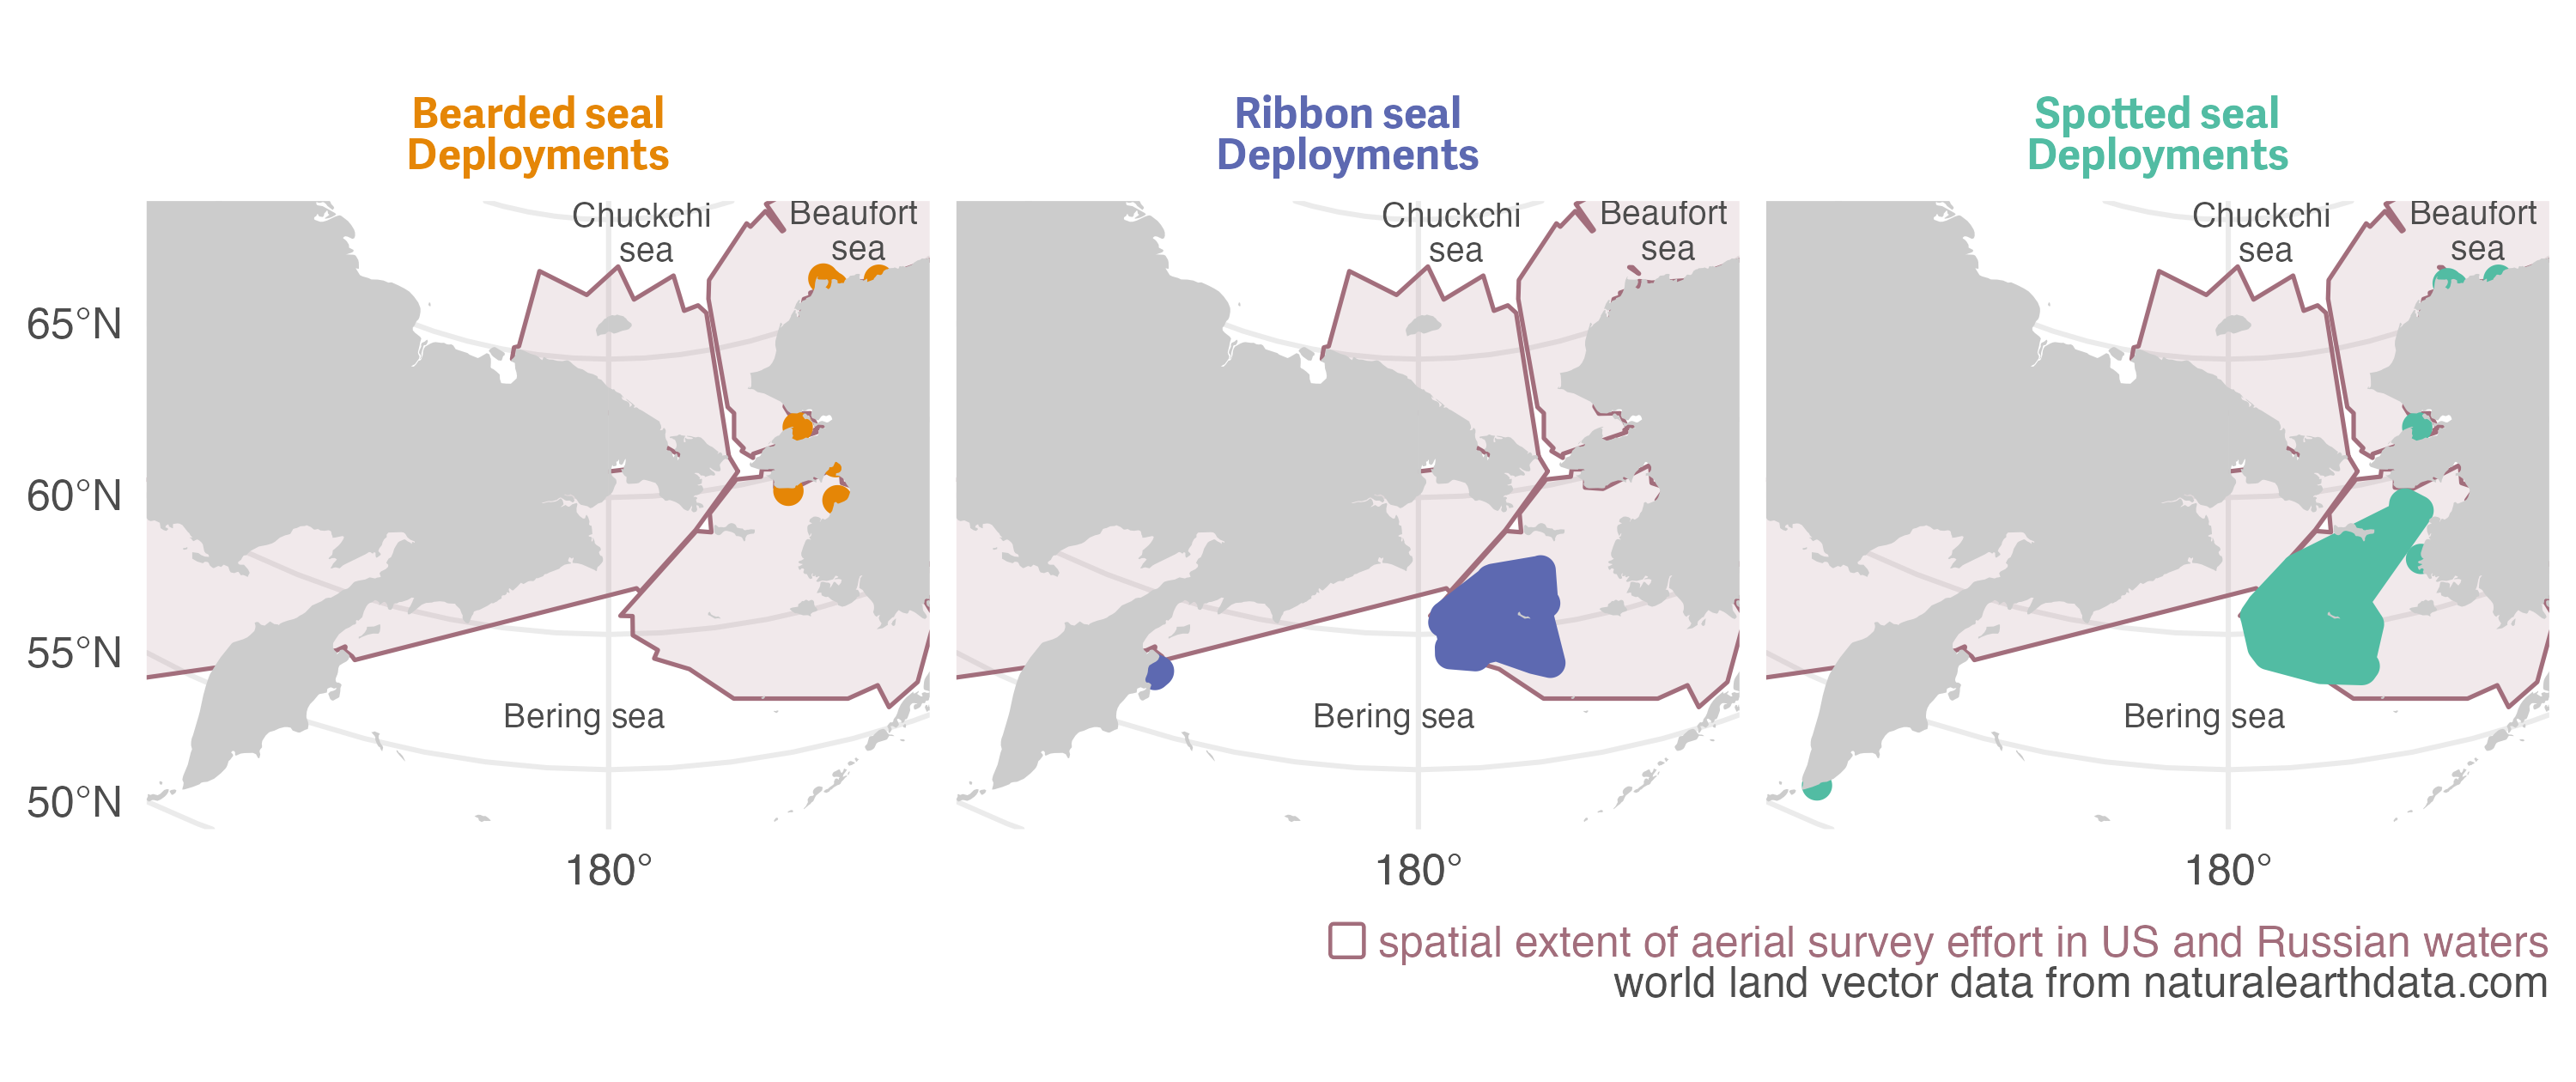
\includegraphics[width=1\linewidth]{../figures/Figure-001} \caption{\textbf{Initial bio-logger deployment areas for bearded, ribbon, and spotted seals in the study between 2005 and 2020 across multiple regions within the Bering, Chukchi, and western Beaufort seas.} \linebreak Solid regions shown for each species are minimum concave polygons buffered by 60 km for enhanced visibility. The larger, shaded region indicates the spatial extent of aerial survey effort to date in the Bering, Chukchi, and Beaufort seas. Deployments were initiated across a range of months but only haul-out data from 1 March to 15 July were included in the analysis. See Figure \ref{fig:dataMap} for the spatial distribution of observed data used in the study and Supplemental Materials \ref{tab:deploymentTable} for additional deployment details. World land vector data from \url{https://naturalearthdata.com}.}\label{fig:deployplot}
\end{figure}

We created a subset of haul-out behavior data from
250 bio-loggers deployed on
35 bearded,
110 ribbon, and
105 spotted seals
to include only records from 1 March to 15 July between
2005 and
2022. Bio-loggers were of the
`SPLASH' or `SPOT' family of tags developed by Wildlife Computers (Redmond,
Washington, USA). Deployments consisted of either a single `SPLASH' device, a
single `SPOT' device, or both types. Devices were either adhered to the hair on
the seal or attached through the rear flipper inter-digital webbing. The use of
bio-loggers adhered to the back or head provides some benefits over flipper
mounted devices (e.g.~increased satellite transmittal rates, locations at sea)
but these fall off during the following annual molt, which, depending on
deployment date, limits the duration of haul-out data they provide especially
during the focus months of our study. Additionally, bio-loggers attached to the
head or dorsal region are often dry while the seal is floating at the surface,
inducing a slight positive bias in the hourly percent-dry values reported by the
bio-logger. For this study, in cases where both bio-logger types were deployed,
we preferred hourly percent-dry observations from the flipper tag. All data were
transmitted by the deployed instruments via the Argos satellite network and
location data were either derived from Argos transmissions or transmitted
FastLoc GPS data.

Sex and age class (non-dependent \emph{young-of-the-year}, sexually immature
\emph{subadults}, and mature \emph{adults}) were estimated at the time of deployment by
various combinations of length, claw growth ridges (McLaren, 1958), and pelage
characteristics. Seals determined to be less than one year were classified as
young-of-the-year. For those bio-loggers deployed on young-of-the-year and
transmitting into the next year (6 ribbon seals; 3 spotted seals), the age class
was advanced to subadult on 1 March of the following year -- the assumed
anniversary of their birth. Subadults are those seals likely greater than one
year of age but less than four years. Adults are individuals that are likely
older than four years. Table \ref{tab:tblDeploy} provides a summary of these
deployments and data received from them.



\global\setlength{\Oldarrayrulewidth}{\arrayrulewidth}

\global\setlength{\Oldtabcolsep}{\tabcolsep}

\setlength{\tabcolsep}{2pt}

\renewcommand*{\arraystretch}{1.5}



\providecommand{\ascline}[3]{\noalign{\global\arrayrulewidth #1}\arrayrulecolor[HTML]{#2}\cline{#3}}

\begin{longtable}[c]{|p{0.90in}|p{0.40in}|p{1.35in}|p{1.35in}|p{1.35in}}

\caption{\textbf{Summary of bio-logger data by seal species and age classification from 1 March to 15 July 2005-2021.} \linebreak Seal hours represents the sum of hourly observations across all seals used in the analysis. Because young-of-the-year are advanced to subadult on 1 March of the following year, some individual seals are represented in both columns in this table}\label{tab:tblDeploy}\\

\ascline{1.5pt}{666666}{1-5}

\multicolumn{2}{>{\centering}m{\dimexpr 1.3in+2\tabcolsep}}{\textcolor[HTML]{000000}{\fontsize{9}{9}\selectfont{}}} & \multicolumn{3}{>{\centering}m{\dimexpr 4.05in+4\tabcolsep}}{\textcolor[HTML]{000000}{\fontsize{9}{9}\selectfont{Age\ Class}}} \\

\ascline{1.5pt}{666666}{1-5}



\multicolumn{1}{>{\raggedright}m{\dimexpr 0.9in+0\tabcolsep}}{\textcolor[HTML]{000000}{\fontsize{9}{9}\selectfont{Species}}} & \multicolumn{1}{>{\raggedright}m{\dimexpr 0.4in+0\tabcolsep}}{\textcolor[HTML]{000000}{\fontsize{9}{9}\selectfont{Sex}}} & \multicolumn{1}{>{\raggedright}m{\dimexpr 1.35in+0\tabcolsep}}{\textcolor[HTML]{000000}{\fontsize{9}{9}\selectfont{Adult}}} & \multicolumn{1}{>{\raggedright}m{\dimexpr 1.35in+0\tabcolsep}}{\textcolor[HTML]{000000}{\fontsize{9}{9}\selectfont{Subadult}}} & \multicolumn{1}{>{\raggedright}m{\dimexpr 1.35in+0\tabcolsep}}{\textcolor[HTML]{000000}{\fontsize{9}{9}\selectfont{Young-of-the-Year}}} \\

\ascline{1.5pt}{666666}{1-5}\endfirsthead \caption[]{\textbf{Summary of bio-logger data by seal species and age classification from 1 March to 15 July 2005-2021.} \linebreak Seal hours represents the sum of hourly observations across all seals used in the analysis. Because young-of-the-year are advanced to subadult on 1 March of the following year, some individual seals are represented in both columns in this table}\label{tab:tblDeploy}\\

\ascline{1.5pt}{666666}{1-5}

\multicolumn{2}{>{\centering}m{\dimexpr 1.3in+2\tabcolsep}}{\textcolor[HTML]{000000}{\fontsize{9}{9}\selectfont{}}} & \multicolumn{3}{>{\centering}m{\dimexpr 4.05in+4\tabcolsep}}{\textcolor[HTML]{000000}{\fontsize{9}{9}\selectfont{Age\ Class}}} \\

\ascline{1.5pt}{666666}{1-5}



\multicolumn{1}{>{\raggedright}m{\dimexpr 0.9in+0\tabcolsep}}{\textcolor[HTML]{000000}{\fontsize{9}{9}\selectfont{Species}}} & \multicolumn{1}{>{\raggedright}m{\dimexpr 0.4in+0\tabcolsep}}{\textcolor[HTML]{000000}{\fontsize{9}{9}\selectfont{Sex}}} & \multicolumn{1}{>{\raggedright}m{\dimexpr 1.35in+0\tabcolsep}}{\textcolor[HTML]{000000}{\fontsize{9}{9}\selectfont{Adult}}} & \multicolumn{1}{>{\raggedright}m{\dimexpr 1.35in+0\tabcolsep}}{\textcolor[HTML]{000000}{\fontsize{9}{9}\selectfont{Subadult}}} & \multicolumn{1}{>{\raggedright}m{\dimexpr 1.35in+0\tabcolsep}}{\textcolor[HTML]{000000}{\fontsize{9}{9}\selectfont{Young-of-the-Year}}} \\

\ascline{1.5pt}{666666}{1-5}\endhead



\multicolumn{1}{>{\raggedright}m{\dimexpr 0.9in+0\tabcolsep}}{\textcolor[HTML]{000000}{\fontsize{9}{9}\selectfont{Bearded\ seal}}} & \multicolumn{1}{>{\raggedright}m{\dimexpr 0.4in+0\tabcolsep}}{\textcolor[HTML]{000000}{\fontsize{9}{9}\selectfont{F}}} & \multicolumn{1}{>{\raggedright}m{\dimexpr 1.35in+0\tabcolsep}}{\textcolor[HTML]{000000}{\fontsize{9}{9}\selectfont{1\ (\ 1,776\ seal\ hours)}}} & \multicolumn{1}{>{\raggedright}m{\dimexpr 1.35in+0\tabcolsep}}{\textcolor[HTML]{000000}{\fontsize{9}{9}\selectfont{16\ (21,648\ seal\ hours)}}} & \multicolumn{1}{>{\raggedright}m{\dimexpr 1.35in+0\tabcolsep}}{\textcolor[HTML]{000000}{\fontsize{9}{9}\selectfont{}}} \\





\multicolumn{1}{>{\raggedright}m{\dimexpr 0.9in+0\tabcolsep}}{\textcolor[HTML]{000000}{\fontsize{9}{9}\selectfont{Bearded\ seal}}} & \multicolumn{1}{>{\raggedright}m{\dimexpr 0.4in+0\tabcolsep}}{\textcolor[HTML]{000000}{\fontsize{9}{9}\selectfont{M}}} & \multicolumn{1}{>{\raggedright}m{\dimexpr 1.35in+0\tabcolsep}}{\textcolor[HTML]{000000}{\fontsize{9}{9}\selectfont{2\ (\ 2,108\ seal\ hours)}}} & \multicolumn{1}{>{\raggedright}m{\dimexpr 1.35in+0\tabcolsep}}{\textcolor[HTML]{000000}{\fontsize{9}{9}\selectfont{16\ (17,232\ seal\ hours)}}} & \multicolumn{1}{>{\raggedright}m{\dimexpr 1.35in+0\tabcolsep}}{\textcolor[HTML]{000000}{\fontsize{9}{9}\selectfont{}}} \\





\multicolumn{1}{>{\raggedright}m{\dimexpr 0.9in+0\tabcolsep}}{\textcolor[HTML]{000000}{\fontsize{9}{9}\selectfont{Ribbon\ seal}}} & \multicolumn{1}{>{\raggedright}m{\dimexpr 0.4in+0\tabcolsep}}{\textcolor[HTML]{000000}{\fontsize{9}{9}\selectfont{F}}} & \multicolumn{1}{>{\raggedright}m{\dimexpr 1.35in+0\tabcolsep}}{\textcolor[HTML]{000000}{\fontsize{9}{9}\selectfont{33\ (35,128\ seal\ hours)}}} & \multicolumn{1}{>{\raggedright}m{\dimexpr 1.35in+0\tabcolsep}}{\textcolor[HTML]{000000}{\fontsize{9}{9}\selectfont{18\ (15,984\ seal\ hours)}}} & \multicolumn{1}{>{\raggedright}m{\dimexpr 1.35in+0\tabcolsep}}{\textcolor[HTML]{000000}{\fontsize{9}{9}\selectfont{13\ (\ 3,734\ seal\ hours)}}} \\





\multicolumn{1}{>{\raggedright}m{\dimexpr 0.9in+0\tabcolsep}}{\textcolor[HTML]{000000}{\fontsize{9}{9}\selectfont{Ribbon\ seal}}} & \multicolumn{1}{>{\raggedright}m{\dimexpr 0.4in+0\tabcolsep}}{\textcolor[HTML]{000000}{\fontsize{9}{9}\selectfont{M}}} & \multicolumn{1}{>{\raggedright}m{\dimexpr 1.35in+0\tabcolsep}}{\textcolor[HTML]{000000}{\fontsize{9}{9}\selectfont{24\ (27,465\ seal\ hours)}}} & \multicolumn{1}{>{\raggedright}m{\dimexpr 1.35in+0\tabcolsep}}{\textcolor[HTML]{000000}{\fontsize{9}{9}\selectfont{19\ (13,046\ seal\ hours)}}} & \multicolumn{1}{>{\raggedright}m{\dimexpr 1.35in+0\tabcolsep}}{\textcolor[HTML]{000000}{\fontsize{9}{9}\selectfont{9\ (\ 4,228\ seal\ hours)}}} \\





\multicolumn{1}{>{\raggedright}m{\dimexpr 0.9in+0\tabcolsep}}{\textcolor[HTML]{000000}{\fontsize{9}{9}\selectfont{Spotted\ seal}}} & \multicolumn{1}{>{\raggedright}m{\dimexpr 0.4in+0\tabcolsep}}{\textcolor[HTML]{000000}{\fontsize{9}{9}\selectfont{F}}} & \multicolumn{1}{>{\raggedright}m{\dimexpr 1.35in+0\tabcolsep}}{\textcolor[HTML]{000000}{\fontsize{9}{9}\selectfont{23\ (21,970\ seal\ hours)}}} & \multicolumn{1}{>{\raggedright}m{\dimexpr 1.35in+0\tabcolsep}}{\textcolor[HTML]{000000}{\fontsize{9}{9}\selectfont{21\ (19,559\ seal\ hours)}}} & \multicolumn{1}{>{\raggedright}m{\dimexpr 1.35in+0\tabcolsep}}{\textcolor[HTML]{000000}{\fontsize{9}{9}\selectfont{11\ (13,417\ seal\ hours)}}} \\





\multicolumn{1}{>{\raggedright}m{\dimexpr 0.9in+0\tabcolsep}}{\textcolor[HTML]{000000}{\fontsize{9}{9}\selectfont{Spotted\ seal}}} & \multicolumn{1}{>{\raggedright}m{\dimexpr 0.4in+0\tabcolsep}}{\textcolor[HTML]{000000}{\fontsize{9}{9}\selectfont{M}}} & \multicolumn{1}{>{\raggedright}m{\dimexpr 1.35in+0\tabcolsep}}{\textcolor[HTML]{000000}{\fontsize{9}{9}\selectfont{20\ (31,793\ seal\ hours)}}} & \multicolumn{1}{>{\raggedright}m{\dimexpr 1.35in+0\tabcolsep}}{\textcolor[HTML]{000000}{\fontsize{9}{9}\selectfont{21\ (17,210\ seal\ hours)}}} & \multicolumn{1}{>{\raggedright}m{\dimexpr 1.35in+0\tabcolsep}}{\textcolor[HTML]{000000}{\fontsize{9}{9}\selectfont{12\ (11,285\ seal\ hours)}}} \\

\ascline{1.5pt}{666666}{1-5}



\end{longtable}



\arrayrulecolor[HTML]{000000}

\global\setlength{\arrayrulewidth}{\Oldarrayrulewidth}

\global\setlength{\tabcolsep}{\Oldtabcolsep}

\renewcommand*{\arraystretch}{1}

Haul-out behavior data were recorded in a manner standard across Wildlife
Computers bio-loggers and transmitted via the Argos satellite network as hourly
percent-dry timelines. For each hour of a day, the wet/dry sensor was polled by
the tag firmware every few seconds and the percent of the hour in the dry state
was calculated (Figure \ref{fig:examplePlot}). On board the bio-logger, hourly
percent-dry calculations were rounded to the nearest 10\% inclusive of 0\% and
100\% along with additional values at 3\% and 98\%. This compression resulted in
additional data transmission as each message consisted of two complete 24-hour
records. Memory capacity allowed caching of percent-dry records for several
weeks or months and each message was transmitted several times to ensure
reception at the satellite. Bio-loggers were deployed and programmed in a manner
to maximize data transmission during the spring pupping and molting period,
though hourly percent-dry data were not always successfully transmitted. This is
due to a variety of factors including satellite coverage, tag availability
(e.g., tags mounted to the rear flipper often do not transmit while at sea), tag
performance, duty cycling, and atmospheric interference. Fortunately, missing
records do not substantially bias inference about haul-out probabilities
(Conn et al., 2012).

Tags that fell off due to molt, attachment failure, or seal mortality and remained
on ice or land may have continued to send data to satellites; i.e., a detached
bio-logger that is dry (either on ice or land) will record and transmit data
suggesting the seal is hauled out. Therefore, end times of each deployment were
identified by examining bio-logger locations, percent-dry records, and dive
behavior (if available) to determine when bio-loggers ceased providing data
consistent with seal behavior. For example, a data record that ended with several
consecutive days (\textasciitilde10+ days) of 100\% dry observations and with locations
indicating the tag was on land were truncated to the final
stretch of 100\% dry observations. The vast majority of deployments ended with the
device detaching in the water and the deployment end date was obvious. There is
no perfect algorithm for identifying deployment end dates and each deployment in
question was considered separately. While not perfect, we are confident our
reliance on expert opinion and examination of multiple data streams provided the
best option. Data outside of the deployment start and end times were discarded
prior to analysis.










\begin{figure}
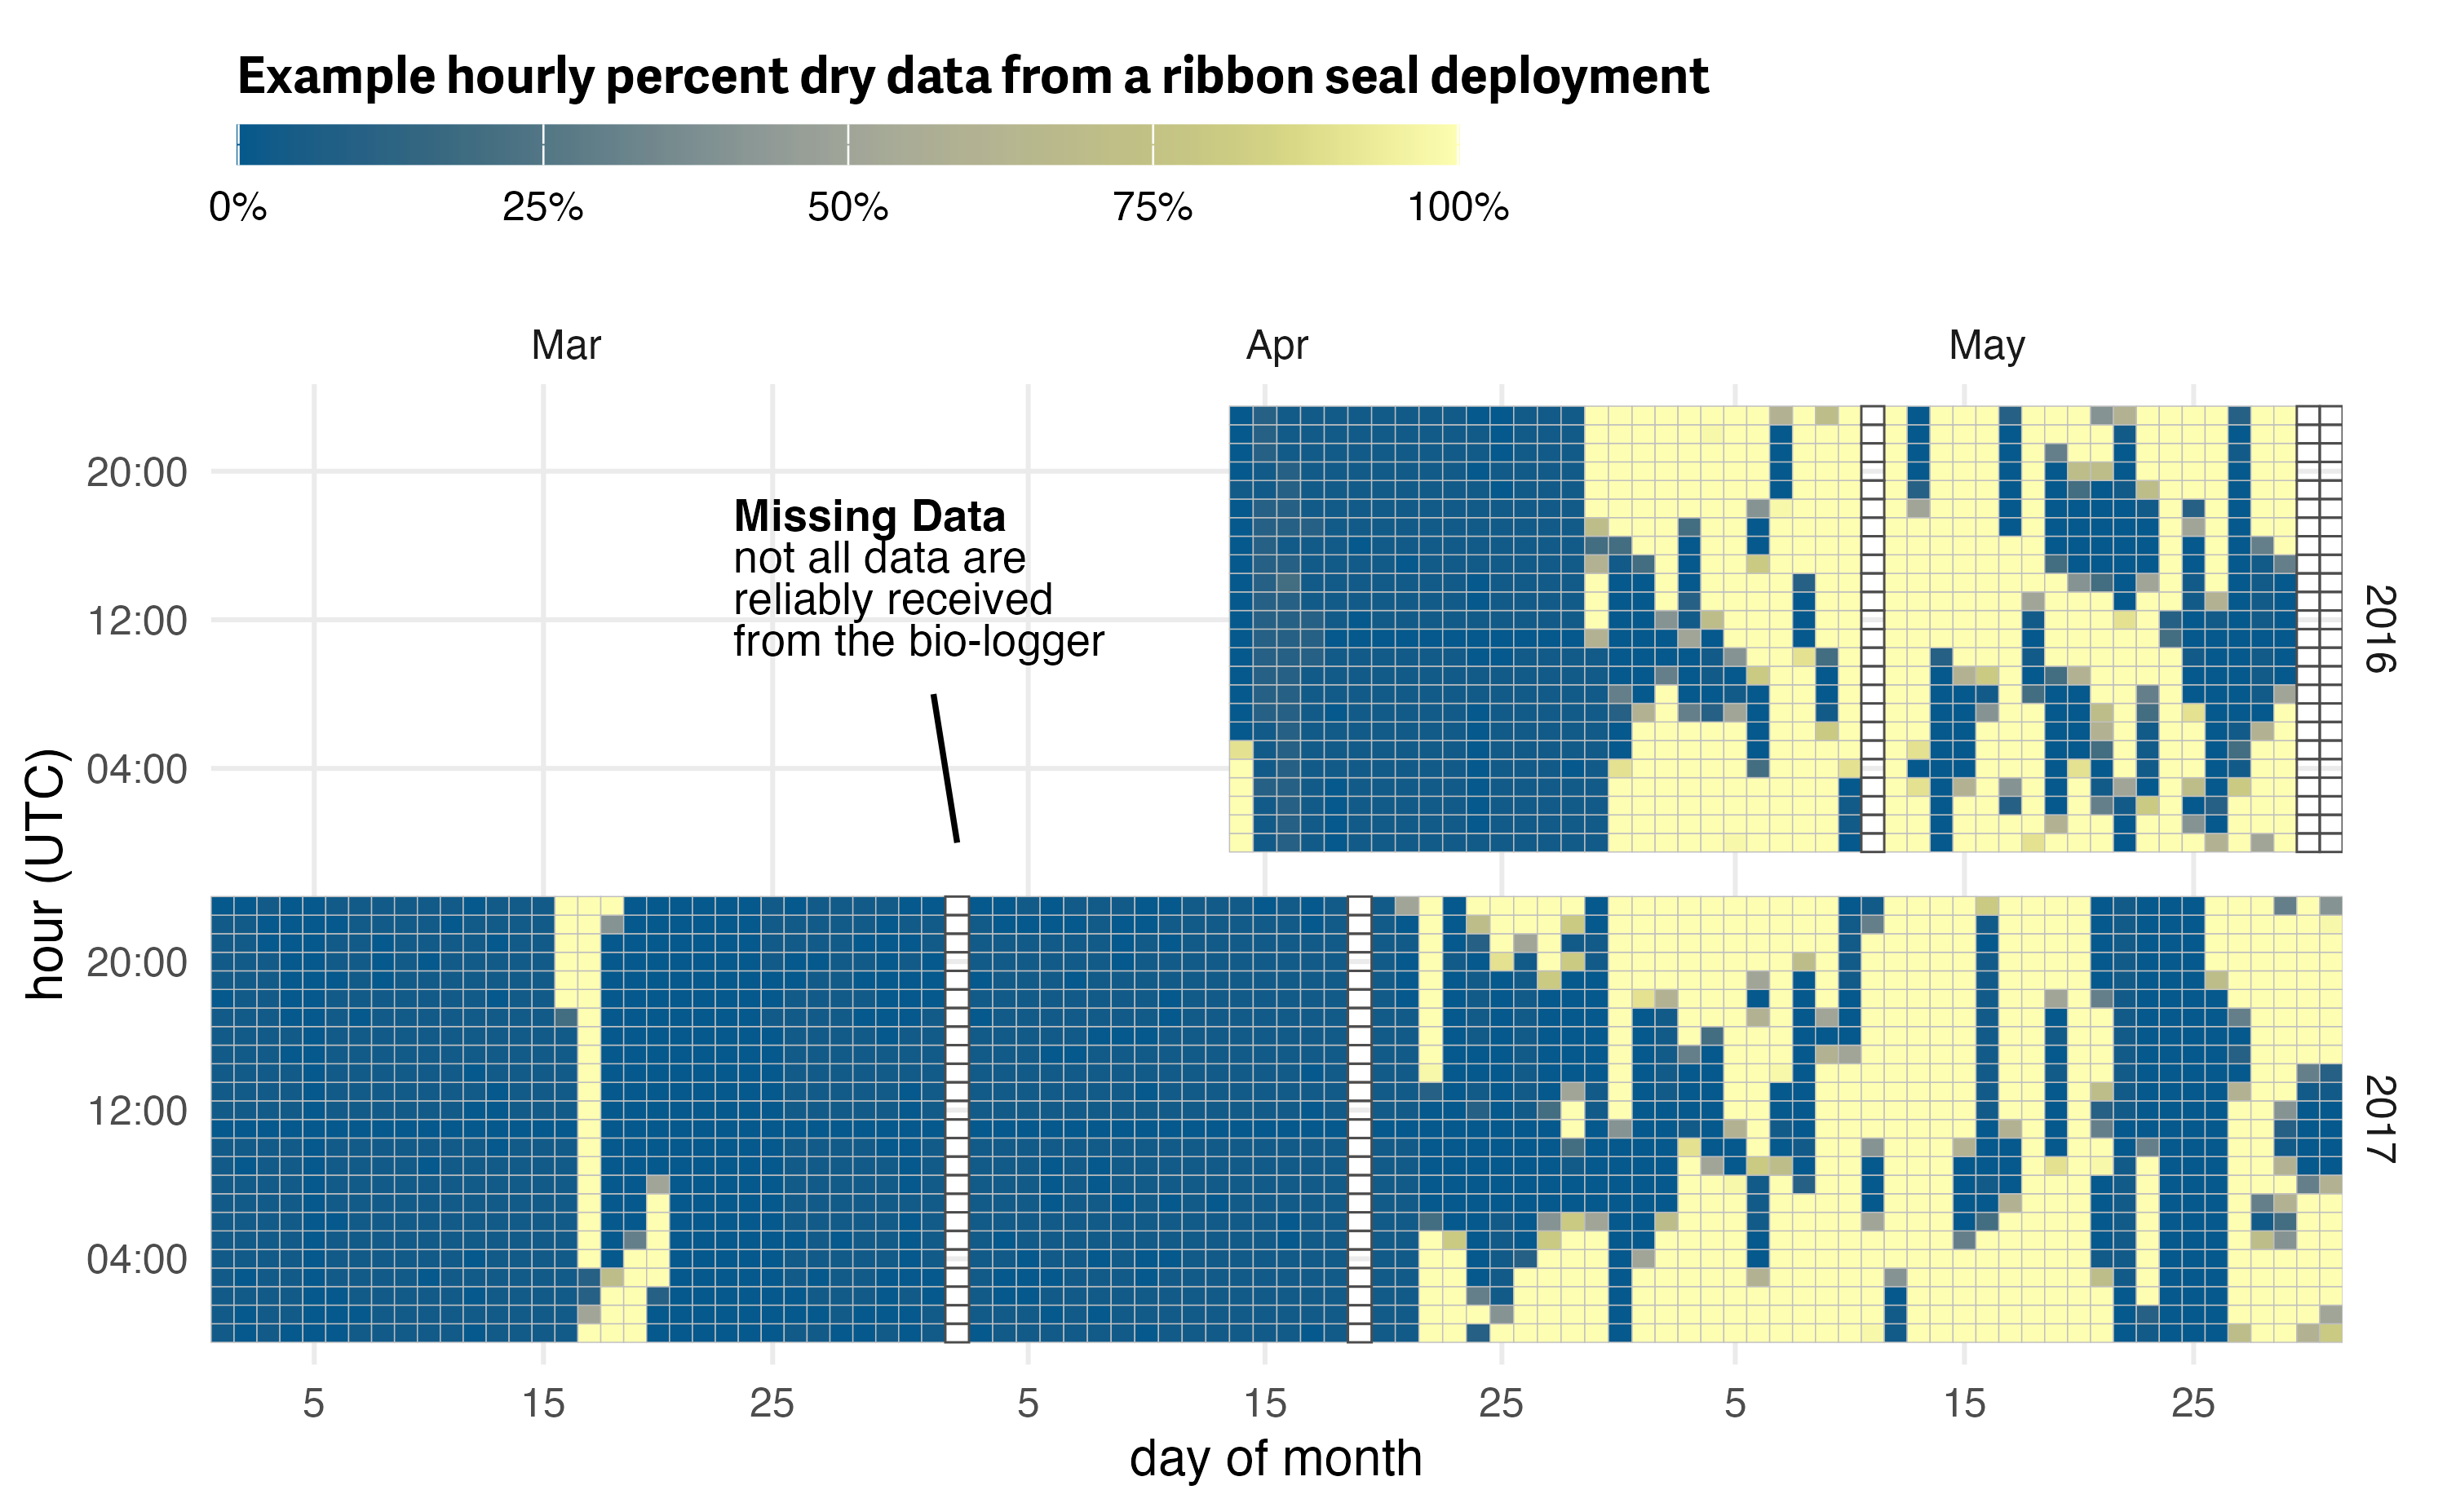
\includegraphics[width=1\linewidth]{../figures/Figure-002} \caption{\textbf{Example percent-dry actogram from bio-logger data}
\linebreak Haul-out behavior observations recorded by a bio-logger deployed on a
ribbon seal over two years during the months of March, April, and May. This
actogram plot represents the transmitted hourly percent-dry values. Not all data
during a deployment are reliably transmitted from the bio-logger and because data
are transmitted in 24-hour chunks occasional missing days are present in the
record. Here, missing data that were not successfully received from the device
are represented as empty rectangles.}\label{fig:examplePlot}
\end{figure}

Of key interest in this study was the relationship between haul-out behavior and
weather covariates that vary with time and seal location. The use of modern
bio-loggers that record and transmit behavioral data while simultaneously
providing location estimates was key to this objective. We explored the use
of a continuous-time correlated random walk (Johnson et al., 2008) movement model
to predict locations at specific times. However, the sparse nature of data from
some bio-loggers, especially those mounted to the rear flipper, resulted in poor
modeling performance or convergence issues. For this study, we calculated a
weighted average daily location where the inverse of the estimated Argos or
FastLoc GPS location error was used for the weight. Each Argos location estimate
was assigned an error radius based on either the categorical location quality (
\emph{3} = 250 m, \emph{2} = 500 m, \emph{1} = 1500 m, \emph{0} = 2500 m (Lopez et al., 2013); we chose 2500 m for
location classes \emph{A} and \emph{B}) or, when available, the estimated error radius
from the Argos Kalman filter algorithm. Location estimates from FastLoc GPS were
all assigned an error radius of 50 m. On days when haul-out observations were
present but location data were missing we used the seal's last calculated weighted
average daily location; days when the location intersected with land
were removed from the seal's record. We recognize that bearded and spotted
seals haul out on land. However, assessing the relationship between haul-out
behavior and weather covariates and seals' availability for aerial surveys on
land was outside the scope of this study. Additionally, any daily locations on
land were likely more reflective of coordinate averaging and measurement error,
rather than actual use of coastal features.

\subsection*{Explanatory variables}\label{explanatory-variables}
\addcontentsline{toc}{subsection}{Explanatory variables}

In addition to sex and age class, we analyzed variables that might help explain
variation in haul-out probabilities. These included day-of-year (for seasonal
effects) and local solar hour (for diurnal effects). We calculated local solar
hour using the \{solaR\} package (Perpiñán, 2012) within the R statistical
environment (R Core Team, 2021) based on the weighted daily average locations. We
also linked the weighted average daily locations to weather values from the
North American Regional Reanalysis (NARR) model produced by the National Centers
for Environmental Prediction (Mesinger et al., 2006). The NARR model assimilates
observational data to produce a long-term picture of weather over North America
and portions of the surrounding seas. Weather variables are made available
across the region 8 times daily. For this study, NARR weather values were limited
to the extent of our study area over the Bering, Chukchi, and Beaufort seas at 3-hr
intervals based on the original grid resolution of 32 km (1024 km\textsuperscript{2}). The
following weather variables are known to affect haul-out behavior in
other Arctic pinnipeds (Reder et al., 2003; Udevitz et al., 2009; Perry, Stenson \& Buren, 2017) and were
interpolated and assigned to daily seal locations using a bilinear method: 1)
air temperature at 2 m above the Earth's surface, 2) wind consisting of
northerly and easterly vector components converted to wind speed using the
Euclidean norm, 3) barometric pressure at sea level, and 4) precipitation
(Table \ref{tab:tblCovariates}).

For all seal species, we considered the following variables when modeling the
hourly haul-out behavior: day-of-year, solar hour, temperature, wind speed,
barometric pressure, precipitation, and wind chill (represented by a
\emph{wind:temperature} interaction (Udevitz et al., 2009)). Ribbon and spotted seal models
included age-sex class and interactions between day-of-year and age-sex class,
but we omitted these from bearded seal models due to poor representation of
age-sex classes (Table \ref{tab:tblDeploy}). Bearded seal models included a
latitudinal effect (and an interaction with day-of-year), because bearded seals
occupy a substantial range during the spring and we were interested in possible
differences in the timing of haul-out behavior along a latitudinal gradient. We
omitted the latitudinal effect from ribbon and spotted seal models because,
during the spring, these species are most prevalent near the southern ice edge
in the Bering Sea (Conn et al., 2014).





\global\setlength{\Oldarrayrulewidth}{\arrayrulewidth}

\global\setlength{\Oldtabcolsep}{\tabcolsep}

\setlength{\tabcolsep}{2pt}

\renewcommand*{\arraystretch}{1.5}



\providecommand{\ascline}[3]{\noalign{\global\arrayrulewidth #1}\arrayrulecolor[HTML]{#2}\cline{#3}}

\begin{longtable}[c]{|p{1.00in}|p{1.00in}|p{2.50in}}

\caption{\textbf{Explanatory covariates used in analyses of binary haul-out records for bearded, spotted, and ribbon seals.} \linebreak Note that we also considered select interactions (see article text) between these primary covariates. For instance, wind chill was represented by the interaction temperature:wind.}\label{tab:tblCovariates}\\

\ascline{1.5pt}{666666}{1-3}

\multicolumn{1}{>{\raggedright}m{\dimexpr 1in+0\tabcolsep}}{\textcolor[HTML]{000000}{\fontsize{9}{9}\selectfont{Covariate}}} & \multicolumn{1}{>{\raggedright}m{\dimexpr 1in+0\tabcolsep}}{\textcolor[HTML]{000000}{\fontsize{9}{9}\selectfont{Type}}} & \multicolumn{1}{>{\raggedright}m{\dimexpr 2.5in+0\tabcolsep}}{\textcolor[HTML]{000000}{\fontsize{9}{9}\selectfont{Description}}} \\

\ascline{1.5pt}{666666}{1-3}\endfirsthead \caption[]{\textbf{Explanatory covariates used in analyses of binary haul-out records for bearded, spotted, and ribbon seals.} \linebreak Note that we also considered select interactions (see article text) between these primary covariates. For instance, wind chill was represented by the interaction temperature:wind.}\label{tab:tblCovariates}\\

\ascline{1.5pt}{666666}{1-3}

\multicolumn{1}{>{\raggedright}m{\dimexpr 1in+0\tabcolsep}}{\textcolor[HTML]{000000}{\fontsize{9}{9}\selectfont{Covariate}}} & \multicolumn{1}{>{\raggedright}m{\dimexpr 1in+0\tabcolsep}}{\textcolor[HTML]{000000}{\fontsize{9}{9}\selectfont{Type}}} & \multicolumn{1}{>{\raggedright}m{\dimexpr 2.5in+0\tabcolsep}}{\textcolor[HTML]{000000}{\fontsize{9}{9}\selectfont{Description}}} \\

\ascline{1.5pt}{666666}{1-3}\endhead



\multicolumn{1}{>{\raggedright}m{\dimexpr 1in+0\tabcolsep}}{\textcolor[HTML]{000000}{\fontsize{9}{9}\selectfont{Age-sex\ class}}} & \multicolumn{1}{>{\raggedright}m{\dimexpr 1in+0\tabcolsep}}{\textcolor[HTML]{000000}{\fontsize{9}{9}\selectfont{Categorical}}} & \multicolumn{1}{>{\raggedright}m{\dimexpr 2.5in+0\tabcolsep}}{\textcolor[HTML]{000000}{\fontsize{9}{9}\selectfont{young-of-the-year,\ subadult,\ adult\ male\ and\ adult\ female}}} \\





\multicolumn{1}{>{\raggedright}m{\dimexpr 1in+0\tabcolsep}}{\textcolor[HTML]{000000}{\fontsize{9}{9}\selectfont{Hour}}} & \multicolumn{1}{>{\raggedright}m{\dimexpr 1in+0\tabcolsep}}{\textcolor[HTML]{000000}{\fontsize{9}{9}\selectfont{Continuous;\ Fourier\ basis}}} & \multicolumn{1}{>{\raggedright}m{\dimexpr 2.5in+0\tabcolsep}}{\textcolor[HTML]{000000}{\fontsize{9}{9}\selectfont{local\ solar\ hour\ using\ 6\ variables\ of\ a\ Fourier-series\ basis}}} \\





\multicolumn{1}{>{\raggedright}m{\dimexpr 1in+0\tabcolsep}}{\textcolor[HTML]{000000}{\fontsize{9}{9}\selectfont{Day}}} & \multicolumn{1}{>{\raggedright}m{\dimexpr 1in+0\tabcolsep}}{\textcolor[HTML]{000000}{\fontsize{9}{9}\selectfont{Continuous}}} & \multicolumn{1}{>{\raggedright}m{\dimexpr 2.5in+0\tabcolsep}}{\textcolor[HTML]{000000}{\fontsize{9}{9}\selectfont{linear,\ quadratic,\ and\ cubic\ effects\ of\ day-of-year}}} \\





\multicolumn{1}{>{\raggedright}m{\dimexpr 1in+0\tabcolsep}}{\textcolor[HTML]{000000}{\fontsize{9}{9}\selectfont{Precip}}} & \multicolumn{1}{>{\raggedright}m{\dimexpr 1in+0\tabcolsep}}{\textcolor[HTML]{000000}{\fontsize{9}{9}\selectfont{Continuous}}} & \multicolumn{1}{>{\raggedright}m{\dimexpr 2.5in+0\tabcolsep}}{\textcolor[HTML]{000000}{\fontsize{9}{9}\selectfont{convective\ precipitation\ kg/m\textsuperscript{2}\ (NARR)}}} \\





\multicolumn{1}{>{\raggedright}m{\dimexpr 1in+0\tabcolsep}}{\textcolor[HTML]{000000}{\fontsize{9}{9}\selectfont{Pressure}}} & \multicolumn{1}{>{\raggedright}m{\dimexpr 1in+0\tabcolsep}}{\textcolor[HTML]{000000}{\fontsize{9}{9}\selectfont{Continuous}}} & \multicolumn{1}{>{\raggedright}m{\dimexpr 2.5in+0\tabcolsep}}{\textcolor[HTML]{000000}{\fontsize{9}{9}\selectfont{atmospheric\ pressure\ at\ sea\ level\ (kPa)\ (NARR)}}} \\





\multicolumn{1}{>{\raggedright}m{\dimexpr 1in+0\tabcolsep}}{\textcolor[HTML]{000000}{\fontsize{9}{9}\selectfont{Temp}}} & \multicolumn{1}{>{\raggedright}m{\dimexpr 1in+0\tabcolsep}}{\textcolor[HTML]{000000}{\fontsize{9}{9}\selectfont{Continuous}}} & \multicolumn{1}{>{\raggedright}m{\dimexpr 2.5in+0\tabcolsep}}{\textcolor[HTML]{000000}{\fontsize{9}{9}\selectfont{air\ temperature\ (C)\ at\ 2m\ above\ the\ earth’s\ surface\ (NARR)}}} \\





\multicolumn{1}{>{\raggedright}m{\dimexpr 1in+0\tabcolsep}}{\textcolor[HTML]{000000}{\fontsize{9}{9}\selectfont{Wind}}} & \multicolumn{1}{>{\raggedright}m{\dimexpr 1in+0\tabcolsep}}{\textcolor[HTML]{000000}{\fontsize{9}{9}\selectfont{Continuous}}} & \multicolumn{1}{>{\raggedright}m{\dimexpr 2.5in+0\tabcolsep}}{\textcolor[HTML]{000000}{\fontsize{9}{9}\selectfont{northerly\ and\ easterly\ vector\ components\ for\ wind\ (NARR)\ converted\ into\ a\ single\ wind\ speed\ via\ the\ Euclidean\ norm}}} \\





\multicolumn{1}{>{\raggedright}m{\dimexpr 1in+0\tabcolsep}}{\textcolor[HTML]{000000}{\fontsize{9}{9}\selectfont{Northing}}} & \multicolumn{1}{>{\raggedright}m{\dimexpr 1in+0\tabcolsep}}{\textcolor[HTML]{000000}{\fontsize{9}{9}\selectfont{Continuous}}} & \multicolumn{1}{>{\raggedright}m{\dimexpr 2.5in+0\tabcolsep}}{\textcolor[HTML]{000000}{\fontsize{9}{9}\selectfont{latitude\ divided\ by\ the\ mean\ latitude\ across\ all\ locations\ (for\ bearded\ seals\ only)}}} \\

\ascline{1pt}{666666}{1-3}



\multicolumn{1}{>{\raggedright}m{\dimexpr 1in+0\tabcolsep}}{\textcolor[HTML]{000000}{\fontsize{9}{9}\selectfont{Year}}} & \multicolumn{1}{>{\raggedright}m{\dimexpr 1in+0\tabcolsep}}{\textcolor[HTML]{000000}{\fontsize{9}{9}\selectfont{Continuous}}} & \multicolumn{1}{>{\raggedright}m{\dimexpr 2.5in+0\tabcolsep}}{\textcolor[HTML]{000000}{\fontsize{9}{9}\selectfont{For\ the\ set\ of\ models\ examining\ inter-annual\ variation\ in\ sea-ice\ use,\ we\ fitted\ models\ with\ the\ addition\ of\ year\ by\ day-of-year\ interactions.}}} \\

\ascline{1.5pt}{666666}{1-3}



\end{longtable}



\arrayrulecolor[HTML]{000000}

\global\setlength{\arrayrulewidth}{\Oldarrayrulewidth}

\global\setlength{\tabcolsep}{\Oldtabcolsep}

\renewcommand*{\arraystretch}{1}

\subsection*{Haul-out modeling}\label{haul-out-modeling}
\addcontentsline{toc}{subsection}{Haul-out modeling}

Haul-out records for seals are often characterized by sequential hours spent
hauled out on ice alternating with long periods in the water (Figure
\ref{fig:examplePlot}). Commonly used statistical models for binary data (e.g.
logistic regression) assume independence among responses, an assumption that is
clearly violated if hourly responses are modeled. Any analysis that ignores
temporal autocorrelation in responses will thus have overstated precision
(Betts et al., 2006).

To properly account for temporal dependence and to take advantage of
computational efficiency, we used generalized linear mixed pseudo-models
(GLMPMs; Ver Hoef, London \& Boveng (2010)) to model variation in
haul-out behavior as a function of (1) covariate predictors, (2) temporally
autocorrelated random effects, and (3) individual random effects representing
heterogeneity in individual behavior. We used the glmmLDTS package
(Ver Hoef, London \& Boveng, 2010) to implement GLMPMs. We explored two different model
formulations for our data and we fit separate models to bearded, ribbon, and
spotted seal data sets as we expected differing behavior by species. Separate
models for each species were also needed because a single, very large data set
proved computationally intractable. In our first model formulation and for each
species, we fitted a year-independent model that predicted average haul-out
behavior as a function of demographic, weather, seasonal, and diurnal effects.
Second, for ribbon and spotted seals (which had considerably more data than
bearded seals), we fitted models that included all the effects from the first
model, but also permitted annual variation in haul-out timing. This second set
of models was used to examine whether haul-out patterns varied by year and to
determine the annual timing of apparent peaks in haul-out behavior. For both
models, we assumed an hourly Bernoulli response (a binary 0-1 response dependent
upon whether the tag was greater than 50\% dry for a given hour) where the linear
predictor was modeled on the logit scale. This is
consistent with previous approaches (London et al., 2012; Ver Hoef et al., 2014) and only
7.005\% of our
observations fell between 10\% and 90\% hourly percent-dry.

We followed Ver Hoef et al. (2014) in using linear, quadratic, and cubic
effects of day-of-year to represent temporal changes
in behavior during the season. However, unlike previous models for harbor seals
(London et al., 2012) and ice-associated seals (Ver Hoef et al., 2014), which treated
hour-of-day as a 24-level categorical variable to capture diurnal cycles, we
adopted a continuous formulation based on Fourier series that provides a
flexible model while preserving the inherent circularity needed for time-of-day
effects (i.e., hour 0 should be equal to hour 24). It also represents
hour-of-day with 6 parameters, which is a considerable reduction when compared
to a 24-parameter variable. According to this approach, we used the following
specification for hour-of-day effects:

\[
H_t=\alpha_1 \cos(\frac{\pi t}{4}) + \alpha_2 \sin(\frac{\pi t}{4}) + \alpha_3 \cos(\frac{\pi t}{6}) + \alpha_4 \sin(\frac{\pi t}{6}) + \alpha_5 \cos(\frac{\pi t}{12}) + \alpha_6 \sin(\frac{\pi t}{12})
\]
where \(H_t\) gives the effect for solar hour \(t\) and \(\alpha_{i}\) are
estimated parameters (regression coefficients).

For the second set of models examining inter-annual variation in sea-ice use, we
fitted models with year by day-of-year interactions. However, in this case we
only included \emph{year:day} and \emph{year:day\textsuperscript{2}}, omitting the main effects of year as
well as \emph{year:day\textsuperscript{3}} interactions because models with the latter effects were
numerically unstable. However, the modeled interactions were sufficient to allow
shifts in haul-out distribution, as one can show mathematically that a simple
horizontal shift in timing of haul-out distributions does not affect the main
effects or cubic terms in a polynomial regression model. Bearded seals were
not included in this examination of inter-annual variation because of limited
data across many years in the study.

A typical model fitting exercise would also include a model selection process.
However, AIC (and similar criteria) is not suitable when using
pseudo-likelihoods, because pseudo-data generated in the model fitting process
(Ver Hoef, London \& Boveng, 2010) differ between models (Ten Eyck \& Cavanaugh, 2018). After fitting GLMPM
models, we instead used `type III' \(F\)-tests to calculate \(p\)-values
(Ver Hoef, London \& Boveng, 2010) to evaluate model performance and important terms. We also
produced predictions of haul-out behavior as a function of three influential
predictors (e.g.~solar hour, day-of-year, age-sex). Weather covariates for these
predictions were based on daily or hourly smoothed weather covariate values
across the study region. Such predictions were then used to develop haul-out
probability surfaces, explore conditional effects of weather covariates, and
determine annual peaks in haul-out activity. The timing of peak haul-out
behavior was further used to regress against the annual maximum sea-ice extent
in the study region. Predictions before 15 March and after 30 June were not
included in visualizations or other evaluations to avoid spurious model
predictions at the edge of the data range.

Visualizing the marginal or conditional effect of an individual weather
covariate (where all other weather covariates are being held at mean values) on
haul-out probability was difficult in this analysis because of the collinearity
between covariates as well as the spatial and temporal variation across such a
large region. The relationship of each weather covariate with haul-out
probability, averaged over the other weather conditions, was more variable than
model coefficients would imply. That said, important insights can be gained from
plots of marginal effects. To create these plots, we predicted haul-out
probability across the full range of each weather covariate while fixing hour
of the day at local solar noon and day-of-year at 15 May. For the other weather
covariate values, we chose not to use a fixed mean value because we expect weather
to vary within day over the season (e.g.~the temperature at solar noon will
gradually increase from March through June). To account for this, we fit a simple generalized
additive model for each weather covariate with smooth terms for day-of-year and
solar hour. We used predicted values from the generalized additive model in lieu
of holding other weather covariates at a fixed mean value which would not capture
seasonal change. The visualizations
also include vertical lines representing 95\% confidence intervals around the
predicted haul-out probability to better communicate the variation in model
uncertainty.

We also assessed whether the annual variation in maximum spring sea-ice extent in the
Bering Sea influenced the seasonal peak of seal haul-out probability. In
particular, we used sea-ice concentration data from the Nimbus-7 SMMR and DMSP
SSM/I-SSMIS Passive Microwave Dataset, Version 1 (Cavalieri et al., 1996) to calculate
maximum sea-ice extent. All sea-ice concentration grid cells (25 km\textsuperscript{2}) in the
study area with greater than 15\% concentration were counted daily to get the total sea
ice extent for each day between 15 February and 15 July across all years.
Maximum spring sea-ice extent was simply the largest daily count of grid cells
with greater than 15\% concentration for each year. A separate regression model,
built on the results of the haul-out model, was used to evaluate the relationship
between the annual computed peak haul-out day (as the response) with the
maximum sea-ice extent (as the predictor).

\section*{Results}\label{results}
\addcontentsline{toc}{section}{Results}

Figure \ref{fig:dataMap} shows the spatial distribution of weighted locations
with available haul-out behavior data used for analysis of each species across
the study area. Figure \ref{fig:dataCal} shows the temporal distribution of all
haul-out data across the study season for each species. Observations of ribbon
and spotted seals were concentrated in the months of May and June due to the
timing of deployment (April and May) and the timing of molt (May and June).
During molt, seals (and their attached bio-loggers) spend more time out of the
water and more data are transmitted. Molt timing also impacts when many
deployments end as any bio-loggers adhered to the hair will fall off. Relative
to the other species in the study, there were fewer deployments of bio-loggers
on bearded seals. This resulted in fewer data observations overall and
noticeably lower in numbers May and June. The majority of deployments on bearded
seals occurred in August and September and, by May, bio-loggers had either
fallen off or their batteries were depleted. Therefore, observations for bearded
seals were concentrated in March (Figure \ref{fig:dataCal}).



\begin{figure}
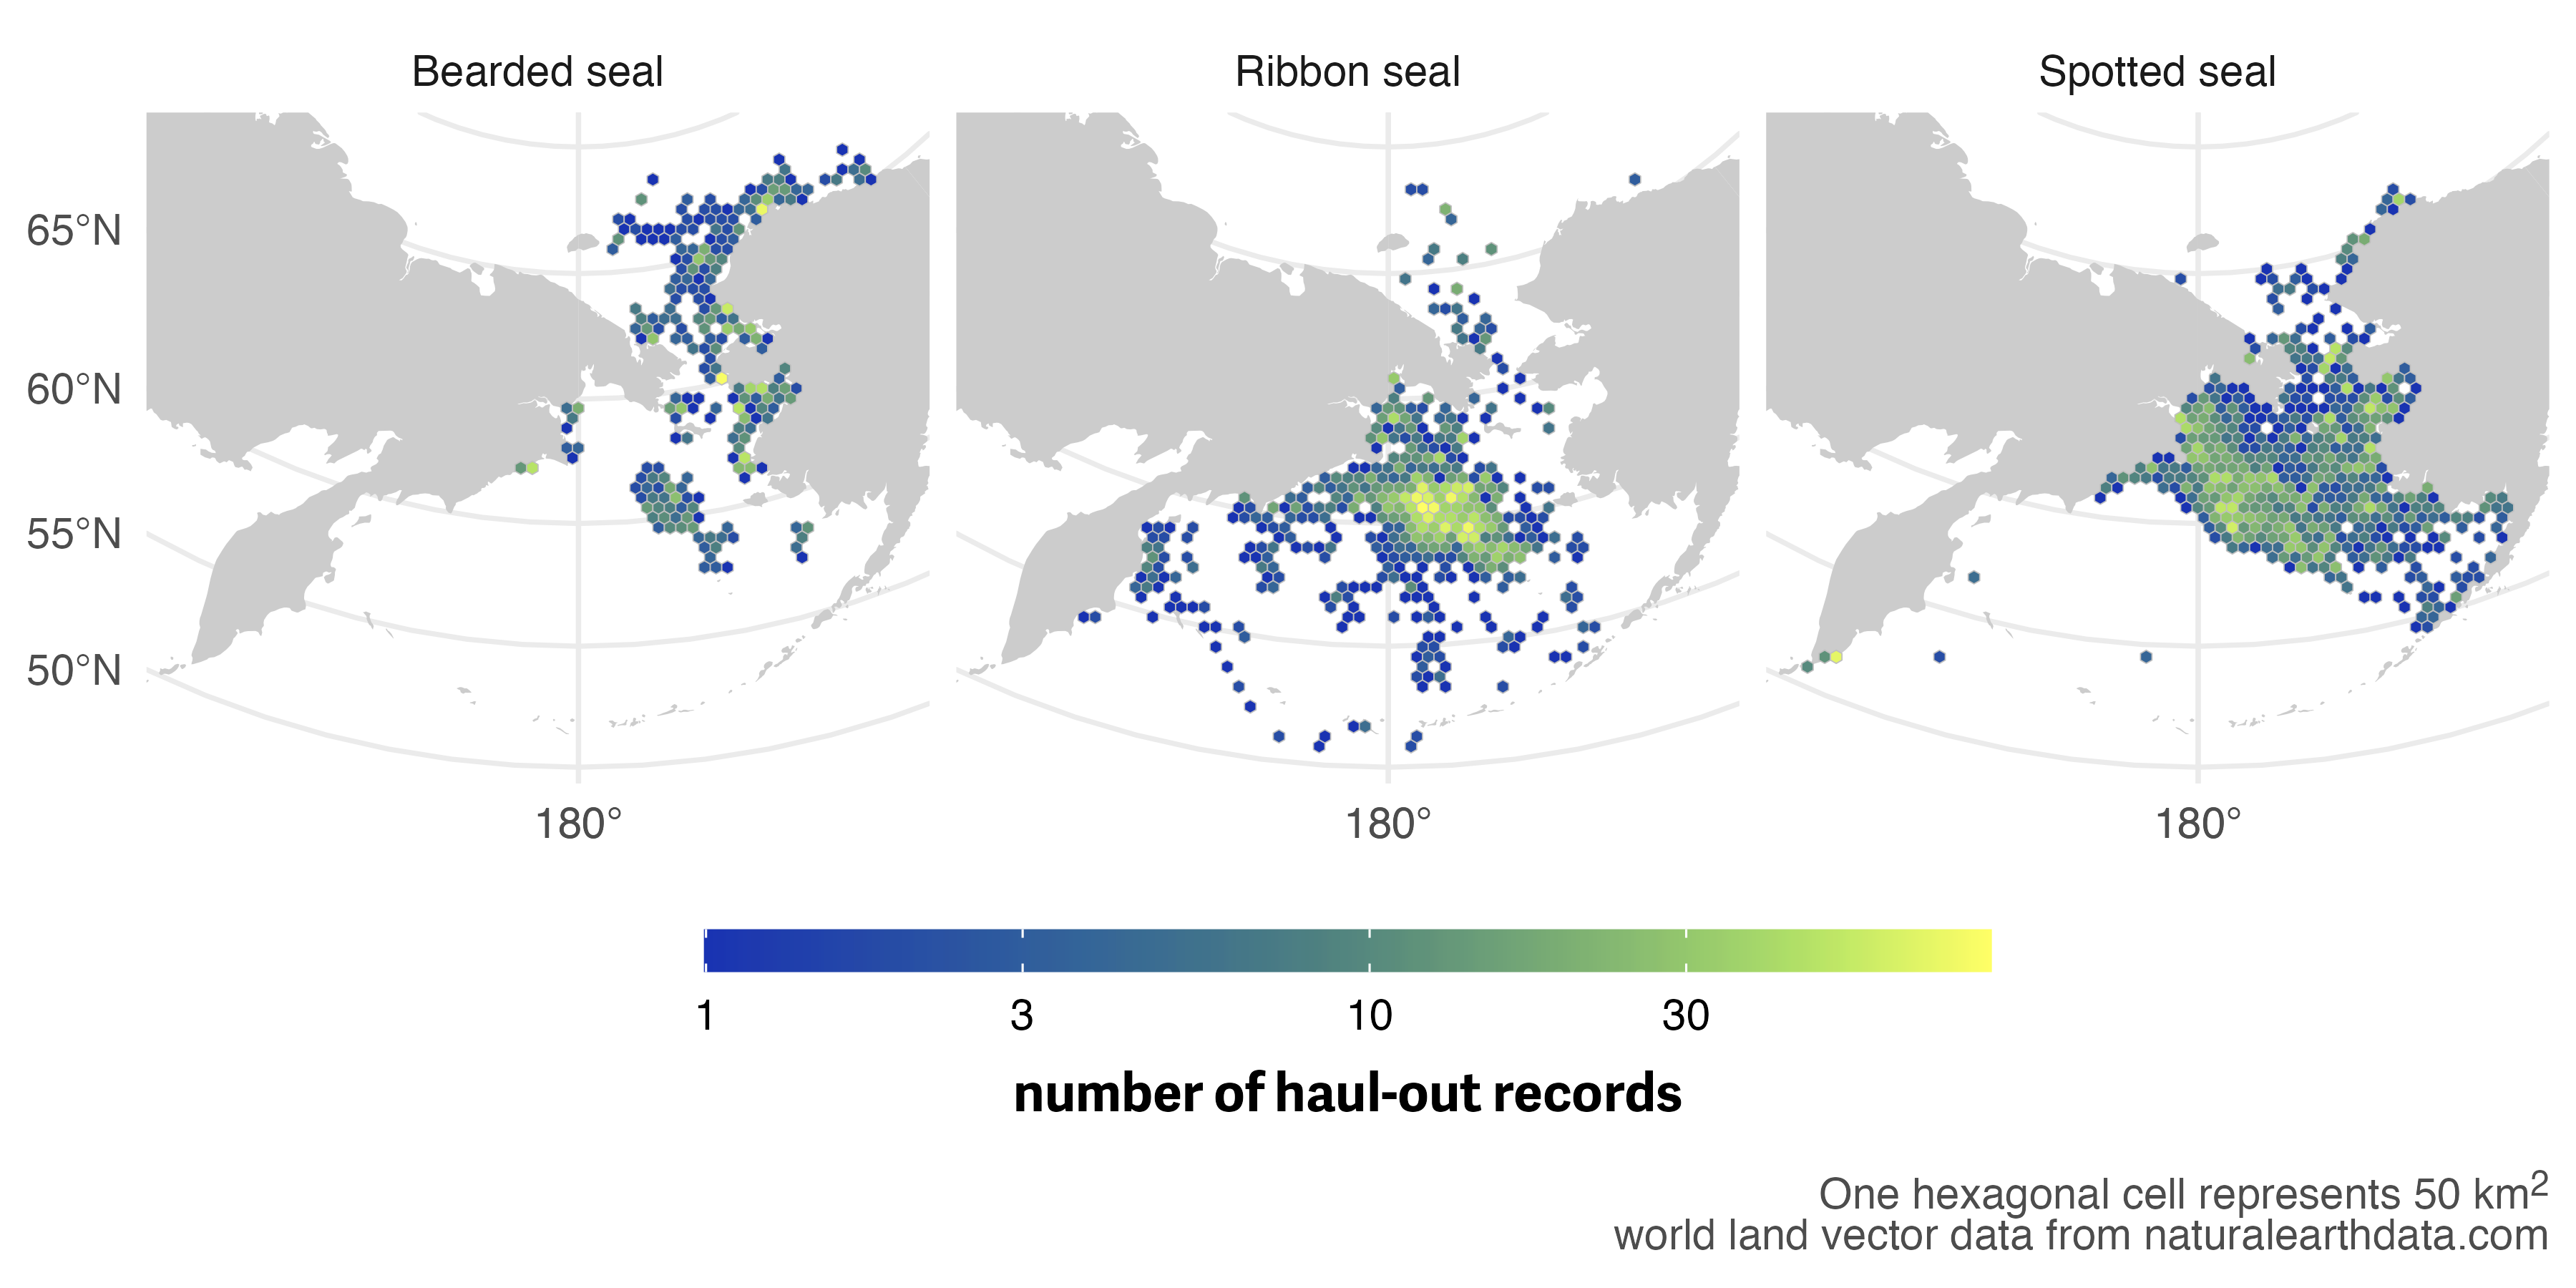
\includegraphics[width=1\linewidth]{../figures/Figure-003} \caption{\textbf{Spatial distribution of haul-out records from 1 March through July 15 for bearded, ribbon, and spotted seal.} \linebreak Linking location estimates with haul-out records in space and time allows for inclusion of weather covariates in the final model. For this visualization, data were collated across all years between 2005 and 2020 and each hexagonal cell represents an area of 50 km\textsuperscript{2}. World land vector data from \url{https://naturalearthdata.com}.}\label{fig:dataMap}
\end{figure}



\begin{figure}
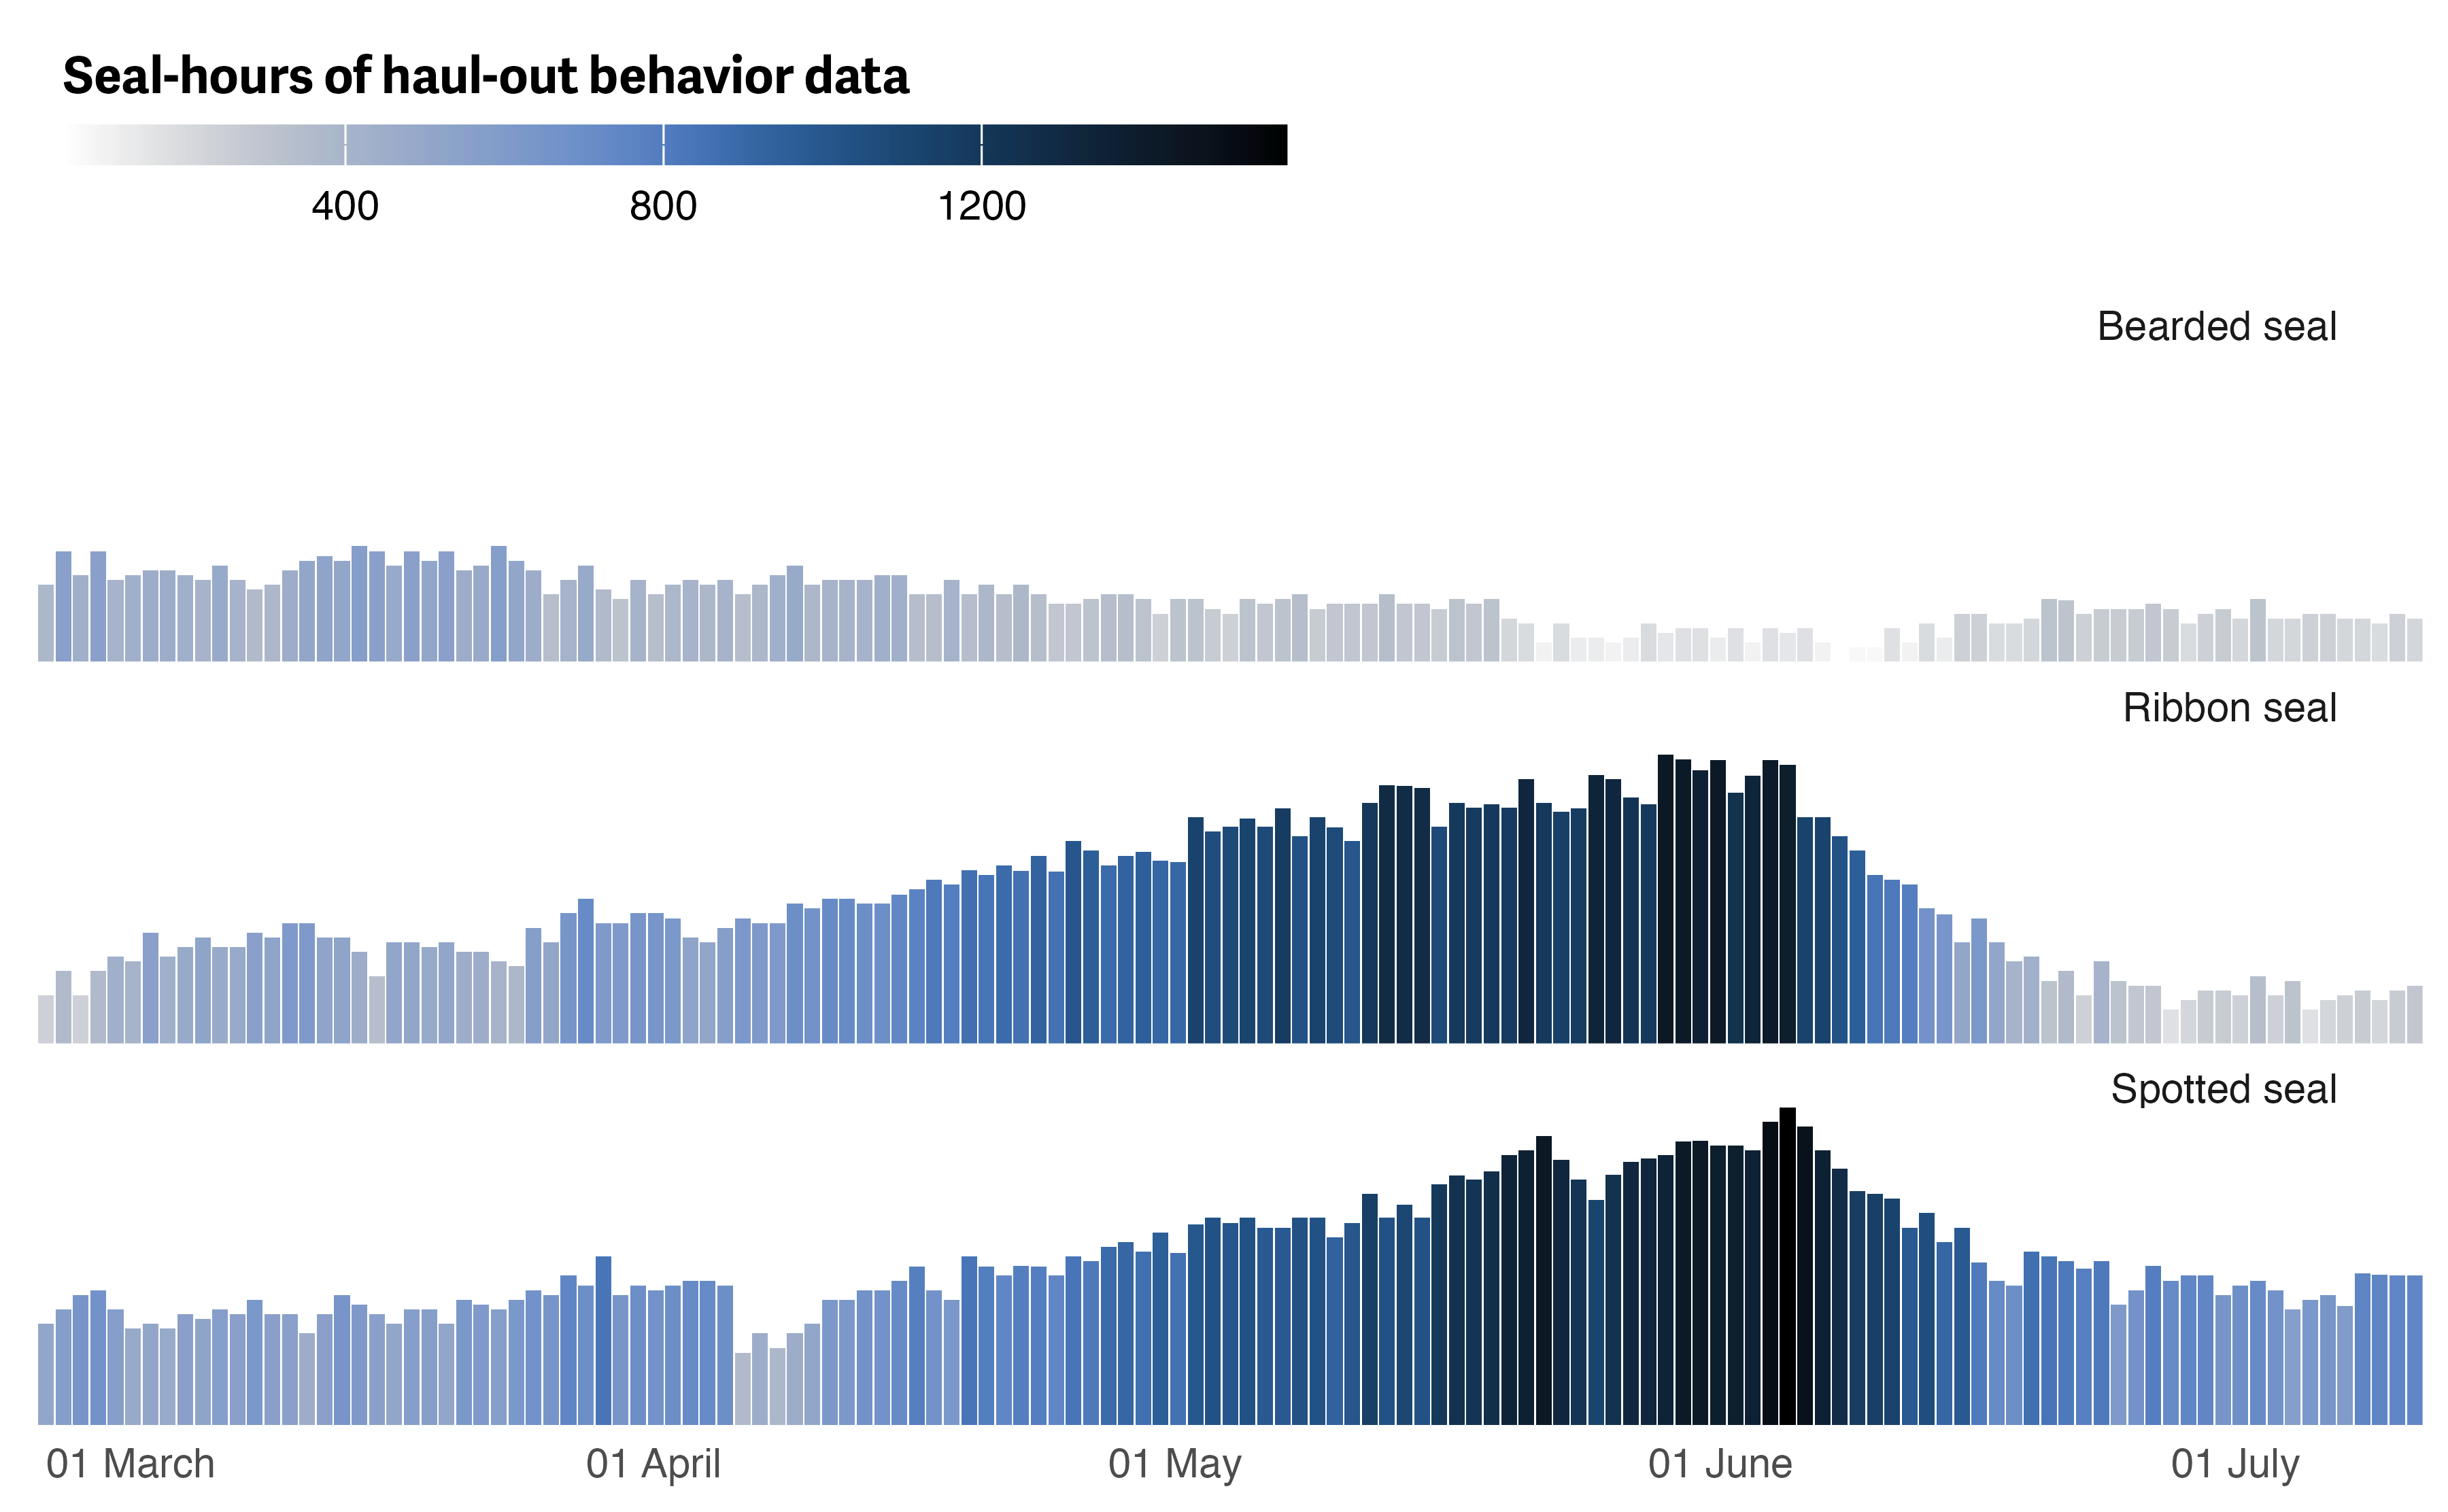
\includegraphics[width=1\linewidth]{../figures/Figure-004} \caption{\textbf{Seasonal distribution of haul-out behavior observations by species} \linebreak Distribution of hourly percent-dry bio-logger data from 1 March to 15 July for each species. Data are grouped by day-of-year and presented in seal-hours collated across all years between 2005 and 2020. Seal-hours of data are represented as a color gradient and bar height. The higher amount of data from May and June in ribbon and spotted seals coincides with peak molting when seals (and their attached bio-loggers) are more likely hauled out. Additionally, many bio-logger deployments started in April and May. The overall reduced quantity of observations from bearded seals is reflective of the lower number of bio-logger deployments in the study and the fact that the majority of deployments on bearded seals occurred in August and September; therefore most bio-loggers deployed had exhausted their batteries.}\label{fig:dataCal}
\end{figure}

Across all three seal species, generally, models omitting year effects suggested
that day-of-year, solar hour, age-sex class, temperature, and wind substantially
influenced haul-out behavior of all three species, with \(F\) tests producing
\(p\)-values less than 0.05 for variables embodying these effects and/or their
interactions. Haul-out probabilities typically increased throughout March and
April, reaching a peak in May and early June before declining again. Diurnal
patterns were present, with maximum haul-out behavior centered around local
solar noon.

\subsection*{Bearded Seals}\label{bearded-seals}
\addcontentsline{toc}{subsection}{Bearded Seals}

Age and sex class were not included in the model for bearded seals due to our
lower sample size for adult and young-of-year age classes. As such, results are
shown for all ages (Figure \ref{fig:beardedHOCal}; see also Supplemental Information Fig.
\ref{fig:beardedPredSE}). Additionally, after approximately 9 months, 7 devices
deployed on the rear flipper of bearded seals reported implausible hourly
percent-dry data (100\% dry for several weeks but indicative of movement and
increasing transmission rates (see Boveng \& Cameron (2013))). All data after the first
instance of unrealistic values were censored from this analysis. In addition to
a peak around local solar noon, the bearded seal model predicted additional
haul-out activity around local midnight. In concert with the lower magnitude of
haul-out probability, bearded seal haul-out behavior was also more protracted
throughout the spring season compared to ribbon
and spotted seals (see below). Overall, bearded seals were
less likely to haul out and had a bi-modal distribution of haul-out probability
across the day.



\begin{figure}
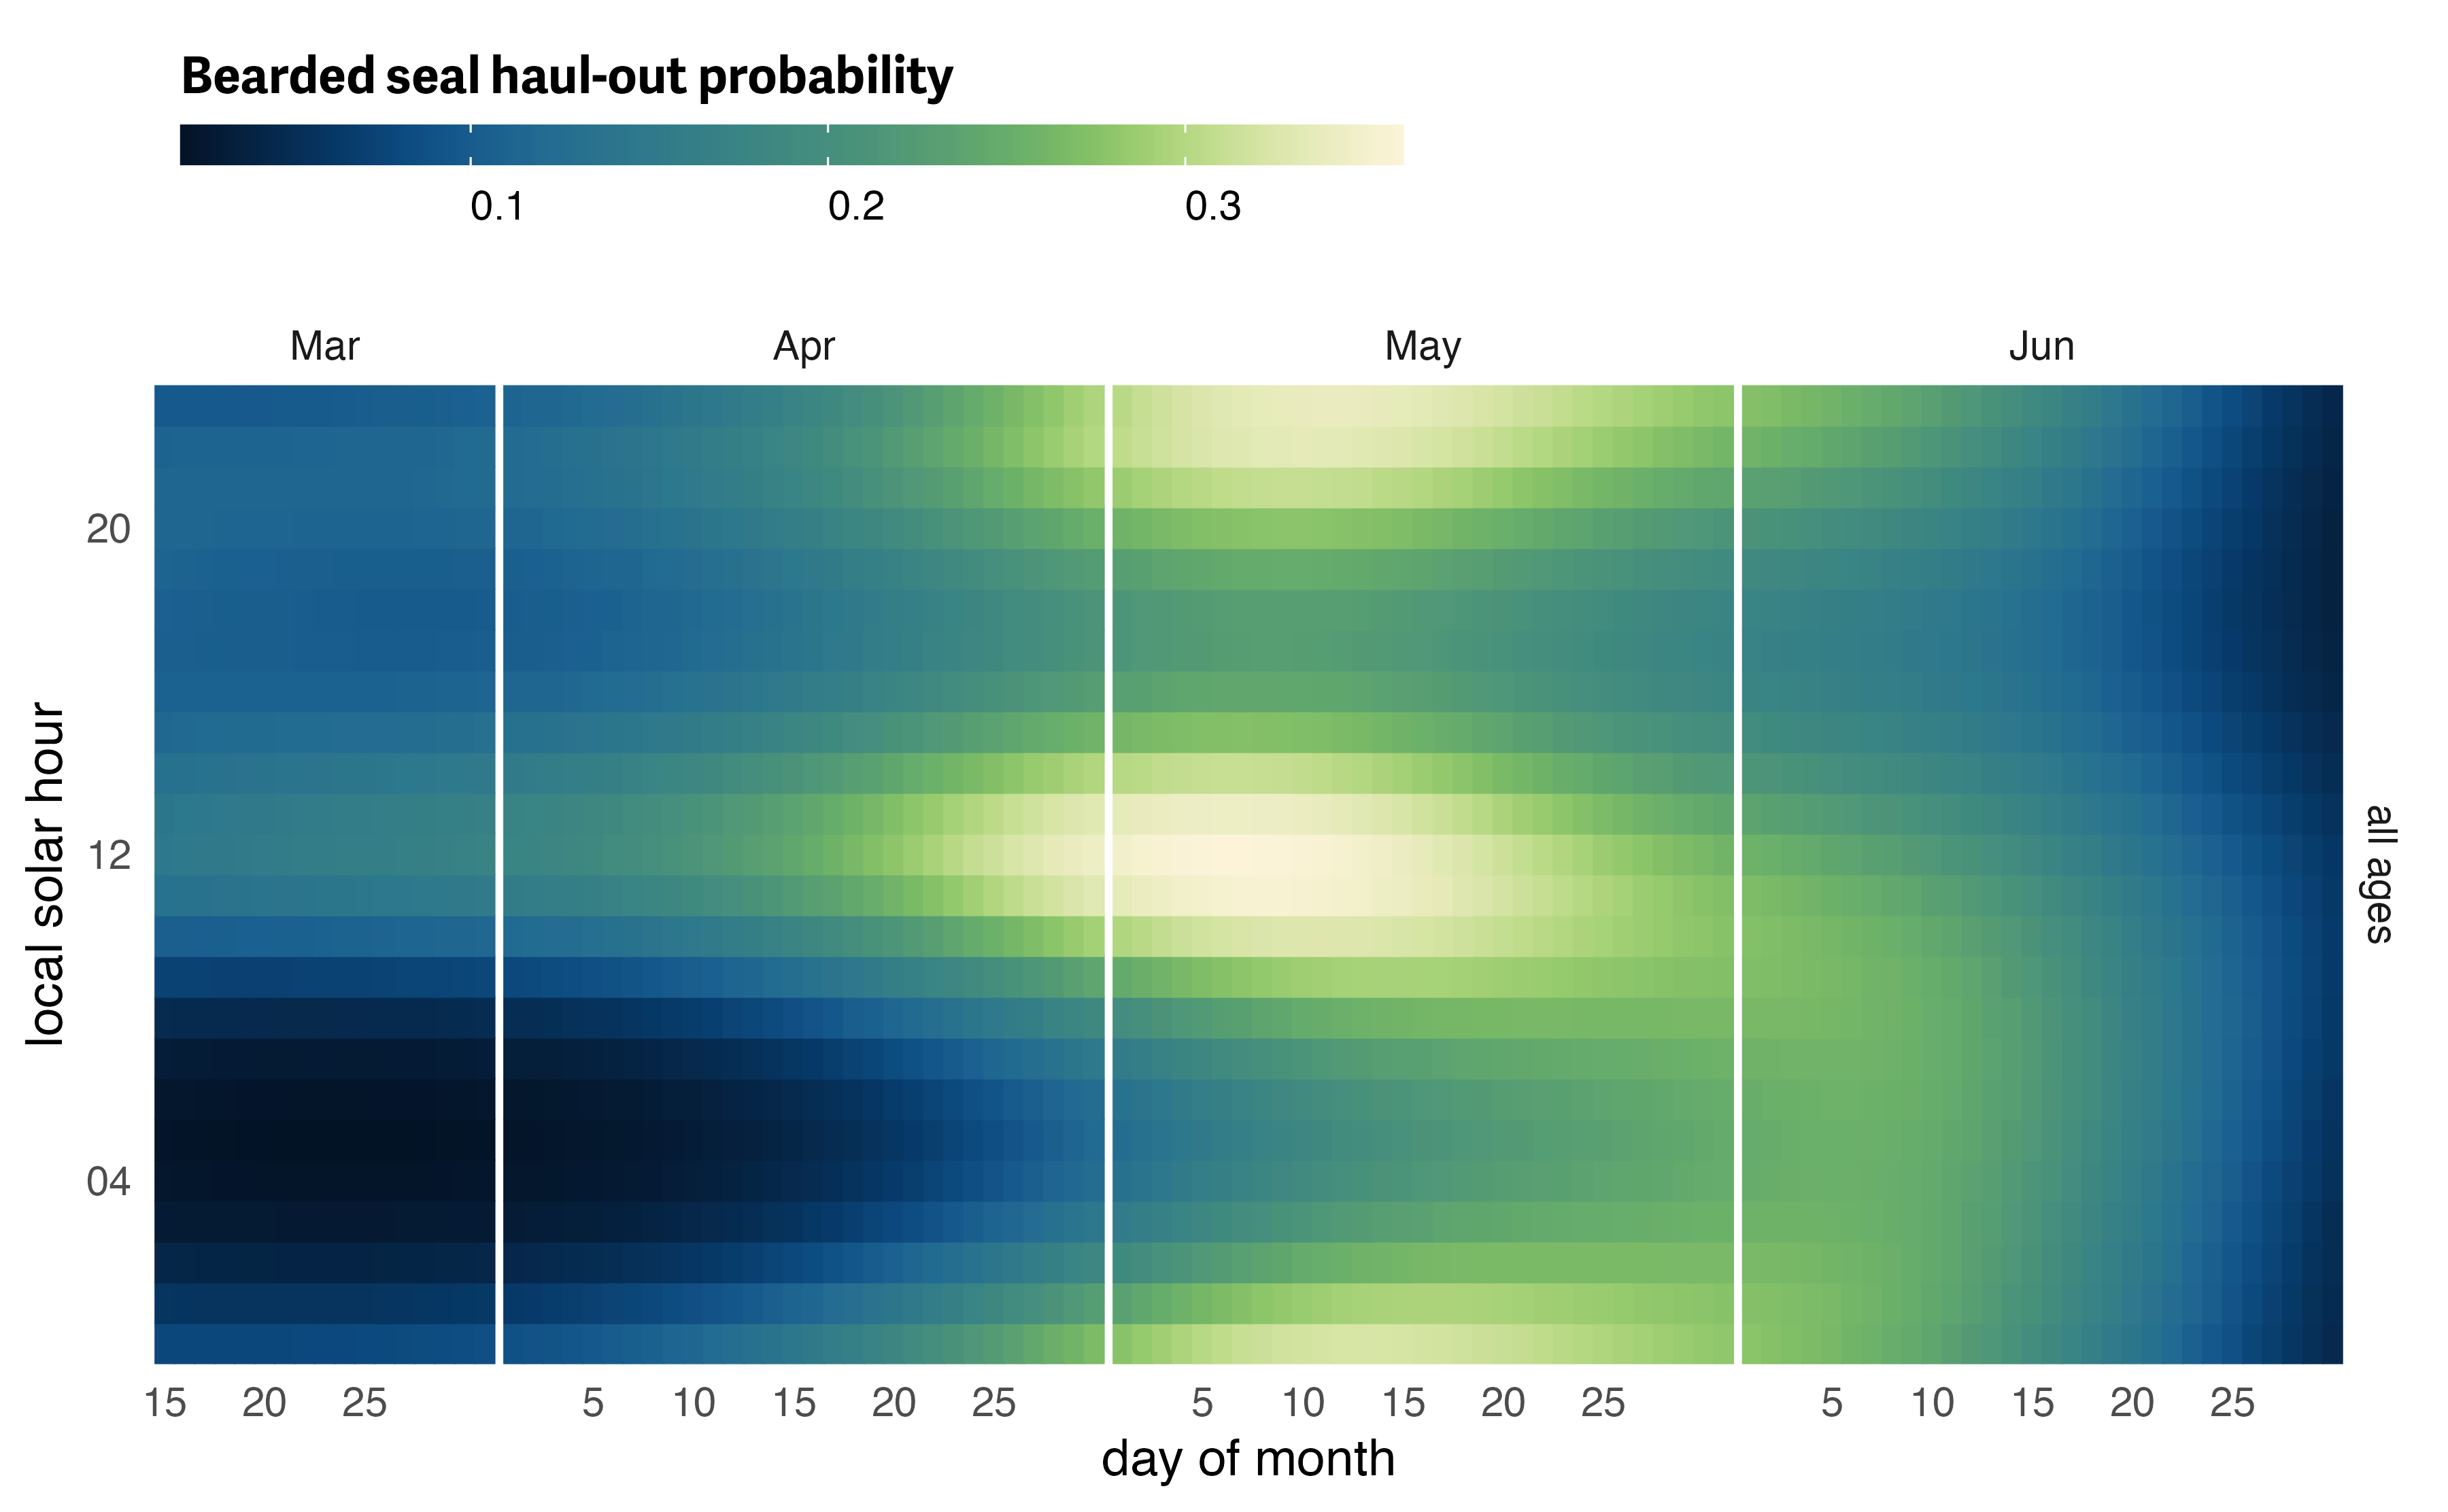
\includegraphics[width=1\linewidth]{../figures/Figure-005} \caption{\textbf{Bearded seal predicted haul-out probability} \linebreak Predicted hourly haul-out probability of bearded seals (all ages and sex classes) from 15 March to 30 June for all age and sex classes combined. Predictions in July and before 15 March were not included to avoid spurious model predictions at the edge of the data range. Weather covariate values in the prediction were based on a simple generalized additive model for each weather covariate with smooth terms for day-of-year and solar hour to account for anticipated variability within a day over the season. Note, our model predicts lower haul-out probability for bearded seals overall compared to ribbon and spotted seals and the color scales are not directly comparable.}\label{fig:beardedHOCal}
\end{figure}

When exploring the influence of weather, bearded seal haul-out probability
was strongly affected by wind
(\(F_{1,42728}\)
= 130.468; \(p\) = \textless0.001)
and temperature
(\(F_{1,42728}\)
= 19.5; \(p\) =
\textless0.001) with much higher haul-out probability during
periods of higher temperatures and low wind speeds (Figure \ref{fig:beardedHOwx}).
Not surprisingly, wind chill
(\(F_{1,42728}\)
= 14.54; \(p\) =
\textless0.001) was also important. Barometric
pressure (\(F_{1,42728}\)
= 7.779; \(p\) =
0.005) was also significant factor although less
apparent (Figure \ref{fig:beardedHOwx}). Any effect of precipitation
was not a significant influence on haul-out probability
(\(F_{1,42728}\)
= 0.519; \(p\) =
0.471).



\begin{figure}
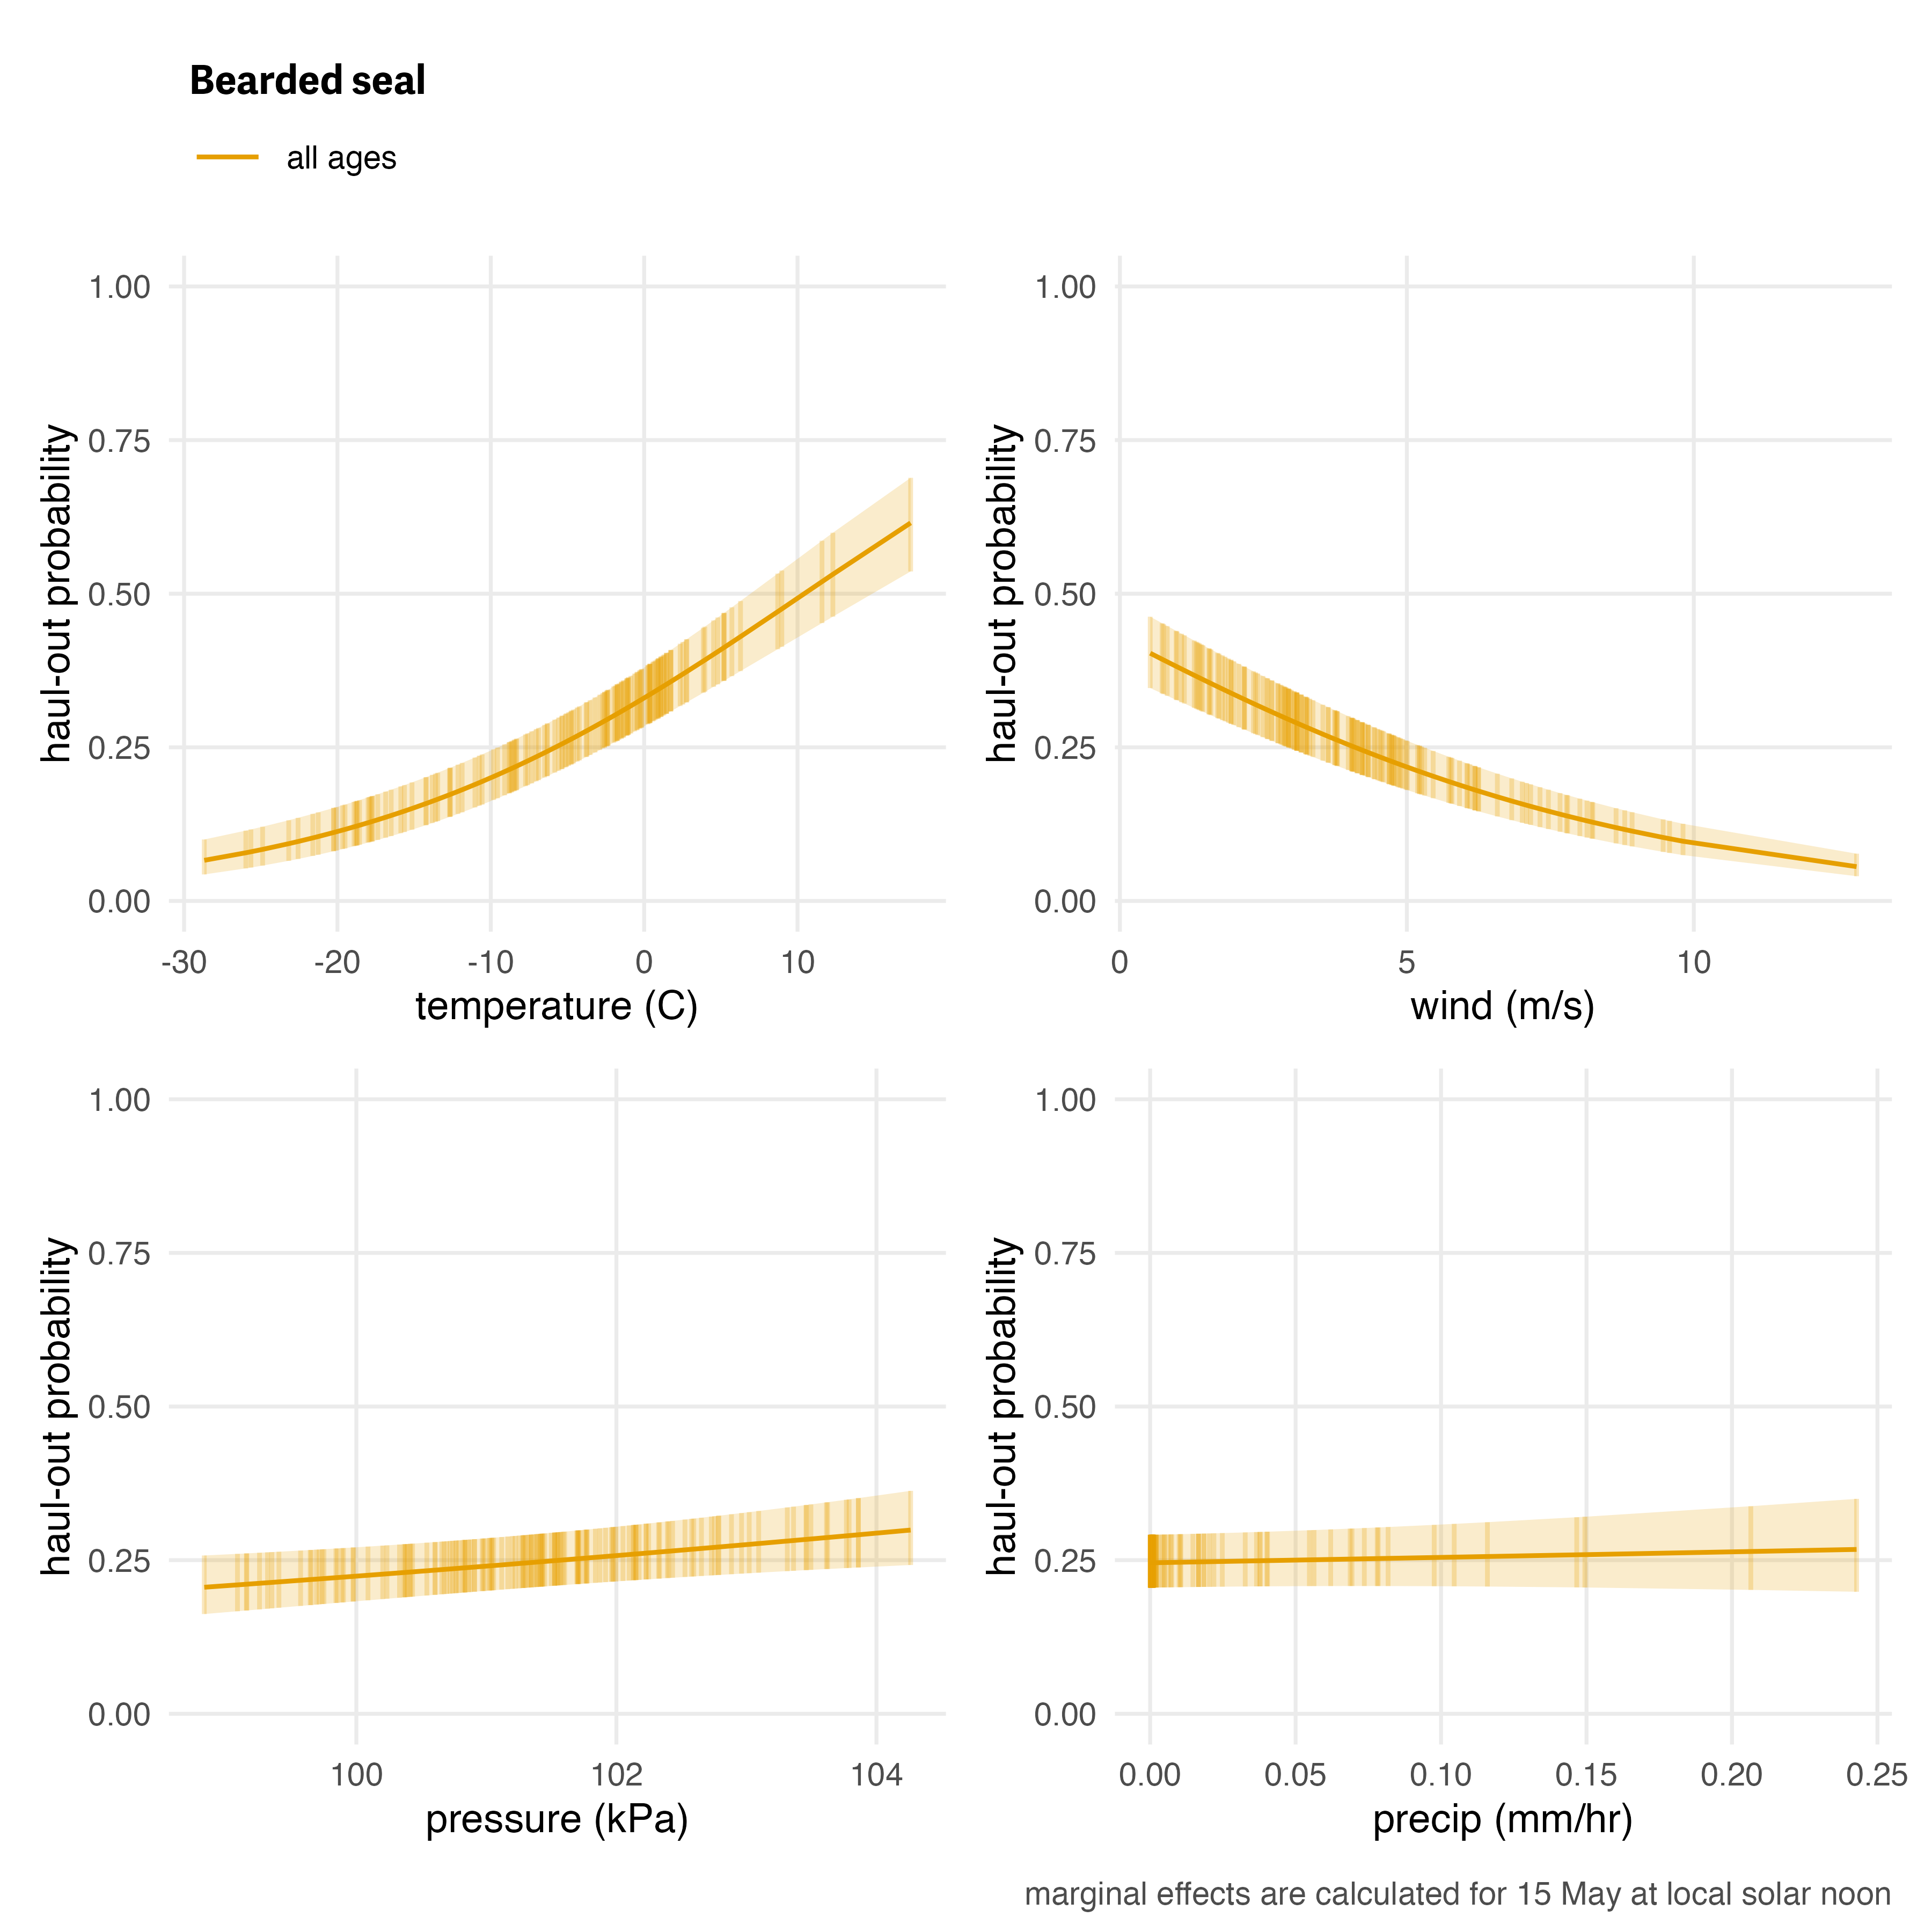
\includegraphics[width=1\linewidth]{../figures/Figure-006} \caption{\textbf{Influence of weather covariates on bearded seal haul-out probability} \linebreak Marginal effects of temperature, wind, barometric pressure, and precipitation on the predicted haul-out probability of bearded seals combined across all age and sex classifications. Hour of the day was fixed at local solar noon and day-of-year fixed at 15 May. The other weather covariate values were predicted from a simple generalized additive model for each weather covariate with smooth terms for day-of-year and solar hour to account for anticipated variability within a day over the season. While the marginal effect of the covariate is continuous, points and vertical lines representing the 95\% confidence interval around the predicted haul-out probability are shown only at observed weather values to give an indication of how the observations are distributed across the range of weather values.}\label{fig:beardedHOwx}
\end{figure}

\subsection*{Ribbon Seals}\label{ribbon-seals}
\addcontentsline{toc}{subsection}{Ribbon Seals}

Ribbon seals exhibited a pattern of gradually increasing haul-out probability in
April that peaks in late May for subadults and in early June for adults (Figure
\ref{fig:ribbonHOCal}; see also Supplemental Information Fig.
\ref{fig:ribbonPredSE}). There is an apparent seasonal progression with
subadults hauling out earlier in the season followed by adult males and, then,
adult females. Haul-out behavior was clearly centered around local solar noon
and expanded to other hours later in the spring as seals entered their molting
period. Subadults showed an earlier start and more intense haul-out activity in
April and May. The young-of-the-year records began after weaning and the model
predictions seemed to indicate development of in-water activities (e.g.
swimming, foraging) in May and, like adults, haul-out behavior was centered
around solar noon. Adult females had a more protracted haul-out season compared
to males, and more time was spent hauled out in June compared to adult males and
subadults.



\begin{figure}
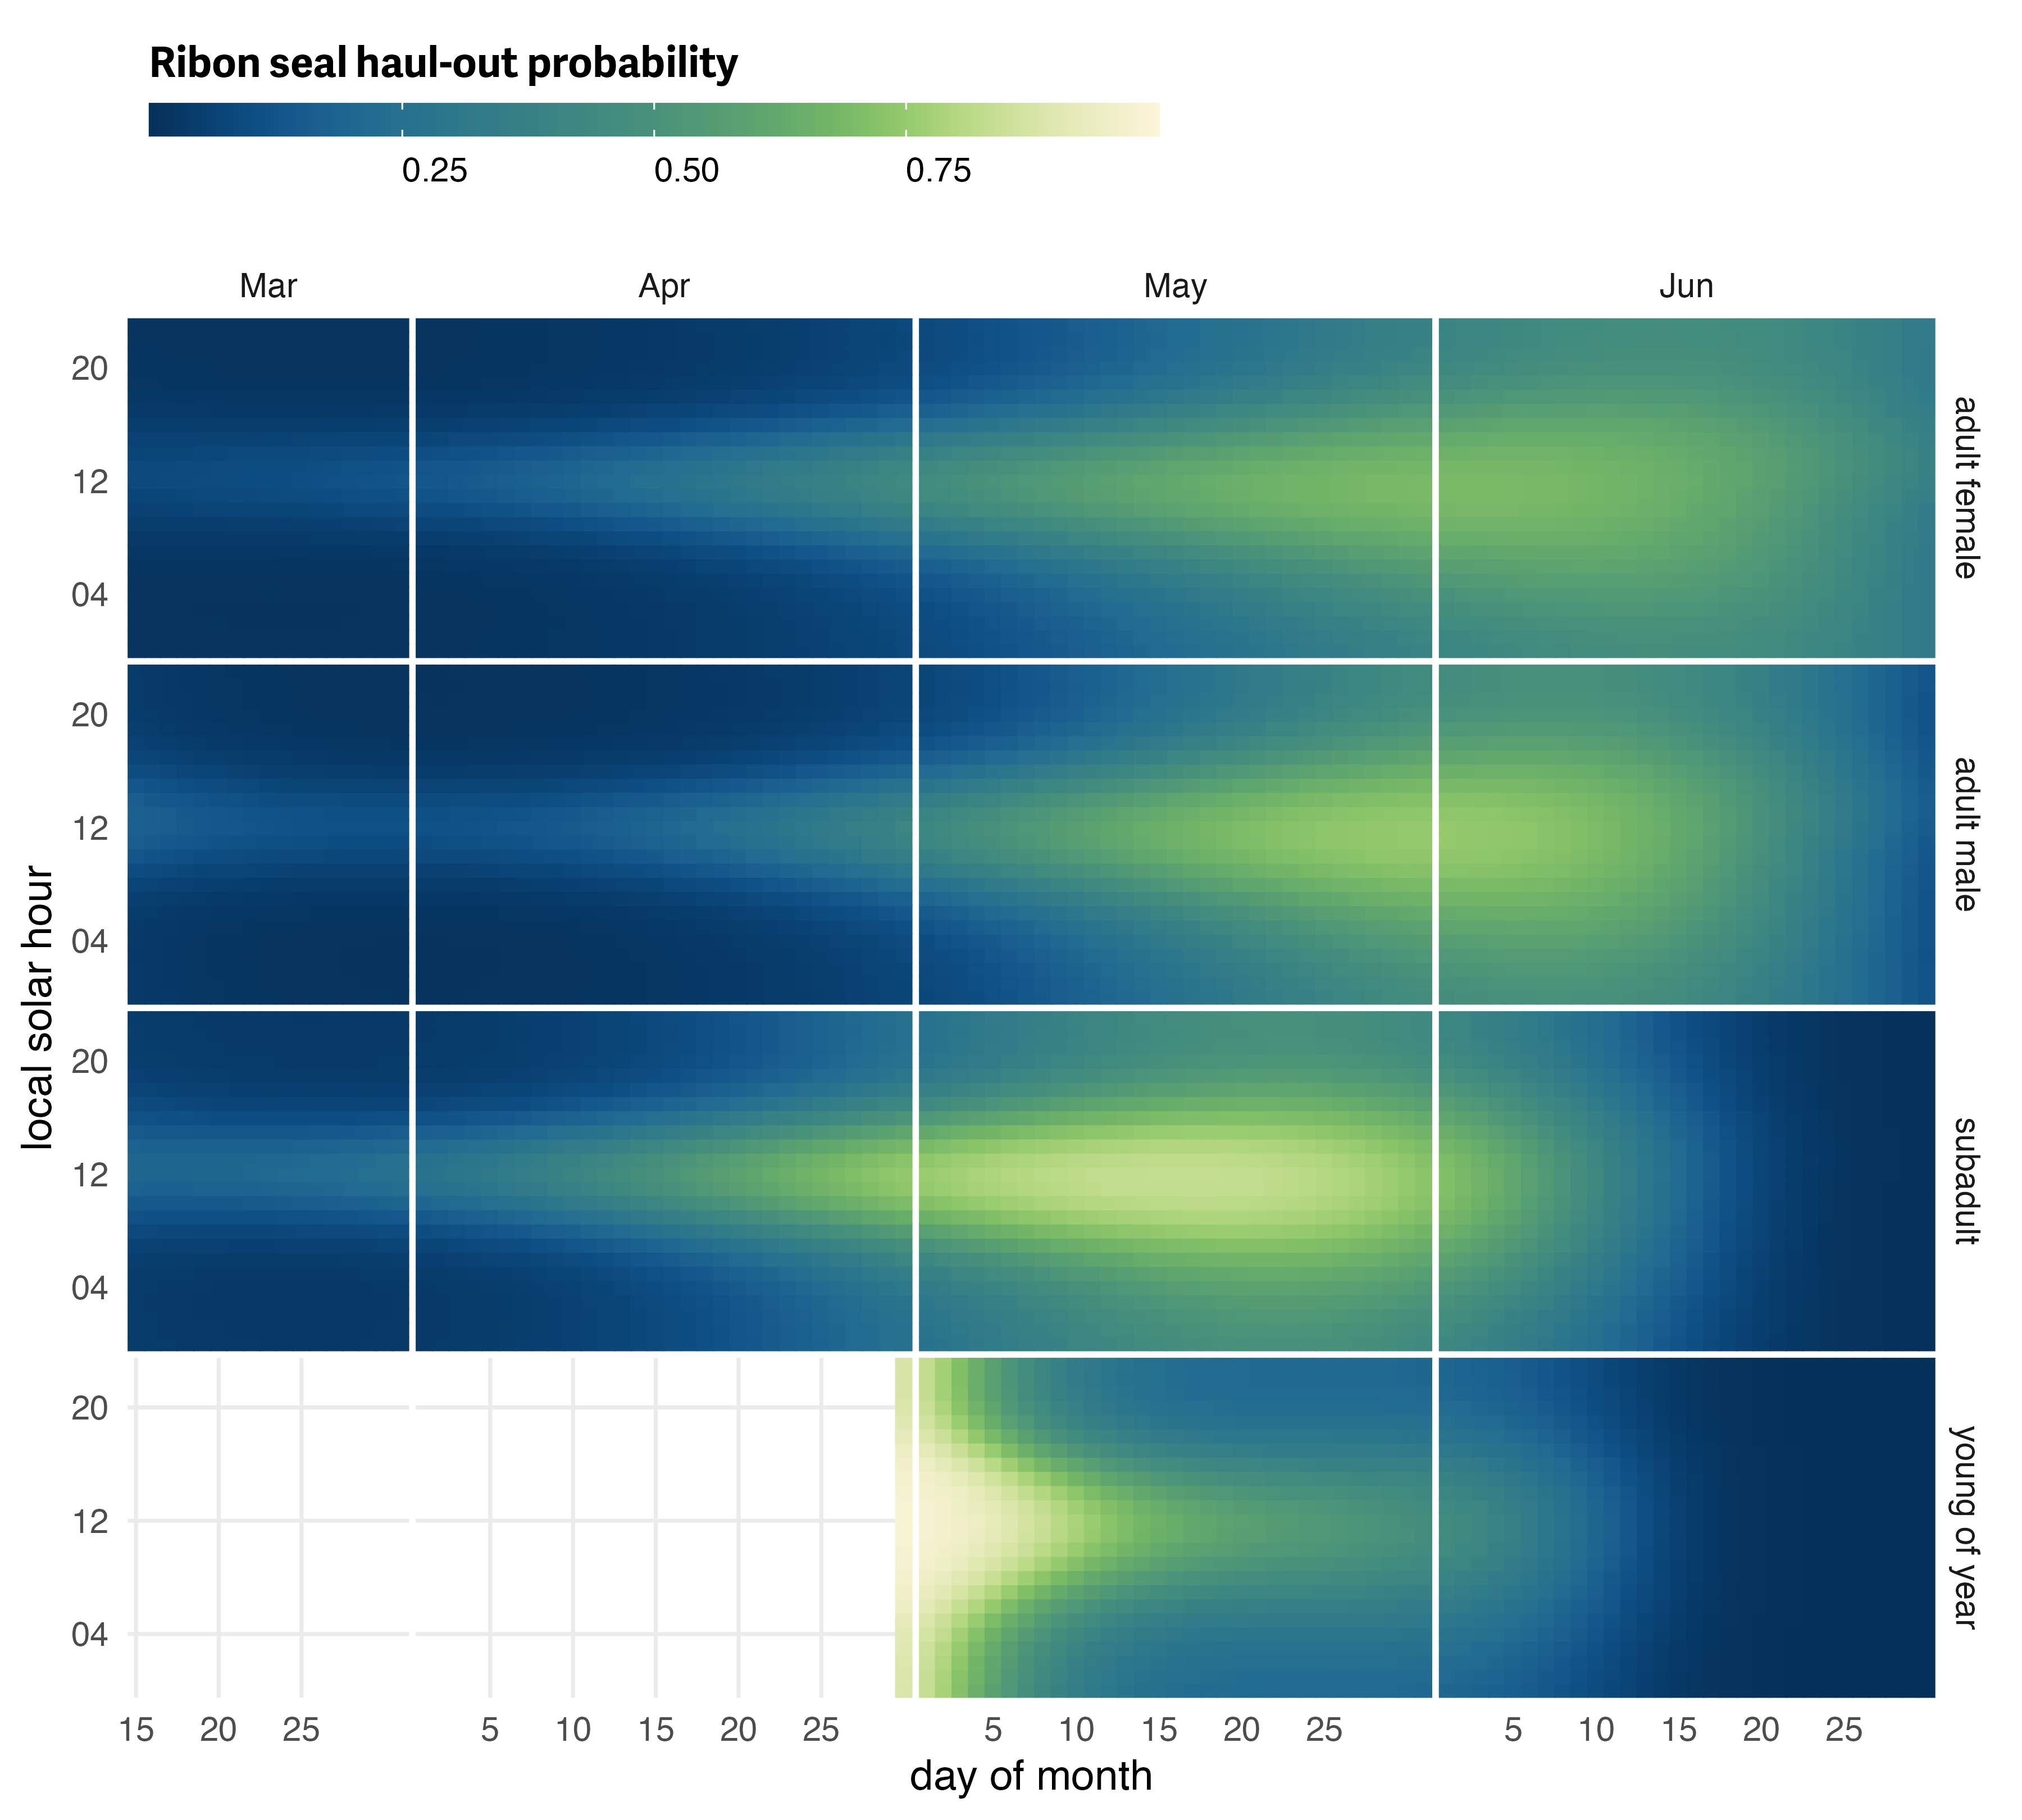
\includegraphics[width=1\linewidth]{../figures/Figure-007} \caption{\textbf{Ribbon seal predicted haul-out probability} \linebreak Predicted hourly haul-out probability of ribbon seals from 15 March to 30 June for each age and sex class used in the model. Weather covariate values in the prediction were based on a simple generalized additive model for each weather covariate with smooth terms for day-of-year and solar hour to account for anticipated variability within a day over the season. Predictions for young of the year show their transition from newly weaned pups resting on the ice to more in-water activities. Predictions in July and before 15 March were not included to avoid spurious model predictions at the edge of the data range.}\label{fig:ribbonHOCal}
\end{figure}

The haul-out probability for ribbon seals was mostly influenced by
temperature
(\(F_{1,99540}\)
= 6.87; \(p\) = 0.009) and wind
(\(F_{1,99540}\)
= 49.314; \(p\) = \textless0.001) with barometric pressure
(\(F_{1,99540}\)
= 3.446; \(p\) =
0.063) having a milder impact.
Ribbon seals were more likely to haul out when temperatures were
relatively warm and less likely to haul out at higher winds and lower pressure
values (Figure \ref{fig:ribbonHOwx}). Neither wind chill
(\(F_{1,99540}\)
= 1.83; \(p\) =
0.176) nor precipitation
(\(F_{1,99540}\)
= 0; \(p\) =
0.989) were a significant
influence on haul-out probability. Compared with bearded seals, the effect of
weather covariates on the predicted haul-out probability for
ribbon seals was less striking. Because our ribbon seal model included age and sex class, we can
visualize the different influences of weather covariates on those classes and see
that subadults differ from adult males and females (Figure \ref{fig:ribbonHOwx}).



\begin{figure}
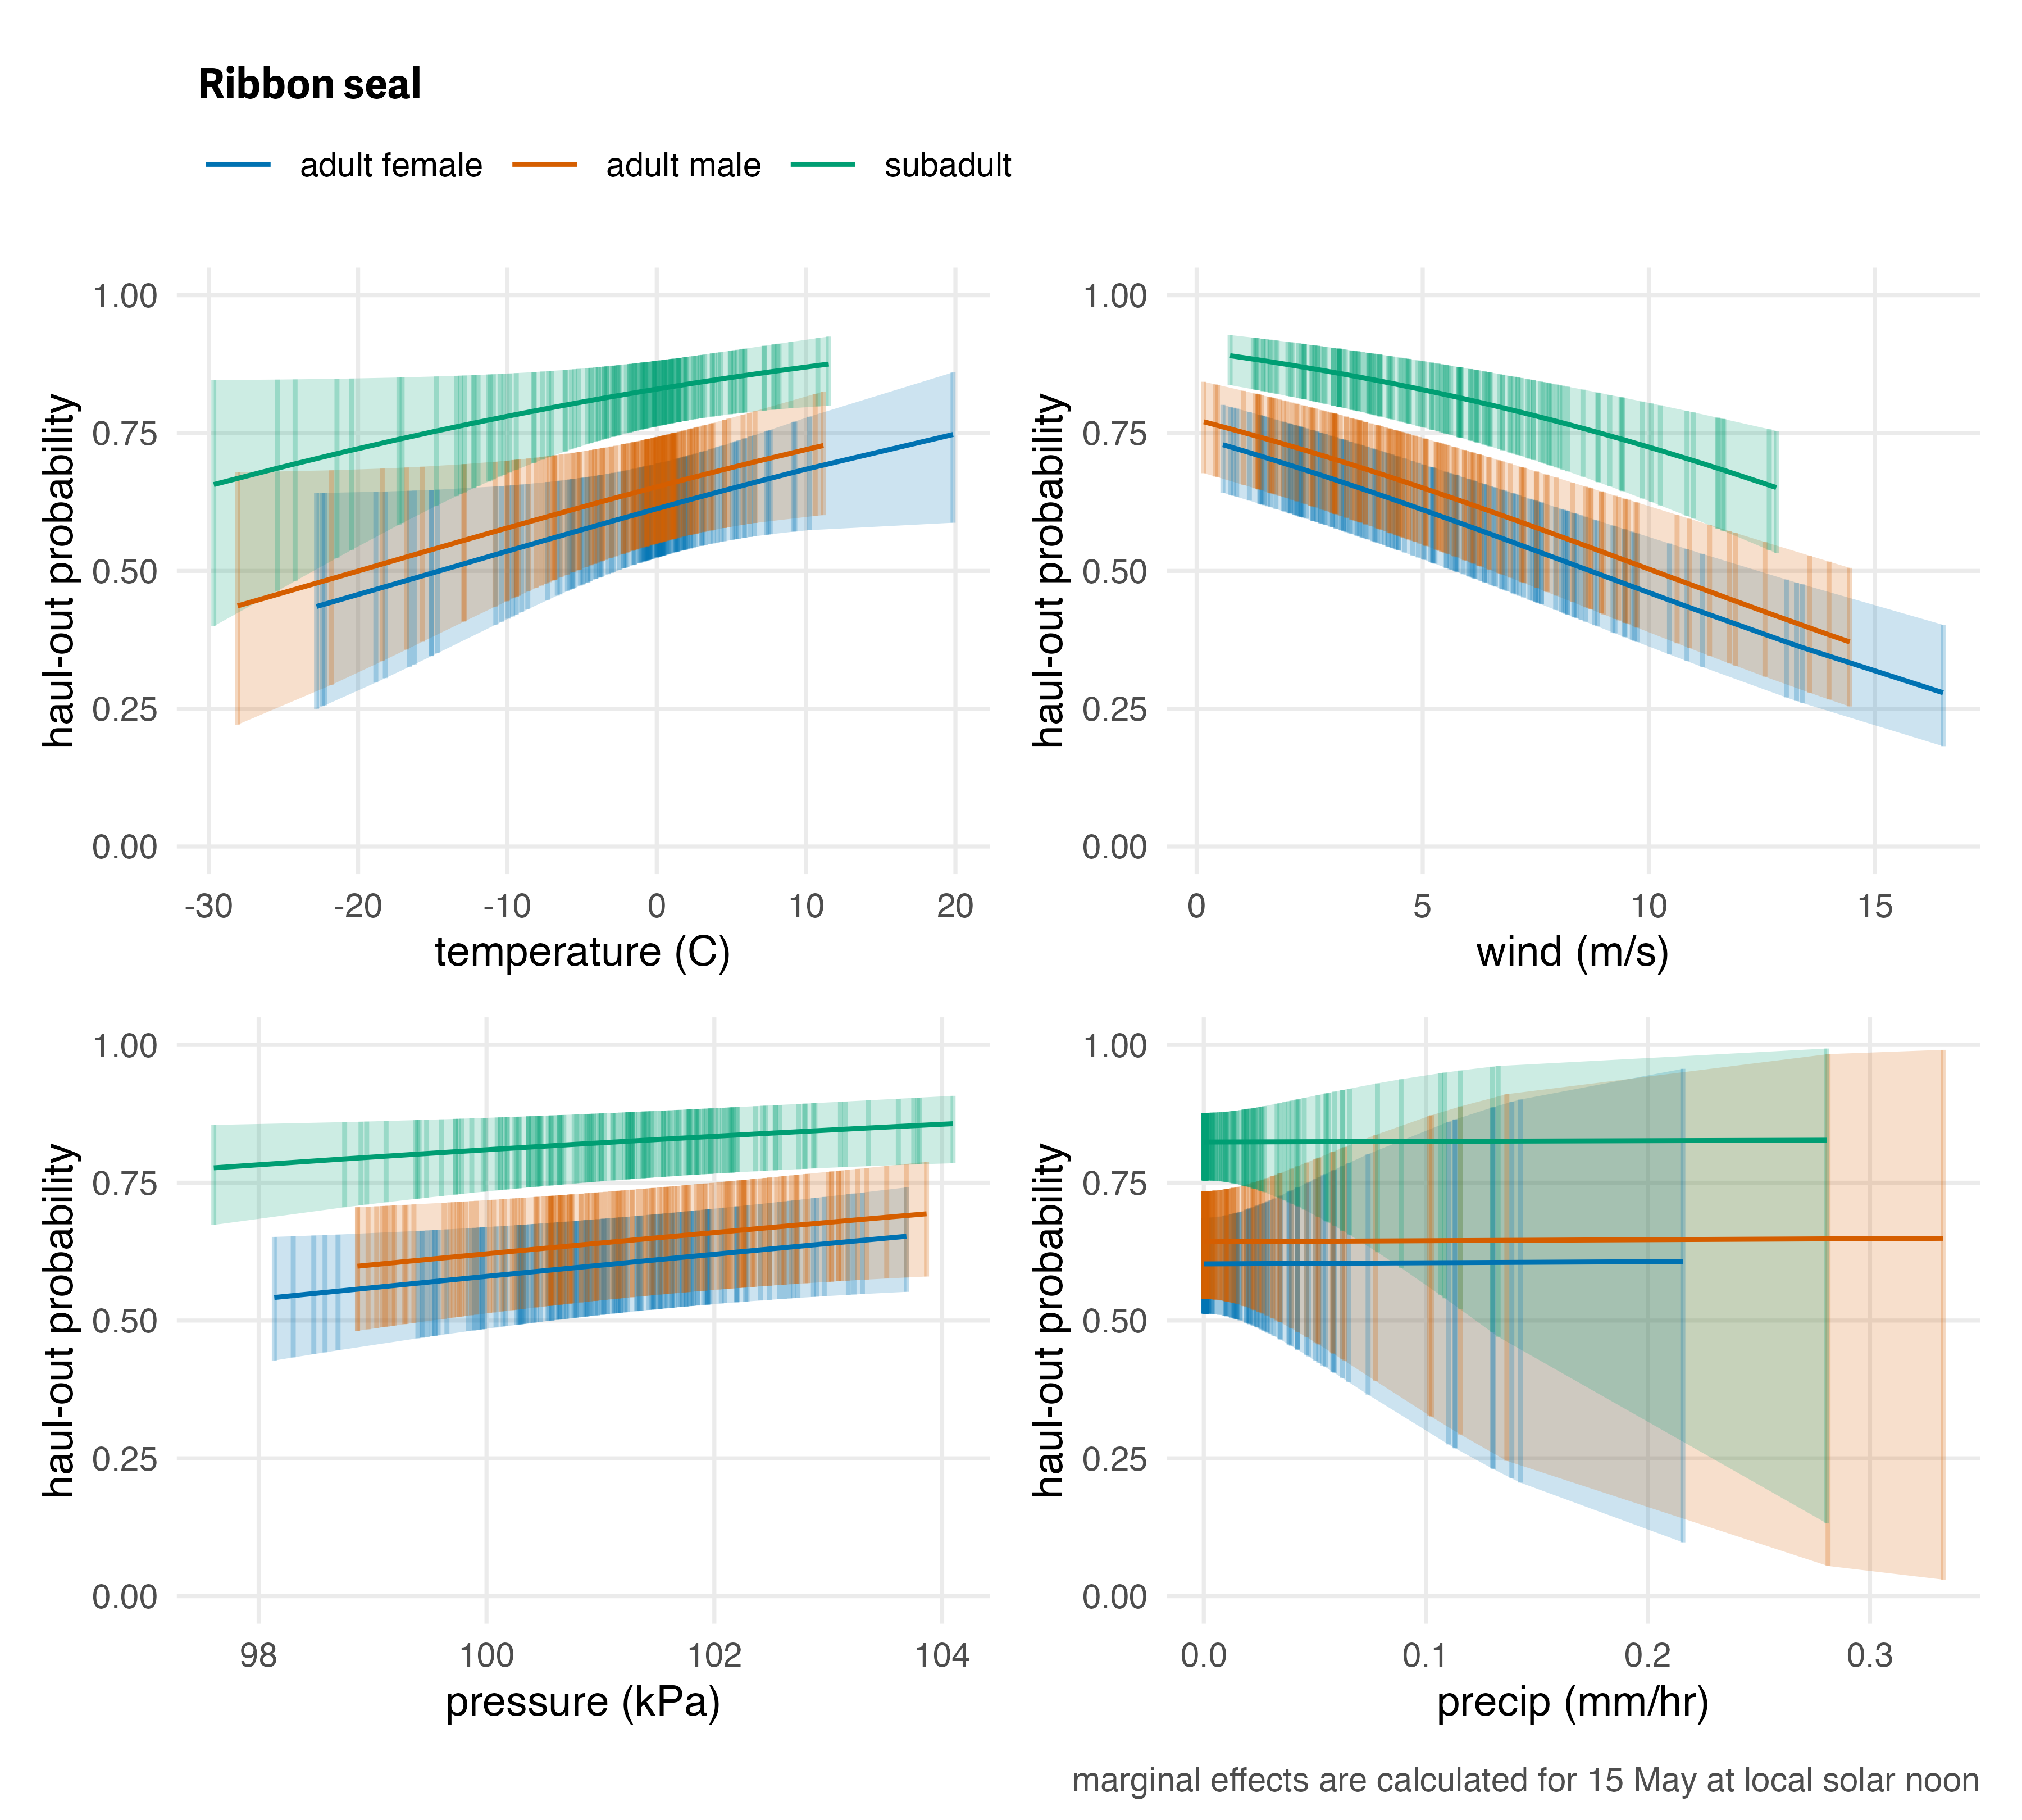
\includegraphics[width=1\linewidth]{../figures/Figure-008} \caption{\textbf{Influence of weather covariates on ribbon seal haul-out probability} \linebreak Marginal effects of temperature, wind, barometric pressure, and precipitation on the predicted haul-out probability of ribbon seals within each age and sex classifications. Hour of the day was fixed at local solar noon and day-of-year fixed at 15 May. The other weather covariate values were predicted from a simple generalized additive model for each weather covariate with smooth terms for day-of-year and solar hour to account for anticipated variability within a day over the season. While the marginal effect of the covariate is continuous, points and vertical lines representing the 95\% confidence interval around the predicted haul-out probability are shown only at observed weather values to give an indication of how the observations are distributed across the range of weather values.}\label{fig:ribbonHOwx}
\end{figure}

\subsection*{Spotted Seals}\label{spotted-seals}
\addcontentsline{toc}{subsection}{Spotted Seals}

Compared to ribbon seals, spotted seals showed a longer spring haul-out season
that was less intensely centered on solar noon (Figure \ref{fig:spottedHOCal};
see also Supplemental Information Fig.\ref{fig:spottedPredSE}). Adults of both
sexes spent considerable time in April, May and June hauled out. Adult spotted
seal males had a more protracted haul-out season compared to females, and more
time out of the water in June (Figure \ref{fig:spottedHOCal}). This likely
reflects the triad behavior in spotted seals when suitor males haul out with
nursing females. As with ribbon seals, the young-of-the-year records began after
weaning and the model predictions reflected development of in-water activities
(e.g.~swimming, foraging) in May and haul-out behavior centered around solar
noon.



\begin{figure}
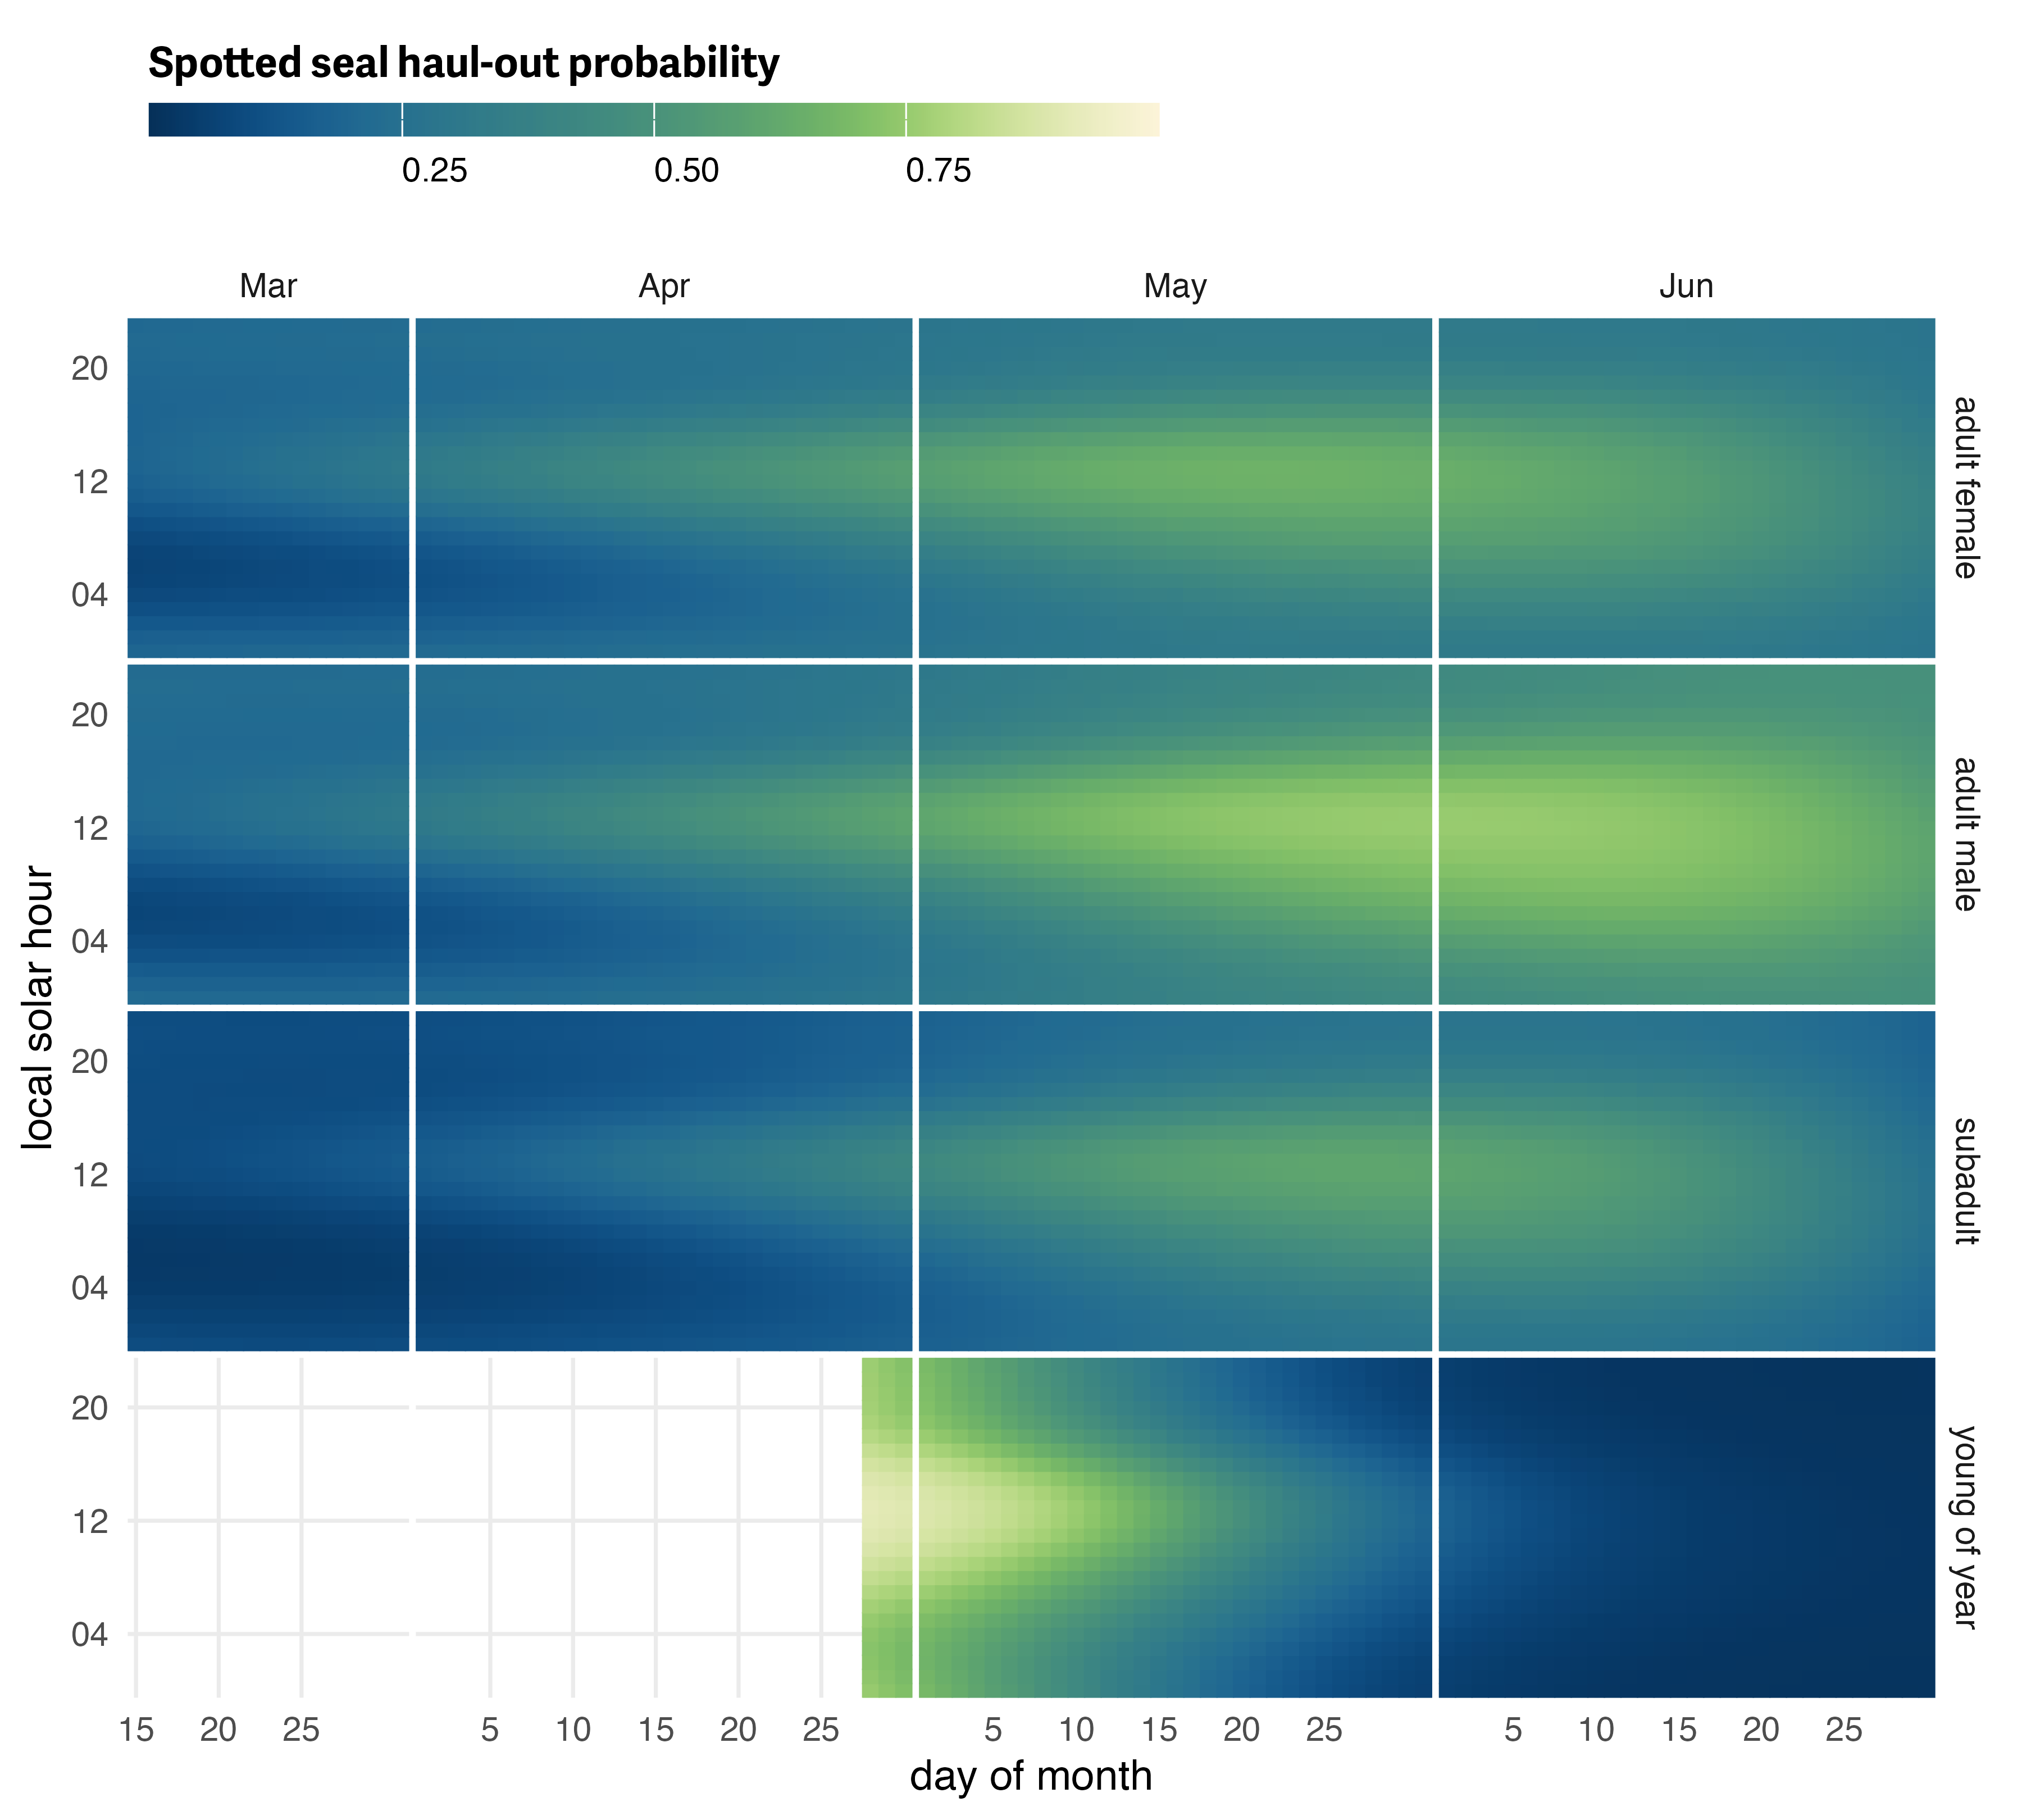
\includegraphics[width=1\linewidth]{../figures/Figure-009} \caption{\textbf{Spotted seal predicted haul-out probability} \linebreak Predicted hourly haul-out probability of spotted seals from 1 March to 30 June for each age and sex class used in the model. Weather covariate values in the prediction were based on a simple generalized additive model for each weather covariate with smooth terms for day-of-year and solar hour to account for anticipated variability within a day over the season. As with ribbon seals, predictions for young of the year show their transition from newly weaned pups resting on the ice to more in-water activities. Predictions in July and before 15 March were not included to avoid spurious model predictions at the edge of the data range.}\label{fig:spottedHOCal}
\end{figure}

Spotted seal haul-out behavior was less affected by the weather covariates
compared to ribbon and bearded seals but their influence on the model was still
significant in some cases.
Temperature
(\(F_{1,115189}\)
= 5.384; \(p\) = 0.020), wind
(\(F_{1,115189}\)
= 45.718; \(p\) = \textless0.001),
and barometric pressure
(\(F_{1,115189}\)
= 9.445; \(p\) =
0.002) were all significant. Spotted seals were more likely to be on the ice when
temperatures were relatively warm and less likely to
haul out at higher wind speeds. Wind chill
(\(F_{1,115189}\)
= 0.72; \(p\) =
0.396) and
precipitation
(\(F_{1,115189}\)
= 0.773; \(p\) =
0.379)
were not as influential as the other covariates.
Differences in the magnitude of response between the age-sex classes were
present and consistent across each of the weather covariates (Figure
\ref{fig:spottedHOwx}). There was a consistent ranking of adult males being the most
likely to haul out, followed by adult females, and, then, subadults. This differs
from ribbon seals which showed more overlap between adult males and adult females
and that subadults were most likely to haul out across the presented range of weather
covariates.



\begin{figure}
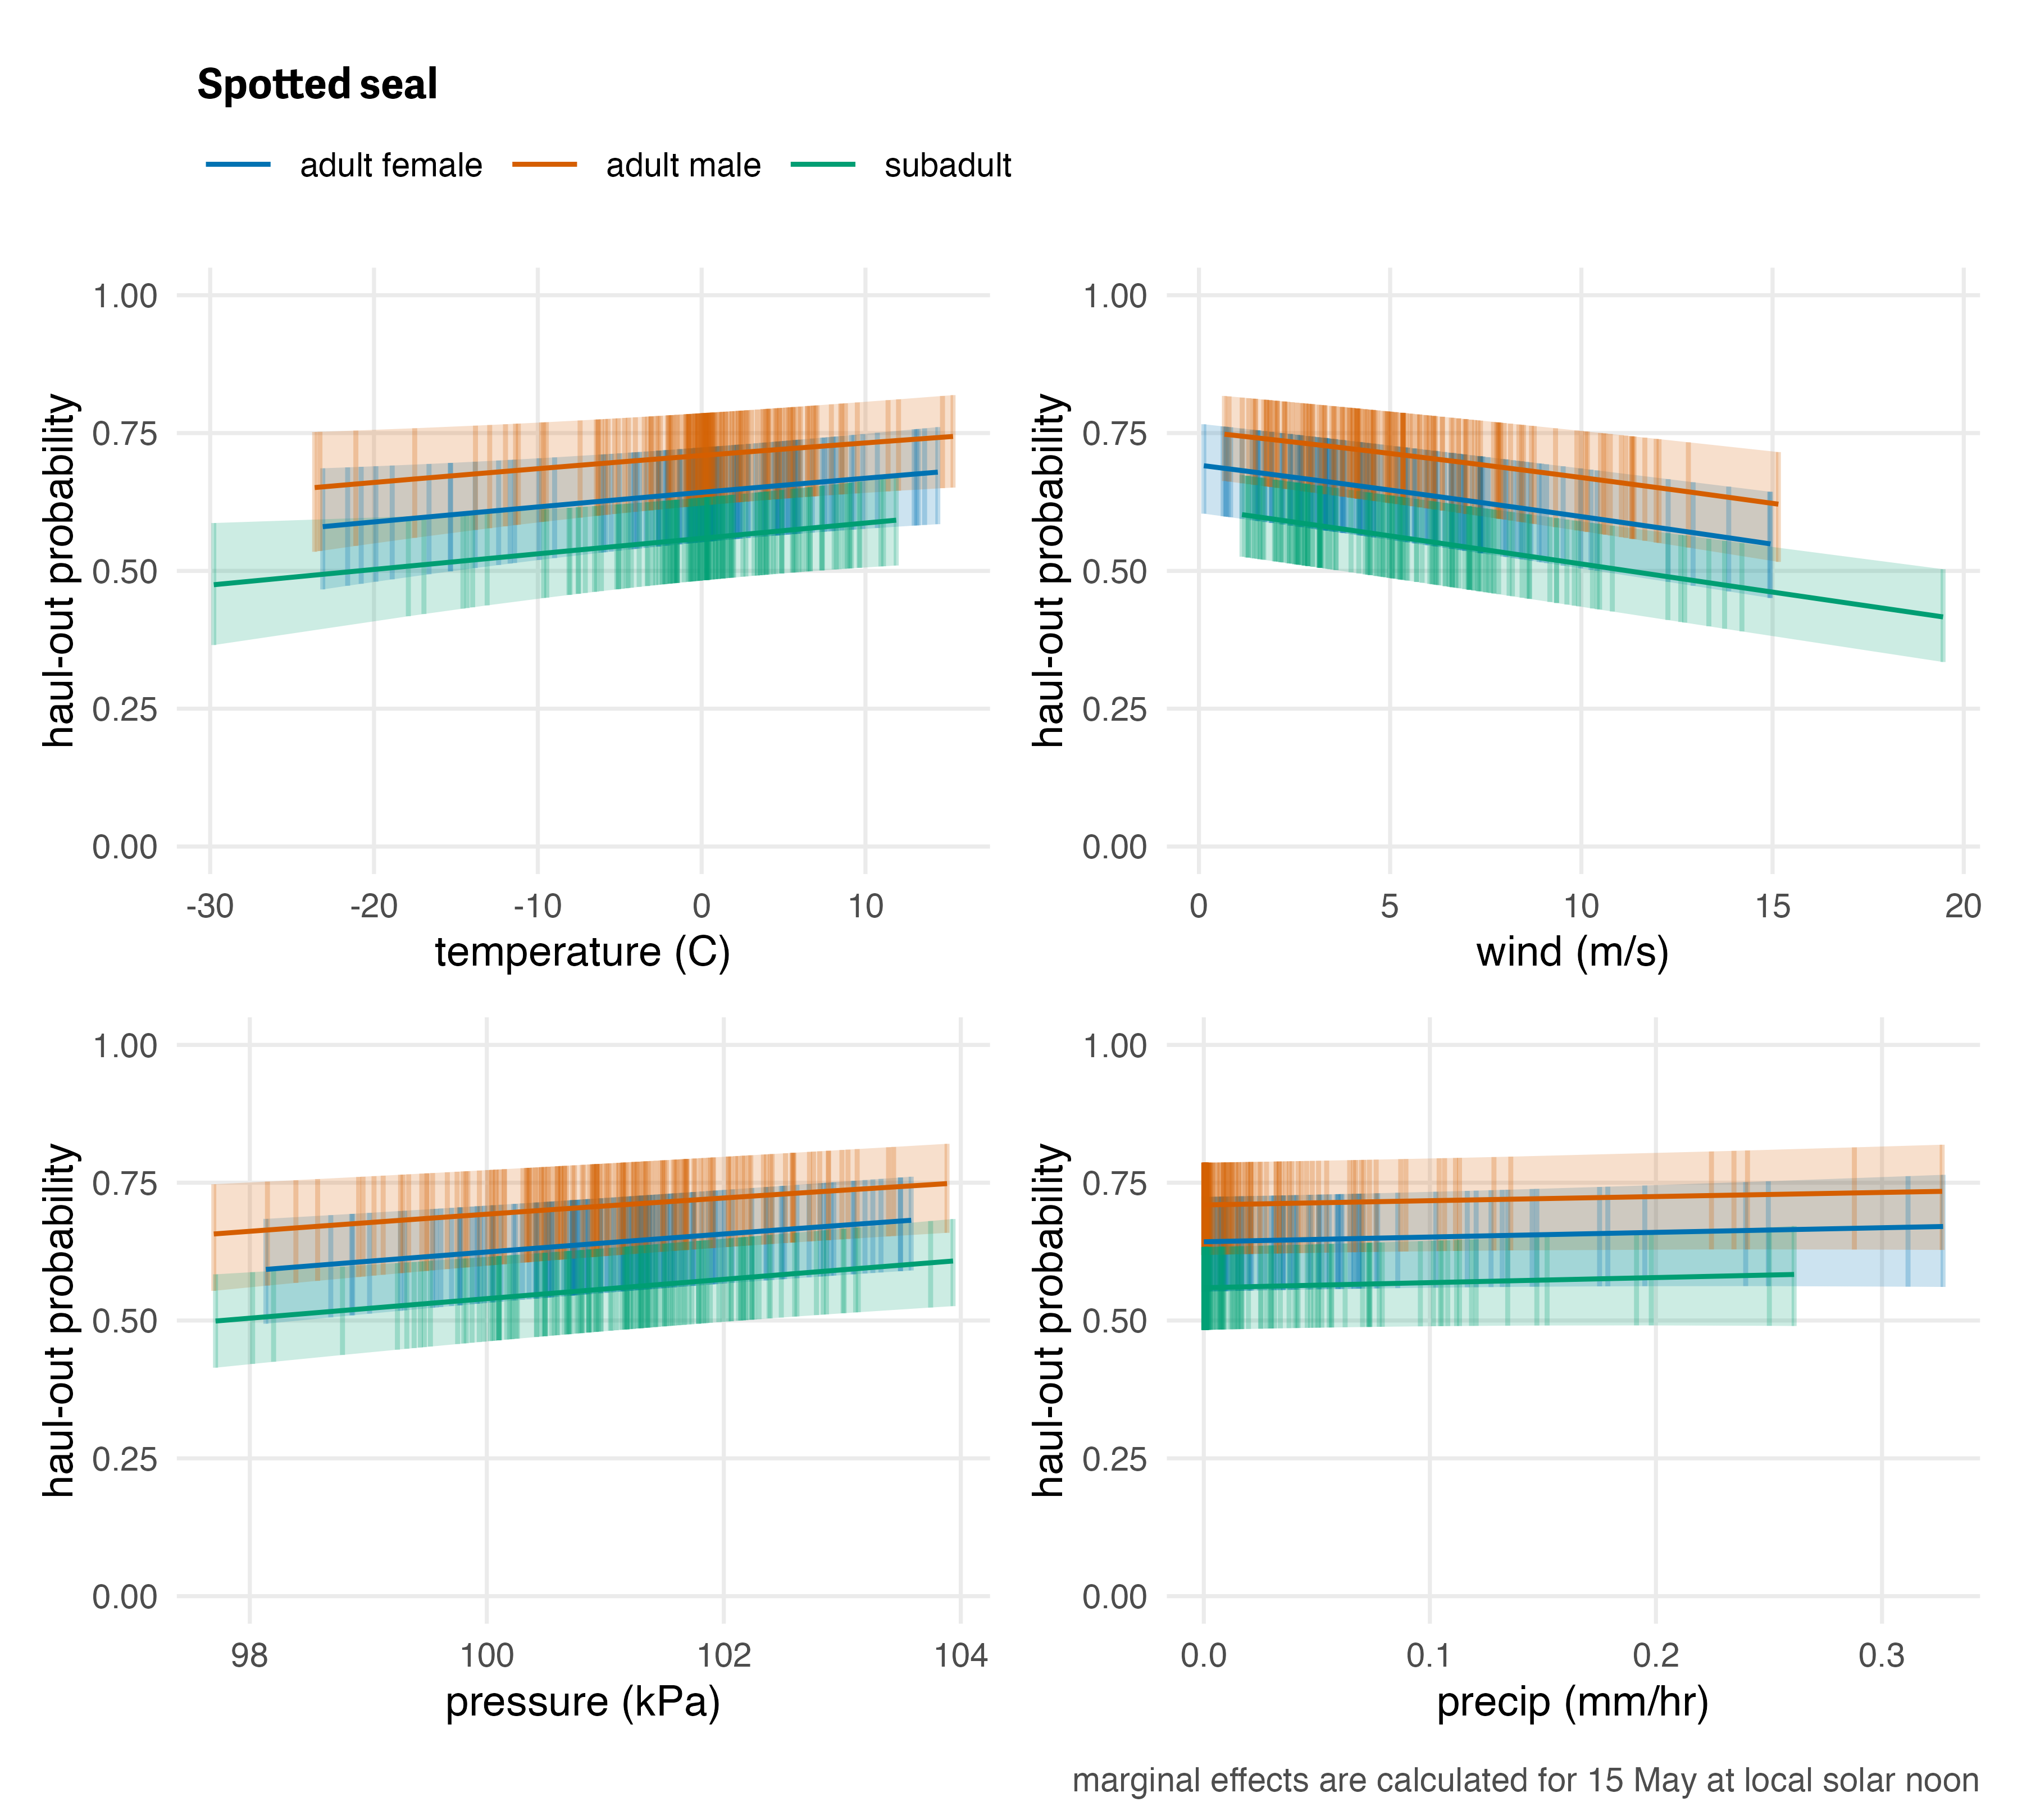
\includegraphics[width=1\linewidth]{../figures/Figure-010} \caption{\textbf{Influence of weather covariates on spotted seal haul-out probability} \linebreak Marginal effects of temperature, wind, barometric pressure, and precipitation on the predicted haul-out probability of spotted seals within each age and sex classification. Hour of the day was fixed at local solar noon and day-of-year fixed at 15 May. The other weather covariate values were predicted from a simple generalized additive model for each weather covariate with smooth terms for day-of-year and solar hour to account for anticipated variability within a day over the season. While the marginal effect of the covariate is continuous, points and vertical lines representing the 95\% confidence interval around the predicted haul-out probability are shown only at observed weather values to give an indication of how the observations are distributed across the range of weather values.}\label{fig:spottedHOwx}
\end{figure}

\subsection*{Annual variation in haul-out timing}\label{annual-variation-in-haul-out-timing}
\addcontentsline{toc}{subsection}{Annual variation in haul-out timing}

The second set of models, which included annual variation in haul-out
patterns, uncovered significant contributions for linear and quadratic
interactions between day and year for only spotted seals (\emph{day:year},
\(F_{15,115144}\)
= 4.445; \(p\) =
\textless0.001; \emph{day\textsuperscript{2}:year},
\(F_{15,115144}\)
= 5.854; \(p\) =
\textless0.001). Ribbon seals showed no significant
contribution for interactions between day and year (\emph{day:year},
\(F_{10,99510}\)
= 0.516; \(p\) =
0.880; \emph{day\textsuperscript{2}:year},
\(F_{10,99510}\)
= 0.549; \(p\) =
0.856). Predicted distributions of
haul-out activity were largely unimodal, but varied some among and
within years with respect to the timing and magnitude of haul-out peaks
(Figure \ref{fig:annualHO}). It is important to note that predicted
variation in annual haul-out patterns likely reflected both process error
and sampling variability. While we did remove any years where only one
deployment in a species + age:sex group was present, there were still
some years where the pattern shown was informed by a small number of
individuals that may not represent population-level patterns.



\begin{figure}
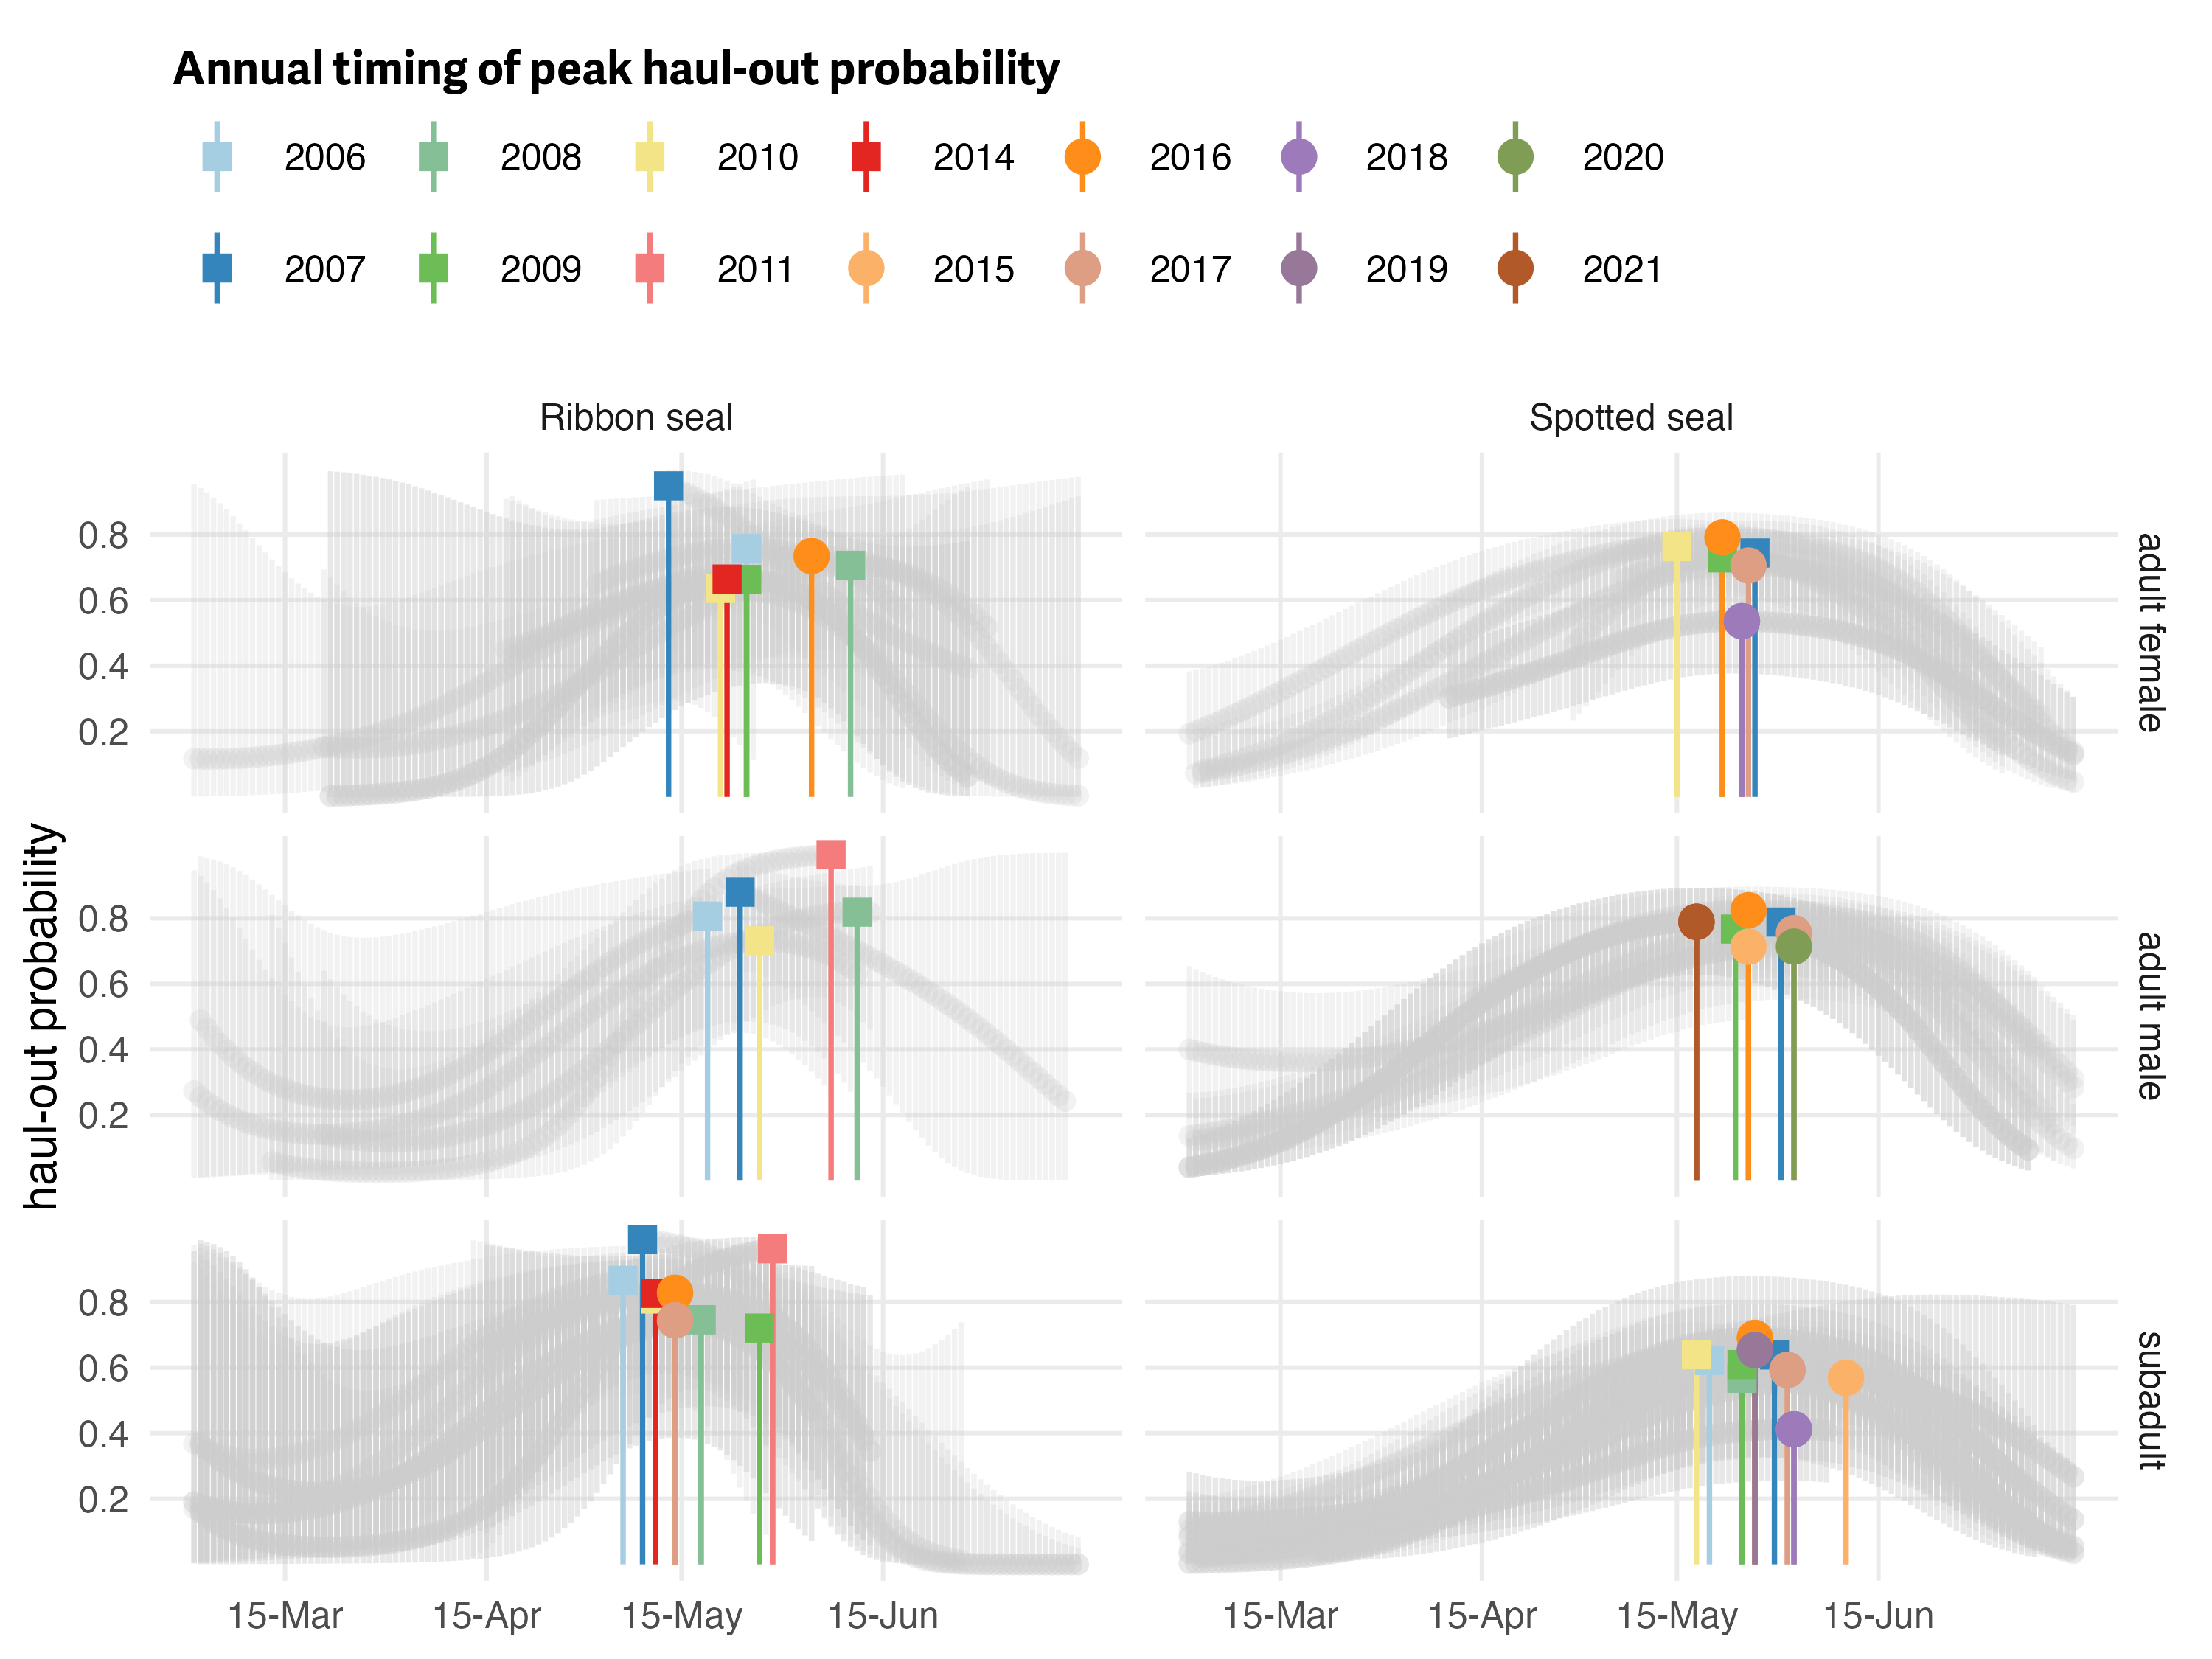
\includegraphics[width=1\linewidth]{../figures/Figure-011} \caption{\textbf{Annual variability in the timing of peak haul-out probability for ribbon and spotted seals.} \linebreak Spring haul-out probability (colored markers) for ribbon and spotted seals across 14 years are shown. The full seasonal range of annual predictions along with uncertainty are presented as grey lines. Covariates were fixed at local solar noon and weather covariate values were predicted from a simple generalized additive model for each weather covariate with smooth terms for day-of-year and solar hour to account for anticipated variability within a day over the season. Only those groups (age:sex + year) that included observations from more than one seal are shown. Additionally, any groups where data were only available after 1 June or before 1 May are not included.}\label{fig:annualHO}
\end{figure}

The annual timing of peak haul-out probability for ribbon seals and adult
male spotted seals appeared to have
no relationship with the amount of yearly maximum sea-ice extent in the
study area. For ribbon seals and adult male spotted seals,
\(p\)-values were substantially larger than 0.05 (ribbon seal adult
females; \(R^{2}\) = 0.004, \(p\) = 0.896;
ribbon seal adult males: \(R^{2}\) = 0.059, \(p\) =
0.693; ribbon seal subadults: \(R^{2}\) =
0.007, \(p\) = 0.828; spotted seals
adult males: \(R^{2}\) = 0.004, \(p\) =
0.889). Adult female and subadult spotted seals both
showed a negative trend (peak haul-out occurs later in years with less
sea ice) but neither with a significant relationship\\
(spotted seal adult female: \(R^{2}\) =
0.456, \(p\) = 0.141; spotted seal
subadults: \(R^{2}\) = 0.369, \(p\) =
0.062).

\section*{Discussion}\label{discussion}
\addcontentsline{toc}{section}{Discussion}

We modeled data from bio-loggers deployed on bearded, ribbon, and spotted seals
to examine factors affecting their haul-out behavior on sea ice in the Bering
and Chukchi seas. Our analysis shows all three species of seal haul out
progressively more through the spring and peak near mid-May to early June before
declining again. This pattern aligns well with what has been previously
documented qualitatively (Boveng et al., 2009; Cameron et al., 2010; Boveng \& Cameron, 2013) and confirms
our haul-out data are likely quantifying population-level behavioral patterns.
Beginning in spring, seals preferentially haul out on ice shortly after solar
noon, which allows seals to maximize absorption of solar radiation thought to
facilitate the molting process (Feltz \& Fay, 1966). Interestingly, bearded seals appear
to have two peaks in haul-out activity within a day, one shortly after solar
noon, and one centered near solar midnight. This, of course, could be an
artifact of our limited sample size for bearded seal deployments across all age
classes. However, a similar bi-modal pattern has been seen in ringed seals
(Von Duyke et al., 2020) and suggests that bearded and ringed seals may be operating
under different constraints than ribbon and spotted seals. Bearded and ringed
seals are distributed across higher latitudes that experience
extended daylight hours during spring which may allow more flexibility in
alternating resting and foraging events. Other factors such as predation by
polar bears (which is rare for ribbon and spotted seals in the Bering Sea) may
also explain differing haul-out patterns. The change in haul-out behavior during
the season was less pronounced in bearded seals compared to ribbon and spotted
seals. This aligns with findings from Thometz et al. (Thometz et al., 2021) who observed
a mean molting period of 119±2 days and a relatively stable resting metabolic
rate for bearded seals during that time. While ribbon seals were not considered
in that study, spotted and ringed seals underwent molt periods of just 33±4
and 28±6 days and had increased resting metabolic rates.

Unlike previous analyses of seal haul-out behavior in spotted and ribbon seals
(e.g. (Ver Hoef, London \& Boveng, 2010), (Conn et al., 2014)), we also investigated the influence of
sex-age class on haul-out probabilities of both species (but not for bearded seals
because of low sample size). Field identification of age class can be inexact,
particularly when differentiating subadults from adults. In the case of ribbon
seals, subadults often have less distinct ribbons than adults. Spotted seal
pelage cannot be used to reliably discern adults from subadults. Despite these
challenges, we feel the age classifications used in this analysis are useful in
testing for age-related effects on haul-out behavior.

Although ribbon and spotted seals exhibited a
unimodal diel haul-out pattern generally centered around local solar noon, there
were key differences across species, age, and sex that match our understanding
from natural history descriptions of their ecological behavior. Spotted seals
are known to form triads during the breeding season where a female and dependent
pup are accompanied on the ice by a suitor male (Frost \& Burns, 2018). The male waits for
the female to wean the pup and enter estrus, and fends off any other potential
suitor males. Triad formation results in both males and females spending a large
portion of the day hauled out on ice and a protracted spring haul-out season for
both sexes. While females are still nursing the pup and not yet in estrus they
may be less inclined to interrupt their haul out and enter the water where the
suitor male would attempt mating. We see this reflected in the predicted
haul-out patterns, with both males and females exhibiting a broad distribution
of time out of the water throughout the solar day and the season. Ribbon seals
are not known to form triads and our model predicts a progression of increased
haul-out behavior with females starting earlier in the season than males.
Notably, female ribbon seals spend a large portion of the day in the water
during the pupping period, aligning with the hypothesis that ribbon seal females
continue foraging while nursing. Subadult ribbon and spotted seals begin
elevated haul-out behavior earlier in the spring and follow a pattern seen in
other phocids where yearlings and subadults molt first followed by adult females
and males (Thompson \& Rothery, 1987; Kirkman et al., 2003; Reder et al., 2003). Also of note is the early
development in newly weaned pups of haul-out behavior centered around solar noon
observed in this study.

We also investigated the influence of weather on haul-out probabilities,
including wind speed, temperature, barometric pressure, precipitation, and wind
chill. These have been investigated for walruses (e.g.~Udevitz et al.
(2009)) and a few select studies of ice-associated seals
(Perry, Stenson \& Buren, 2017; Hamilton \& Evans, 2018). In our study, ribbon seal haul-out behavior was notably
influenced by weather, with wind, temperature, and barometric pressure all being
important components of the model. Spotted seals were most affected by wind and
barometric pressure. For bearded seals, the model indicated wind and temperature
had the greatest impact. In general, and as might be expected, seals were more
likely to haul-out when daily temperatures were warmer, winds speeds were lower,
barometric pressure was higher, and precipitation was lower. Those weather
conditions are general indicators of increased solar radiation and lower
convective heat loss, both of which provide energetic benefits (see additional
discussion in Supplemental Material \hyperref[exploring-insolation-solar-radiation-as-a-model-covariate]{Exploring Insolation (Solar Radiation) as a
Model Covariate} regarding the potential use of solar radiation directly). Low
winds and precipitation could also enhance predator detection. Our results
highlight the importance of incorporating weather covariates when analyzing
haul-out behavior and calculating availability corrections for aerial surveys.

Notably missing from our list of haul-out model explanatory variables is any
spatial-temporal representation of sea-ice concentration, area, or extent. This
may seem counterintuitive when modeling the haul-out behavior of seal species
with such a close association to sea ice; seals haul out in the presence of sea
ice, and we could assess the local concentration of sea ice during these events
(see (Olnes et al., 2020)). This, however, expands the scope of our analysis into the
realm of habitat selection and many of our deployments consisted of a single
device attached to the rear flipper of the seal which meant we only received
locations when seals were hauled out on sea ice, limiting our ability to fully
evaluate fine-scale habitat preferences related to sea ice. Insight into how
seals use and interact with sea ice during an extended period when the
availability and characteristics of sea ice is rapidly changing is important
(Breed et al., 2018; Cameron et al., 2018) but ancillary to the focus of this analysis -- and,
in the end, not possible given key limitations of our data. Additionally, our
study was limited to the spring season when seal haul-out behaviors are strongly
influenced by pupping, nursing, breeding behavior, and molt. These drivers are
likely more influential on haul-out behavior than sea-ice concentration.
Crawford et al. (2019) compared haul-out probability models for ringed
seals and found those that only included season (and not sea-ice concentration)
were the most parsimonious. For all of these reasons, we have elected not to use
sea-ice concentration \emph{as a predictor for haul-out probability} in the present
study.

Our models detected small deviations in the timing and magnitude of annual peaks
in haul-out behavior for ribbon and spotted seals. The timing of peak haul-out
activity appears to fall within a relatively narrow time window of 3-4 weeks in
late May and early June. This consistency across 15 years is likely a reflection
of the relationship between a critical photoperiod and the timing of important
life history stages (Temte, 1994; Bronson, 2009). However, along with a critical
photoperiod, ribbon and spotted seals are dependent upon the presence of sea ice
for pupping and molt. We did not find large support in our models for a
relationship between the timing of peaks in haul-out behavior and the amount of
yearly maximum sea ice. This could indicate that, while the extent of spring sea
ice in the Bering Sea varied widely during our study period, seals were still
able to locate sea ice and haul out. Only a small portion of our data was from
2018 -- 2019, years of extreme low spring ice extent in the Bering Sea that
appeared to impact body condition of ribbon and spotted seals (Boveng et al., 2020), so
we may currently lack sufficient contrast in ice extent to characterize an
effect on the timing of peak haul-out probability. We should expect, however,
that some minimal threshold in the spatial extent or density of sea ice will
have a meaningful impact on the timing of peak haul-out behavior --- if there is
no sea-ice, seals will not haul out or they will be forced to use terrestrial
haul-out sites which were not part of the evolution of their normal behaviors.
Additionally, while from an ecological perspective the haul-out behavior appears
consistent, the interannual differences in timing and magnitude are large enough
to have important ramifications on calculations of abundance and trend. Those
ramifications will only be exacerbated if climate variability amplifies
interannual differences.

Previous attempts to estimate the abundance of phocid seals from aerial survey
data in the Bering and Chukchi seas (e.g. Bengtson et al. (2005), Conn et al. (2014),
Ver Hoef et al. (2014)) have used estimated haul-out probabilities to correct for the
proportion of animals that are in the water and thus unavailable to be counted.
Although several of these studies allowed haul-out probabilities to vary by
day-of-year and time-of-day, they have not accounted for variability among
years, weather conditions, or in the age-sex class of the sample. In this paper,
we have shown that there can be considerable differences in the haul-out
probability of seals on ice based on these factors and subsequent analyses have
shown the potential for considerable bias in abundance estimates if such
covariates are unaccounted for (see Conn \& Trukhanova (2023) for discussion about the
importance of including stable age- and stage-proportions). We recommend that
future abundance analyses employ availability models that account for them. For
instance, it is relatively straightforward to obtain weather reanalysis products
(e.g.~NARR, ERA5) for times and locations that are surveyed and to construct a
relevant correction factor based on predictions of GLMPMs. The most challenging
element in developing availability correction factors is with annual
variability. It can be difficult to get a sufficient sample size to estimate
year-specific correction factors, particularly because research teams would
likely need to deploy bio-loggers on seals and conduct aerial surveys
concurrently, requiring considerably more personnel and money. One possible
suggestion is to include year as a random effect within models for aerial survey
counts such that, without specific knowledge of any particular year, the
among-year variance is included in the modeled standard errors. Regardless of
the specific approach, future estimates of Arctic seal abundance will require
specific consideration of annual variability and changes in the timing of peak
haul-out behavior when estimating trends, as one will not know if moderate
differences in abundance estimates are attributable to changes in abundance or
changes in haul-out behavior.

Predictions of absolute haul-out probability in this paper were somewhat
different than those previously reported for these species, especially for
bearded seals. For instance, Ver Hoef et al. (2014) and Conn et al.
(2014) used haul-out correction factors with maximums of 0.66 for bearded
seals, 0.62 for ribbon seals, and 0.54 for spotted seals, where these maximums
corresponded to times near local solar noon in mid-late May. Results here
suggest a haul-out probability on May 20 at local solar noon of 0.304
(95\% CI: 0.258 -- 0.354)
for bearded seals across all age and sex classes,
0.715
(95\% CI: 0.62 -- 0.794) for
adult male ribbon seals, 0.661
(95\% CI: 0.576 -- 0.738) for
adult female ribbon seals, 0.74
(95\% CI: 0.654 -- 0.811) for
adult male spotted seals, and 0.66
(95\% CI: 0.571 -- 0.739) for
adult female spotted seals. Our estimates
of haul-out probability reflect increased sample sizes in terms of
number of individuals, inclusion of weather covariates, and improvements to the
way data were prepared prior to analysis and should be the basis for any
future estimates of seal abundance from aerial surveys in the Bering and
Chukchi seas.

We focused this paper on haul-out behavior of bearded, ribbon, and spotted
seals. Ringed seals are also present in the Bering and Chukchi seas but exhibit
a unique complicating factor. Adult ringed seals build subnivean lairs under the
snow on top of the sea ice, where they haul out and where females rear pups
until conditions are good for basking (Frost et al., 2004). Thus, the wet-dry sensor on
a bio-logger could indicate that an animal is hauled out, but if it is within a
lair, it is not available to be detected during an aerial survey. We hope to
address availability of ringed seals using data from satellite tags, replicate
survey tracks, and auxiliary information about snow depth and timing of melt in
a future study (see, e.g., Lindsay et al. (2021)).

Our analysis emphasizes the importance of accounting for seasonal and temporal
variation in haul-out behavior, as well as associated weather covariates,
when interpreting the number of seals counted in aerial surveys. The rapid
acceleration of climate change in Arctic ecosystems is already occurring and is
forecast to decrease the quantity and quality of suitable habitat for
ice-associated seals that rely on sea-ice for a variety of activities. Improved
estimates of seal population abundance from aerial surveys are needed to
properly monitor the impacts of these changes on seal populations over time.
Those monitoring surveys will need to be paired with continued investigation and
assessment of seal haul-out behavior to allow credible predictions about the
effects of climate disruptions on the abundance and distribution of Arctic seal
populations.

\section*{Author Contributions}\label{author-contributions}
\addcontentsline{toc}{section}{Author Contributions}

\begin{itemize}
\tightlist
\item
  \textbf{Josh M. London}: investigation, conceptualization, methodology,
  formal analysis, validation, software, writing: original draft, writing:
  review and editing, visualization, and data curation
\item
  \textbf{Paul B. Conn}: conceptualization, methodology, formal analysis,
  software, validation, writing: original draft, writing: review and
  editing
\item
  \textbf{Stacie K. Hardy}: investigation, data curation, methodology,
  validation, writing: review and editing
\item
  \textbf{Erin L. Richmond}: data curation, investigation, methodology,
  validation, writing: review and editing
\item
  \textbf{Jay M. Ver Hoef}: conceptualization, methodology, software, writing:
  review and editing
\item
  \textbf{Michael F. Cameron}: investigation, project administration, writing:
  review and editing
\item
  \textbf{Justin A. Crawford}: investigation, methodology, validation, data curation,
  writing: review and editing
\item
  \textbf{Lori T. Quakenbush}: investigation, methodology, supervision, project
  administration, writing: review and editing
\item
  \textbf{Andrew L. Von Duyke}: investigation, methodology, validation, data curation,
  writing: review and editing
\item
  \textbf{Peter L. Boveng}: investigation, conceptualization, supervision,
  project administration, writing: review and editing
\end{itemize}

\section*{Data Availability}\label{data-availability}
\addcontentsline{toc}{section}{Data Availability}

This manuscript was developed as a reproducible research compendium and was
originally published as a pre-print at bioRxiv (London et al. (2022);
\url{https://doi.org/10.1101/2022.04.07.487572}). All data used in the study and code
are available on GitHub (\url{https://github.com/noaa-afsc/berchukseals-haulout}) and
major versions archived at Zenodo (\url{https://doi.org/10.5281/zenodo.4638221}).
Original data sources for telemetry are archived as part of datasets at
the United States Animal Telemetry Network (\url{https://portal.atn.ioos.us/};
\url{https://doi.org/10.24431/rw1k8er}), archived at Movebank (see
Movebank ID 732321226), or associated
with other published manuscripts (see supplemental material
\ref{tab:deploymentTable}). Collated and cleaned data products needed to
replicate the analysis along with the results of all model fits are also
available and versioned as an R package on GitHub
(\url{https://github.com/noaa-afsc/berchuksealsHauloutFits}) and archived at Zenodo
(\url{https://doi.org/10.5281/zenodo.10056308}).

\section*{Acknowledgments}\label{acknowledgments}
\addcontentsline{toc}{section}{Acknowledgments}

We recognize that the species and ecosystems we studied are within the ancestral
and present-day environs of the Inupiat and Yup'ik people who, through many
uncredited contributions of traditional knowledge, provided early western
naturalists and scientists with much of what gets described as the `basic
biology' of Arctic seals. The deployment of bio-logging devices used in this
study were often done in collaboration with Alaska Native seal hunters and wiht the
approval of
their communities. We would like to especially acknowledge the Alaska communities of
Kotzebue, Koyuk, Nome, Nuiqsut, Scammon Bay, St.~Michael, Utqiaġvik, and Ulguniq
(Wainwright) and the following individuals: James Adams, Jeff Barger, David
Barr, Wendell Booth, Cyrus Harris, Nereus `Doc' Harris, Grover Harris, Lee
Harris, Tom Jones, Frank Garfield, Brenda Goodwin, Henry Goodwin, John Goodwin,
Pearl Goodwin, Willie Goodwin, Brett Kirk, Noah Naylor, Virgil Naylor Jr.,
Virgil Naylor Sr., Dan Savetilik, Chuck Schaeffer, Ross Schaeffer, Allen Stone,
and Randy Toshavik from Kotzebue; Merlin Henry from Koyuk; Tom
Gray from Nome; Vernon Long and Richard Tukle from Nuiqsuit; Morgan
Simon, River Simon, and Al Smith from Scammon Bay; Alex Niksik Jr.~from
St.~Michael; Billy Adams, James Aiken, Tim Aiken, Howard Kittick,
Gilbert Leavitt, Isaac Leavitt, J.R. Leavitt, Bobby Sarren, and Joe Skin from Utqiaġvik;
Mary Ellen Ahmaogak, Enoch Oktollik, Shawn Oktollik, Stacey Osborn, and
Fred Rexford from Ulguniq. We would also like to acknowledge the support of the
Ice Seal Committee.

We are grateful for the assistance in catching and sampling seals by Ryan Adam,
James Bailey, Michelle Barbieri, John Bengtson, Gavin Brady, Anna Bryan,
Vladamir Burkanov, Cynthia Christman, Sarah Coburn, Shawn Dahle, Rob Delong,
Stacy DiRocco, Deb Fauquier, Shannon Fitzgerald, Kathy Frost, Scott Gende, Craig
George, Tracey Goldstein, Jeff Harris, Jason Herreman, Markus Horning, John
Jansen, Shawn Johnson, Charles Littnan, Lloyd Lowry, Brett McClintock, Erin
Moreland, Aaron Morris, Mark Nelson, Justin Olnes, Lorrie Rea, Bob Shears, Gay
Sheffield, Kayla Scheimreif, Brent Stewart, Alexy Trukhin, Dave Withrow, and
Heather Ziel. We also appreciate the commitment to science and safety by all
officers and crew of the NOAA ship \emph{Oscar Dyson}, the NOAA ship \emph{MacArthur II},
the \emph{MV Tayfun}, and the RV \emph{Thomas G. Thompson}.

Telemetry data from the Alaska Department of Fish and Game (ADF\&G) and the North
Slope Borough Department of Wildlife Management (NSB) were important
contributions to the findings presented here. Deployments in the western Bering
Sea were done in collaboration with Russian colleagues and North Pacific
Wildlife Consulting, LLC.

The findings and conclusions in the paper are those of the author(s) and do not
necessarily represent the views of the National Marine Fisheries Service, NOAA.
Any use of trade, product, or firm names does not imply an endorsement by the
U.S. Government.

\section*{References}\label{references}
\addcontentsline{toc}{section}{References}

\phantomsection\label{refs}
\begin{CSLReferences}{1}{0}
\bibitem[\citeproctext]{ref-bengtson2004}
Bengtson JL, Cameron MF. 2004. Seasonal haulout patterns of crabeater seals (\emph{Lobodon carcinophaga}). \emph{Polar Biology} 27:344--349. DOI: \href{https://doi.org/DOI\%2010.1007/s00300-004-0597-1}{DOI 10.1007/s00300-004-0597-1}.

\bibitem[\citeproctext]{ref-bengtson2005a}
Bengtson JL, Hiruki-Raring LM, Simpkins MA, Boveng PL. 2005. Ringed and bearded seal densities in the eastern Chukchi Sea, 1999-2000. \emph{Polar Biology} 28:833--845.

\bibitem[\citeproctext]{ref-betts2006}
Betts MG, Diamond A, Forbes G, Villard M-A, Gunn J. 2006. The importance of spatial autocorrelation, extent and resolution in predicting forest bird occurrence. \emph{Ecological Modelling} 191:197--224.

\bibitem[\citeproctext]{ref-boveng2009}
Boveng PL, Bengtson JL, Buckley TW, Cameron MF, Dahle SP, Kelly BP, Megrey BA, Overland JE, Williamson NJ. 2009. \href{https://repository.library.noaa.gov/view/noaa/3671}{Status review of the spotted seal (\emph{Phoca largha})}. \emph{U.S. Dep. Commer., NOAA Tech. Memo.} NMFS-AFSC-200:153.

\bibitem[\citeproctext]{ref-boveng2013a}
Boveng PL, Bengtson JL, Cameron MF, Dahle SP, Logerwell EA(ElizabethA), London JM, Overland JE, Sterling JT, Stevenson DE 1970-, Taylor BL 1954-, Ziel HL 1974-. 2013. \href{https://repository.library.noaa.gov/view/noaa/4451}{Status review of the ribbon seal (\emph{Histriophoca fasciata})}. \emph{U.S. Dep. Commer., NOAA Tech. Memo.} NMFS-AFSC-255:174.

\bibitem[\citeproctext]{ref-boveng2013}
Boveng PL, Cameron MF. 2013. \emph{Pinniped movements and foraging: seasonal movements, habitat selection, foraging and haul-out behavior of adult bearded seals in the Chukchi Sea. Final Report, BOEM Report 2013-01150}. Anchorage, Alaska: Bureau of Ocean Energy Management, Alaska Outer Continental Shelf Region.

\bibitem[\citeproctext]{ref-boveng2018a}
Boveng P, Lowry L. 2018. Ribbon seal (\emph{Histriophoca fasciata}). In: Bernd Würsig, J. G. M. Thewissen, Kit Kovacs eds. \emph{Encyclopedia of Marine Mammals: Third Edition}. London: Academic Press, 811--813.

\bibitem[\citeproctext]{ref-boveng2020}
Boveng PL, Ziel HL, McClintock BT, Cameron MF. 2020. Body condition of phocid seals during a period of rapid environmental change in the Bering Sea and Aleutian Islands, Alaska. \emph{Deep Sea Research Part II: Topical Studies in Oceanography} 181-182:104904. DOI: \href{https://doi.org/10.1016/j.dsr2.2020.104904}{10.1016/j.dsr2.2020.104904}.

\bibitem[\citeproctext]{ref-breed2018}
Breed GA, Cameron MF, Ver Hoef JM, Boveng PL, Whiting A, Frost KJ. 2018. Seasonal sea ice dynamics drive movement and migration of juvenile bearded seals \emph{Erignathus barbatus}. \emph{Marine Ecology Progress Series} 600:223--237.

\bibitem[\citeproctext]{ref-bronson2009}
Bronson FH. 2009. Climate change and seasonal reproduction in mammals. \emph{Philosophical Transactions of the Royal Society B} 364:3331--3340. DOI: \href{https://doi.org/10.1098/rstb.2009.0140}{10.1098/rstb.2009.0140}.

\bibitem[\citeproctext]{ref-cameron2010}
Cameron MF, Bengtson JL, Boveng PL, Jansen JK(JohnK, Kelly BP, Dahle SP, Logerwell EA(ElizabethA), Overland JE, Sabine CL, Waring GT, Wilder JM. 2010. \href{https://repository.library.noaa.gov/view/noaa/3761}{Status review of the bearded seal (\emph{Erignathus barbatus})}. \emph{U.S. Dep. Commer., NOAA Tech. Memo.} NMFS-AFSC-211:246.

\bibitem[\citeproctext]{ref-cameron2018}
Cameron MF, Frost KJ, Ver Hoef JM, Breed GA, Whiting AV, Goodwin J, Boveng PL. 2018. Habitat selection and seasonal movements of young bearded seals (\emph{Erignathus barbatus}) in the Bering Sea. \emph{PLoS ONE} 13:e0192743. DOI: \href{https://doi.org/10.1371/journal.pone.0192743}{10.1371/journal.pone.0192743}.

\bibitem[\citeproctext]{ref-cavalieri1996}
Cavalieri DJ, Parkinson CL, Gloersen P, Zwally H. 1996.Sea ice concentrations from Nimbus-7 SMMR and DMSP SSM/I-SSMIS passive microwave data. Boulder, Colorado USA: NASA National Snow and Ice Data Center Distributed Active Archive Center

\bibitem[\citeproctext]{ref-conn2014a}
Conn PB, Hoef JMV, McClintock BT, Moreland EE, London JM, Cameron MF, Dahle SP, Boveng PL. 2014. \href{https://onlinelibrary.wiley.com/doi/abs/10.1111/2041-210X.12127}{Estimating multispecies abundance using automated detection systems: Ice-associated seals in the Bering Sea}. \emph{Methods in Ecology and Evolution} 5:1280--1293.

\bibitem[\citeproctext]{ref-conn2012c}
Conn PB, Johnson DS, London JM, Boveng PL. 2012. Accounting for missing data when assessing availability in animal population surveys: an application to ice-associated seals in the Bering Sea. \emph{Methods in Ecology and Evolution}:1039--1046.

\bibitem[\citeproctext]{ref-conn2023}
Conn PB, Trukhanova IS. 2023. Modeling vital rates and age-sex structure of Pacific Arctic phocids: influence on aerial survey correction factors. \emph{Marine Mammal Science} 39:648--661. DOI: \href{https://doi.org/10.1111/mms.12992}{10.1111/mms.12992}.

\bibitem[\citeproctext]{ref-crawford2019}
Crawford JA, Frost KJ, Quakenbush LT, Whiting A. 2019. Seasonal and diel differences in dive and haul-out behavior of adult and subadult ringed seals (\emph{Pusa hispida}) in the Bering and Chukchi seas. \emph{Polar Biology} 42:65--80. DOI: \href{https://doi.org/10.1007/s00300-018-2399-x}{10.1007/s00300-018-2399-x}.

\bibitem[\citeproctext]{ref-crawford2015}
Crawford JA, Quakenbush LT, Citta JJ. 2015. A comparison of ringed and bearded seal diet, condition and productivity between historical (1975-1984) and recent (2003-2012) periods in the Alaskan Bering and Chukchi seas. \emph{Progress in Oceanography} 136:133--150. DOI: \href{https://doi.org/10.1016/j.pocean.2015.05.011}{10.1016/j.pocean.2015.05.011}.

\bibitem[\citeproctext]{ref-feltz1966}
Feltz ET, Fay FH. 1966. Thermal requirements in vitro of epidermal cells from seals. \emph{Cryobiology} 3:261--264.

\bibitem[\citeproctext]{ref-frost2018}
Frost KJ, Burns JJ. 2018. Spotted Seal: \emph{Phoca largha}. In: Würsig B, Thewissen JGM, Kovacs KM eds. \emph{Encyclopedia of Marine Mammals (Third Edition)}. Academic Press, 928--931. DOI: \href{https://doi.org/10.1016/B978-0-12-804327-1.00244-2}{10.1016/B978-0-12-804327-1.00244-2}.

\bibitem[\citeproctext]{ref-frost2004}
Frost KJ, Lowry LF, Pendleton G, Nute HR. 2004. Factors affecting the observed densities of ringed seals, \emph{Phoca hispida}, in the Alaskan Beaufort Sea, 1996-99. \emph{Arctic} 57:115--128.

\bibitem[\citeproctext]{ref-hamilton2018}
Hamilton V, Evans K. 2018. Establishing growth chronologies from marine mammal teeth: a method applicable across species. \emph{Journal of Experimental Marine Biology and Ecology} 505:24--34. DOI: \url{https://doi.org/10.1016/j.jembe.2018.04.006}.

\bibitem[\citeproctext]{ref-harwood2020}
Harwood LA, Smith TG, Alikamik J, Alikamik E, Lea EV, Stirling I, Wright H, Melling H, Zhu X. 2020. Long-term, harvest-based monitoring of ringed seal body condition and reproduction in Canada's western arctic: an update through 2019. \emph{Arctic} 73:206--220. DOI: \href{https://doi.org/10.14430/arctic70428}{10.14430/arctic70428}.

\bibitem[\citeproctext]{ref-huntington2020}
Huntington HP, Danielson SL, Wiese FK, Baker M, Boveng P, Citta JJ, De Robertis A, Dickson DMS, Farley E, George JC, Iken K, Kimmel DG, Kuletz K, Ladd C, Levine R, Quakenbush L, Stabeno P, Stafford KM, Stockwell D, Wilson C. 2020. Evidence suggests potential transformation of the Pacific Arctic ecosystem is underway. \emph{Nature Climate Change}:342--348. DOI: \href{https://doi.org/10.1038/s41558-020-0695-2}{10.1038/s41558-020-0695-2}.

\bibitem[\citeproctext]{ref-johnson2008a}
Johnson DS, London JM, Lea M-A, Durban JW. 2008. Continuous-time correlated random walk model for animal telemetry data. \emph{Ecology} 89:1208--1215.

\bibitem[\citeproctext]{ref-kelly2010}
Kelly BP, Bengtson JL, Boveng PL, Cameron MF, Dahle SP, Jansen JK, Logerwell EA, Overland JE, Sabine CL, Waring GT, Wilder JM. 2010. \emph{\href{https://repository.library.noaa.gov/view/noaa/3762}{Status review of the ringed seal (\emph{Phoca hispida})}}. U.S. Department of Commerce.

\bibitem[\citeproctext]{ref-kelly1990c}
Kelly BP, Quakenbush LT. 1990. Spatiotemporal use of lairs by ringed seals (\emph{Phoca hispida}). \emph{Canadian Journal of Zoology} 68:2503--2512.

\bibitem[\citeproctext]{ref-kirkman2003}
Kirkman SP, Bester MN, Pistorius PA, Hofmeyr GJG, Jonker FC, Owen R, Strydom N. 2003. Variation in the timing of moult in southern elephant seals at Marion Island : research article. \emph{South African Journal of Wildlife Research - 24-month delayed open access} 33:79--84. DOI: \href{https://doi.org/10.10520/EJC117173}{10.10520/EJC117173}.

\bibitem[\citeproctext]{ref-kwok2018}
Kwok R. 2018. Arctic sea ice thickness, volume, and multiyear ice coverage: losses and coupled variability (1958--2018). \emph{Environmental Research Letters} 13:105005. DOI: \href{https://doi.org/10.1088/1748-9326/aae3ec}{10.1088/1748-9326/aae3ec}.

\bibitem[\citeproctext]{ref-lindsay2021}
Lindsay JM, Laidre KL, Conn PB, Moreland EE, Boveng PL. 2021. \href{https://www.int-res.com/abstracts/esr/v46/p1-17/}{Modeling ringed seal \emph{Pusa hispida} habitat and lair emergence timing in the eastern Bering and Chukchi Seas}. \emph{Endangered Species Research} 46:1--17.

\bibitem[\citeproctext]{ref-london2022}
London JM, Conn PB, Hardy SK, Richmond EL, Ver Hoef JM, Cameron MF, Crawford JA, Von Duyke AL, Quakenbush LT, Boveng PL. 2022. Spring haul-out behavior of seals in the Bering and Chukchi seas. \emph{bioRxiv}:2022--04. DOI: \url{https://doi.org/10.1101/2022.04.07.487572}.

\bibitem[\citeproctext]{ref-london2012}
London JM, Ver Hoef JM, Jeffries SJ, Lance MM, Boveng PL. 2012. Haul-out behavior of harbor seals (\emph{Phoca vitulina}) in Hood Canal, Washington. \emph{PLoS ONE} 7:e38180. DOI: \href{https://doi.org/10.1371/journal.pone.0038180}{10.1371/journal.pone.0038180}.

\bibitem[\citeproctext]{ref-lonergan2013}
Lonergan M, Duck C, Moss S, Morris C, Thompson D. 2013. Rescaling of aerial survey data with information from small numbers of telemetry tags to estimate the size of a declining harbour seal population. \emph{Aquatic Conservation-Marine and Freshwater Ecosystems} 23:135--144. DOI: \href{https://doi.org/Doi\%2010.1002/Aqc.2277}{Doi 10.1002/Aqc.2277}.

\bibitem[\citeproctext]{ref-lopez2013}
Lopez R, Malardé JP, Royer F, Gaspar P. 2013. Improving Argos Doppler location using multiple-model Kalman filtering. \emph{Geoscience and Remote Sensing, IEEE Transactions on} PP:1--12. DOI: \href{https://doi.org/10.1109/tgrs.2013.2284293}{10.1109/tgrs.2013.2284293}.

\bibitem[\citeproctext]{ref-mclaren1958a}
McLaren IA. 1958. Some aspects of growth and reproduction of the bearded seal, \emph{Erignathus barbartus} (Erxleben). \emph{Journal of the Fisheries Research Board of Canada} 15:219--227.

\bibitem[\citeproctext]{ref-meier2014}
Meier WN, Hovelsrud GK, Oort BEH van, Key JR, Kovacs KM, Michel C, Haas C, Granskog MA, Gerland S, Perovich DK, Makshtas A, Reist JD. 2014. \href{https://agupubs.onlinelibrary.wiley.com/doi/abs/10.1002/2013RG000431}{Arctic sea ice in transformation: A review of recent observed changes and impacts on biology and human activity}. \emph{Reviews of Geophysics} 52:185--217.

\bibitem[\citeproctext]{ref-mesinger2006a}
Mesinger F, DiMego G, Kalnay E, Mitchell K, Shafran PC, Ebisuzaki W, Jović D, Woollen J, Rogers E, Berbery EH, Ek MB, Fan Y, Grumbine R, Higgins W, Li H, Lin Y, Manikin G, Parrish D, Shi W. 2006. North American Regional Reanalysis. \emph{Bulletin of the American Meteorological Society} 87:343--360. DOI: \href{https://doi.org/10.1175/BAMS-87-3-343}{10.1175/BAMS-87-3-343}.

\bibitem[\citeproctext]{ref-niemi2023}
Niemi M, Nykänen M, Biard V, Kunnasranta M. 2023. Seasonal changes in diel haul-out patterns of a lacustrine ringed seal (\emph{Pusa hispida saimensis}). \emph{Ecology and Evolution} 13:e10264. DOI: \href{https://doi.org/10.1002/ece3.10264}{10.1002/ece3.10264}.

\bibitem[\citeproctext]{ref-olnes2020}
Olnes J, Crawford J, Citta JJ, Druckenmiller ML, Von Duyke AL, Quakenbush L. 2020. Movement, diving, and haul-out behaviors of juvenile bearded seals in the Bering, Chukchi and Beaufort seas, 2014--2018. \emph{Polar Biology}. DOI: \href{https://doi.org/10.1007/s00300-020-02710-6}{10.1007/s00300-020-02710-6}.

\bibitem[\citeproctext]{ref-overland2021}
Overland JE. 2021. Rare events in the Arctic. \emph{Climatic Change} 168:1--13.

\bibitem[\citeproctext]{ref-perpinan2012}
Perpiñán O. 2012. \href{http://www.jstatsoft.org/v50/i09/}{solaR: Solar Radiation and Photovoltaic Systems with R}. \emph{Journal of Statistical Software} 50:1--32.

\bibitem[\citeproctext]{ref-perry2017}
Perry EA, Stenson GB, Buren AD. 2017. Attendance and nursing patterns of harp seals in the harsh environment of the northwest Atlantic. \emph{Polar Biology} 40:151--160. DOI: \href{https://doi.org/10.1007/s00300-016-1938-6}{10.1007/s00300-016-1938-6}.

\bibitem[\citeproctext]{ref-rcoreteam2021}
R Core Team. 2021. \emph{\href{https://www.R-project.org/}{R: A language and environment for statistical computing}}. Vienna, Austria.

\bibitem[\citeproctext]{ref-reder2003}
Reder S, Lydersen C, Arnold W, Kovacs KM. 2003. Haulout behaviour of High Arctic harbour seals (\emph{Phoca vitulina vitulina}) in Svalbard, Norway. \emph{Polar Biology} 27:6--16.

\bibitem[\citeproctext]{ref-southwell2008}
Southwell CJ, Paxton CGM, Borchers DL, Boveng PL, Nordøy ES, Blix AS, De La Mare WK. 2008. Estimating population status under conditions of uncertainty: the Ross seal in East Antarctica. \emph{Antarctic Science} 20:123--133.

\bibitem[\citeproctext]{ref-temte1994}
Temte JL. 1994. Photoperiod control of birth timing in the harbour seal (\emph{Phoca vitulina}). \emph{J. Zool.} 233:369--384.

\bibitem[\citeproctext]{ref-teneyck2018}
Ten Eyck P, Cavanaugh JE. 2018. An Alternate Approach to Pseudo-Likelihood Model Selection in the Generalized Linear Mixed Modeling Framework. \emph{Sankhya B} 80:98--122. DOI: \href{https://doi.org/10.1007/s13571-017-0130-5}{10.1007/s13571-017-0130-5}.

\bibitem[\citeproctext]{ref-thometz2021}
Thometz NM, Hermann-Sorensen H, Russell B, Rosen DAS, Reichmuth C. 2021. Molting strategies of Arctic seals drive annual patterns in metabolism. \emph{Conservation Physiology} 9:coaa112. DOI: \href{https://doi.org/10.1093/conphys/coaa112}{10.1093/conphys/coaa112}.

\bibitem[\citeproctext]{ref-thompson1987}
Thompson P, Rothery P. 1987. Age and sex differences in the timing of moult in the common seal, \emph{Phoca vitulina}. \emph{Journal of Zoology} 212:597--603.

\bibitem[\citeproctext]{ref-udevitz2009}
Udevitz MS, Jay CV, Fischback AS, Garlich-Miller JL. 2009. Modeling haul-out behavior of walruses in Bering Sea ice. \emph{Can. J. Zool} 87:1111--1128. DOI: \href{https://doi.org/10.1139/Z09-098}{10.1139/Z09-098}.

\bibitem[\citeproctext]{ref-verhoef2014a}
Ver Hoef JM, Cameron MF, Boveng PL, London JM, Moreland EE. 2014. A spatial hierarchical model for abundance of three ice-associated seal species in the eastern Bering Sea. \emph{Statistical Methodology} 17:46--66. DOI: \url{http://dx.doi.org/10.1016/j.stamet.2013.03.001}.

\bibitem[\citeproctext]{ref-verhoef2010a}
Ver Hoef JM, London JM, Boveng PL. 2010. Fast computing of some generalized linear mixed pseudo-models with temporal autocorrelation. \emph{Computational Statistics} 25:39--55. DOI: \href{https://doi.org/10.1007/s00180-009-0160-1}{10.1007/s00180-009-0160-1}.

\bibitem[\citeproctext]{ref-vonduyke2020}
Von Duyke AL, Douglas DC, Herreman JK, Crawford JA. 2020. Ringed seal (\emph{Pusa hispida}) seasonal movements, diving, and haul-out behavior in the Beaufort, Chukchi, and Bering Seas (2011--2017). \emph{Ecology and Evolution} 10:5595--5616. DOI: \href{https://doi.org/10.1002/ece3.6302}{10.1002/ece3.6302}.

\bibitem[\citeproctext]{ref-wang2018}
Wang M, Yang Q, Overland JE, Stabeno P. 2018. Sea-ice cover timing in the Pacific Arctic: The present and projections to mid-century by selected CMIP5 models. \emph{Deep Sea Research Part II: Topical Studies in Oceanography} 152:22--34. DOI: \url{https://doi.org/10.1016/j.dsr2.2017.11.017}.

\end{CSLReferences}

\newpage
\setcounter{table}{0}\renewcommand{\thetable}{S\arabic{table}}\setcounter{figure}{0}\renewcommand{\thefigure}{S\arabic{figure}}
\begin{landscape}

\section*{Supplemental Material}\label{supplemental-material}
\addcontentsline{toc}{section}{Supplemental Material}

\subsection{Additional Bio-logger Deployment Details}\label{additional-bio-logger-deployment-details}

\global\setlength{\Oldarrayrulewidth}{\arrayrulewidth}

\global\setlength{\Oldtabcolsep}{\tabcolsep}

\setlength{\tabcolsep}{2pt}

\renewcommand*{\arraystretch}{1.5}



\providecommand{\ascline}[3]{\noalign{\global\arrayrulewidth #1}\arrayrulecolor[HTML]{#2}\cline{#3}}

\begin{longtable}[c]{|p{1.00in}|p{0.80in}|p{1.50in}|p{1.50in}|p{0.80in}|p{0.80in}|p{0.80in}|p{1.50in}}

\caption{The\ \ timing,\ location,\ and\ institutions\ responsible\ for\ the\ bio-logger\ deployments\ used\ in\ this\ study\ along\ with\ research\ permits\ and\ any\ associated\ publications.}\label{tab:deploymentTable}\\

\ascline{1.5pt}{666666}{1-8}

\multicolumn{1}{>{\raggedright}m{\dimexpr 1in+0\tabcolsep}}{\textcolor[HTML]{000000}{\fontsize{10}{10}\selectfont{\textbf{Institution}}}} & \multicolumn{1}{>{\raggedright}m{\dimexpr 0.8in+0\tabcolsep}}{\textcolor[HTML]{000000}{\fontsize{10}{10}\selectfont{\textbf{Year\ Deployed}}}} & \multicolumn{1}{>{\raggedright}m{\dimexpr 1.5in+0\tabcolsep}}{\textcolor[HTML]{000000}{\fontsize{10}{10}\selectfont{\textbf{Location}}}} & \multicolumn{1}{>{\raggedright}m{\dimexpr 1.5in+0\tabcolsep}}{\textcolor[HTML]{000000}{\fontsize{10}{10}\selectfont{\textbf{Publication(s)}}}} & \multicolumn{1}{>{\raggedright}m{\dimexpr 0.8in+0\tabcolsep}}{\textcolor[HTML]{000000}{\fontsize{10}{10}\selectfont{\textbf{Permits}}}} & \multicolumn{1}{>{\raggedright}m{\dimexpr 0.8in+0\tabcolsep}}{\textcolor[HTML]{000000}{\fontsize{10}{10}\selectfont{\textbf{No.\ Seals}}}} & \multicolumn{1}{>{\raggedright}m{\dimexpr 0.8in+0\tabcolsep}}{\textcolor[HTML]{000000}{\fontsize{10}{10}\selectfont{\textbf{Sex}}}} & \multicolumn{1}{>{\raggedright}m{\dimexpr 1.5in+0\tabcolsep}}{\textcolor[HTML]{000000}{\fontsize{10}{10}\selectfont{\textbf{Age\ Class}}}} \\

\ascline{1.5pt}{666666}{1-8}\endfirsthead

\ascline{1.5pt}{666666}{1-8}

\multicolumn{1}{>{\raggedright}m{\dimexpr 1in+0\tabcolsep}}{\textcolor[HTML]{000000}{\fontsize{10}{10}\selectfont{\textbf{Institution}}}} & \multicolumn{1}{>{\raggedright}m{\dimexpr 0.8in+0\tabcolsep}}{\textcolor[HTML]{000000}{\fontsize{10}{10}\selectfont{\textbf{Year\ Deployed}}}} & \multicolumn{1}{>{\raggedright}m{\dimexpr 1.5in+0\tabcolsep}}{\textcolor[HTML]{000000}{\fontsize{10}{10}\selectfont{\textbf{Location}}}} & \multicolumn{1}{>{\raggedright}m{\dimexpr 1.5in+0\tabcolsep}}{\textcolor[HTML]{000000}{\fontsize{10}{10}\selectfont{\textbf{Publication(s)}}}} & \multicolumn{1}{>{\raggedright}m{\dimexpr 0.8in+0\tabcolsep}}{\textcolor[HTML]{000000}{\fontsize{10}{10}\selectfont{\textbf{Permits}}}} & \multicolumn{1}{>{\raggedright}m{\dimexpr 0.8in+0\tabcolsep}}{\textcolor[HTML]{000000}{\fontsize{10}{10}\selectfont{\textbf{No.\ Seals}}}} & \multicolumn{1}{>{\raggedright}m{\dimexpr 0.8in+0\tabcolsep}}{\textcolor[HTML]{000000}{\fontsize{10}{10}\selectfont{\textbf{Sex}}}} & \multicolumn{1}{>{\raggedright}m{\dimexpr 1.5in+0\tabcolsep}}{\textcolor[HTML]{000000}{\fontsize{10}{10}\selectfont{\textbf{Age\ Class}}}} \\

\ascline{1.5pt}{666666}{1-8}\endhead



\multicolumn{8}{>{\raggedright}m{\dimexpr 8.7in+14\tabcolsep}}{\textcolor[HTML]{000000}{\fontsize{8}{8}\selectfont{\textbf{ADFG}}}\textcolor[HTML]{000000}{\fontsize{8}{8}\selectfont{=Alaska\ Department\ of\ Fish\ and\ Game;\ }}\textcolor[HTML]{000000}{\fontsize{8}{8}\selectfont{\textbf{NSB}}}\textcolor[HTML]{000000}{\fontsize{8}{8}\selectfont{=North\ Slope\ Borough;\ }}\textcolor[HTML]{000000}{\fontsize{8}{8}\selectfont{\textbf{NMFS}}}\textcolor[HTML]{000000}{\fontsize{8}{8}\selectfont{=NOAA\ National\ Marine\ Fisheries\ Service;\ }}\textcolor[HTML]{000000}{\fontsize{8}{8}\selectfont{\textbf{NPWC}}}\textcolor[HTML]{000000}{\fontsize{8}{8}\selectfont{=North\ Pacific\ Wildlife\ Consortium}}} \\

\endlastfoot



\multicolumn{8}{>{\raggedright}m{\dimexpr 8.7in+14\tabcolsep}}{\textcolor[HTML]{000000}{\fontsize{9}{9}\selectfont{\textbf{Bearded\ seal}}}} \\





\multicolumn{1}{>{\raggedright}m{\dimexpr 1in+0\tabcolsep}}{\textcolor[HTML]{000000}{\fontsize{9}{9}\selectfont{ADFG}}} & \multicolumn{1}{>{\raggedright}m{\dimexpr 0.8in+0\tabcolsep}}{\textcolor[HTML]{000000}{\fontsize{9}{9}\selectfont{2005}}} & \multicolumn{1}{>{\raggedright}m{\dimexpr 1.5in+0\tabcolsep}}{\textcolor[HTML]{000000}{\fontsize{9}{9}\selectfont{Kotzebue\ Sound}}} & \multicolumn{1}{>{\raggedright}m{\dimexpr 1.5in+0\tabcolsep}}{\textcolor[HTML]{000000}{\fontsize{9}{9}\selectfont{Cameron\ et\ al\ 2018}}} & \multicolumn{1}{>{\raggedright}m{\dimexpr 0.8in+0\tabcolsep}}{\textcolor[HTML]{000000}{\fontsize{9}{9}\selectfont{358-1585}}} & \multicolumn{1}{>{\raggedright}m{\dimexpr 0.8in+0\tabcolsep}}{\textcolor[HTML]{000000}{\fontsize{9}{9}\selectfont{6}}} & \multicolumn{1}{>{\raggedright}m{\dimexpr 0.8in+0\tabcolsep}}{\textcolor[HTML]{000000}{\fontsize{9}{9}\selectfont{M,\ F}}} & \multicolumn{1}{>{\raggedright}m{\dimexpr 1.5in+0\tabcolsep}}{\textcolor[HTML]{000000}{\fontsize{9}{9}\selectfont{subadult}}} \\





\multicolumn{1}{>{\raggedright}m{\dimexpr 1in+0\tabcolsep}}{\textcolor[HTML]{000000}{\fontsize{9}{9}\selectfont{ADFG}}} & \multicolumn{1}{>{\raggedright}m{\dimexpr 0.8in+0\tabcolsep}}{\textcolor[HTML]{000000}{\fontsize{9}{9}\selectfont{2006}}} & \multicolumn{1}{>{\raggedright}m{\dimexpr 1.5in+0\tabcolsep}}{\textcolor[HTML]{000000}{\fontsize{9}{9}\selectfont{Kotzebue\ Sound}}} & \multicolumn{1}{>{\raggedright}m{\dimexpr 1.5in+0\tabcolsep}}{\textcolor[HTML]{000000}{\fontsize{9}{9}\selectfont{Cameron\ et\ al\ 2018}}} & \multicolumn{1}{>{\raggedright}m{\dimexpr 0.8in+0\tabcolsep}}{\textcolor[HTML]{000000}{\fontsize{9}{9}\selectfont{358-1585}}} & \multicolumn{1}{>{\raggedright}m{\dimexpr 0.8in+0\tabcolsep}}{\textcolor[HTML]{000000}{\fontsize{9}{9}\selectfont{2}}} & \multicolumn{1}{>{\raggedright}m{\dimexpr 0.8in+0\tabcolsep}}{\textcolor[HTML]{000000}{\fontsize{9}{9}\selectfont{F,\ M}}} & \multicolumn{1}{>{\raggedright}m{\dimexpr 1.5in+0\tabcolsep}}{\textcolor[HTML]{000000}{\fontsize{9}{9}\selectfont{subadult}}} \\





\multicolumn{1}{>{\raggedright}m{\dimexpr 1in+0\tabcolsep}}{\textcolor[HTML]{000000}{\fontsize{9}{9}\selectfont{ADFG}}} & \multicolumn{1}{>{\raggedright}m{\dimexpr 0.8in+0\tabcolsep}}{\textcolor[HTML]{000000}{\fontsize{9}{9}\selectfont{2009}}} & \multicolumn{1}{>{\raggedright}m{\dimexpr 1.5in+0\tabcolsep}}{\textcolor[HTML]{000000}{\fontsize{9}{9}\selectfont{Kotzebue\ Sound}}} & \multicolumn{1}{>{\raggedright}m{\dimexpr 1.5in+0\tabcolsep}}{\textcolor[HTML]{000000}{\fontsize{9}{9}\selectfont{Breed\ et\ al\ 2018}}} & \multicolumn{1}{>{\raggedright}m{\dimexpr 0.8in+0\tabcolsep}}{\textcolor[HTML]{000000}{\fontsize{9}{9}\selectfont{358-1787}}} & \multicolumn{1}{>{\raggedright}m{\dimexpr 0.8in+0\tabcolsep}}{\textcolor[HTML]{000000}{\fontsize{9}{9}\selectfont{4}}} & \multicolumn{1}{>{\raggedright}m{\dimexpr 0.8in+0\tabcolsep}}{\textcolor[HTML]{000000}{\fontsize{9}{9}\selectfont{F,\ M}}} & \multicolumn{1}{>{\raggedright}m{\dimexpr 1.5in+0\tabcolsep}}{\textcolor[HTML]{000000}{\fontsize{9}{9}\selectfont{subadult}}} \\





\multicolumn{1}{>{\raggedright}m{\dimexpr 1in+0\tabcolsep}}{\textcolor[HTML]{000000}{\fontsize{9}{9}\selectfont{ADFG}}} & \multicolumn{1}{>{\raggedright}m{\dimexpr 0.8in+0\tabcolsep}}{\textcolor[HTML]{000000}{\fontsize{9}{9}\selectfont{2014}}} & \multicolumn{1}{>{\raggedright}m{\dimexpr 1.5in+0\tabcolsep}}{\textcolor[HTML]{000000}{\fontsize{9}{9}\selectfont{Norton\ Sound,\ Koyuk\ River}}} & \multicolumn{1}{>{\raggedright}m{\dimexpr 1.5in+0\tabcolsep}}{\textcolor[HTML]{000000}{\fontsize{9}{9}\selectfont{Olnes\ et\ al\ 2020}}} & \multicolumn{1}{>{\raggedright}m{\dimexpr 0.8in+0\tabcolsep}}{\textcolor[HTML]{000000}{\fontsize{9}{9}\selectfont{15324}}} & \multicolumn{1}{>{\raggedright}m{\dimexpr 0.8in+0\tabcolsep}}{\textcolor[HTML]{000000}{\fontsize{9}{9}\selectfont{2}}} & \multicolumn{1}{>{\raggedright}m{\dimexpr 0.8in+0\tabcolsep}}{\textcolor[HTML]{000000}{\fontsize{9}{9}\selectfont{M}}} & \multicolumn{1}{>{\raggedright}m{\dimexpr 1.5in+0\tabcolsep}}{\textcolor[HTML]{000000}{\fontsize{9}{9}\selectfont{subadult}}} \\





\multicolumn{1}{>{\raggedright}m{\dimexpr 1in+0\tabcolsep}}{\textcolor[HTML]{000000}{\fontsize{9}{9}\selectfont{ADFG}}} & \multicolumn{1}{>{\raggedright}m{\dimexpr 0.8in+0\tabcolsep}}{\textcolor[HTML]{000000}{\fontsize{9}{9}\selectfont{2014}}} & \multicolumn{1}{>{\raggedright}m{\dimexpr 1.5in+0\tabcolsep}}{\textcolor[HTML]{000000}{\fontsize{9}{9}\selectfont{Norton\ Sound,\ Nome}}} & \multicolumn{1}{>{\raggedright}m{\dimexpr 1.5in+0\tabcolsep}}{\textcolor[HTML]{000000}{\fontsize{9}{9}\selectfont{Olnes\ et\ al\ 2020}}} & \multicolumn{1}{>{\raggedright}m{\dimexpr 0.8in+0\tabcolsep}}{\textcolor[HTML]{000000}{\fontsize{9}{9}\selectfont{15324}}} & \multicolumn{1}{>{\raggedright}m{\dimexpr 0.8in+0\tabcolsep}}{\textcolor[HTML]{000000}{\fontsize{9}{9}\selectfont{1}}} & \multicolumn{1}{>{\raggedright}m{\dimexpr 0.8in+0\tabcolsep}}{\textcolor[HTML]{000000}{\fontsize{9}{9}\selectfont{M}}} & \multicolumn{1}{>{\raggedright}m{\dimexpr 1.5in+0\tabcolsep}}{\textcolor[HTML]{000000}{\fontsize{9}{9}\selectfont{subadult}}} \\





\multicolumn{1}{>{\raggedright}m{\dimexpr 1in+0\tabcolsep}}{\textcolor[HTML]{000000}{\fontsize{9}{9}\selectfont{ADFG}}} & \multicolumn{1}{>{\raggedright}m{\dimexpr 0.8in+0\tabcolsep}}{\textcolor[HTML]{000000}{\fontsize{9}{9}\selectfont{2015}}} & \multicolumn{1}{>{\raggedright}m{\dimexpr 1.5in+0\tabcolsep}}{\textcolor[HTML]{000000}{\fontsize{9}{9}\selectfont{Norton\ Sound,\ St.\ Michael}}} & \multicolumn{1}{>{\raggedright}m{\dimexpr 1.5in+0\tabcolsep}}{\textcolor[HTML]{000000}{\fontsize{9}{9}\selectfont{Olnes\ et\ al\ 2020}}} & \multicolumn{1}{>{\raggedright}m{\dimexpr 0.8in+0\tabcolsep}}{\textcolor[HTML]{000000}{\fontsize{9}{9}\selectfont{15324}}} & \multicolumn{1}{>{\raggedright}m{\dimexpr 0.8in+0\tabcolsep}}{\textcolor[HTML]{000000}{\fontsize{9}{9}\selectfont{1}}} & \multicolumn{1}{>{\raggedright}m{\dimexpr 0.8in+0\tabcolsep}}{\textcolor[HTML]{000000}{\fontsize{9}{9}\selectfont{M}}} & \multicolumn{1}{>{\raggedright}m{\dimexpr 1.5in+0\tabcolsep}}{\textcolor[HTML]{000000}{\fontsize{9}{9}\selectfont{subadult}}} \\





\multicolumn{1}{>{\raggedright}m{\dimexpr 1in+0\tabcolsep}}{\textcolor[HTML]{000000}{\fontsize{9}{9}\selectfont{ADFG}}} & \multicolumn{1}{>{\raggedright}m{\dimexpr 0.8in+0\tabcolsep}}{\textcolor[HTML]{000000}{\fontsize{9}{9}\selectfont{2016}}} & \multicolumn{1}{>{\raggedright}m{\dimexpr 1.5in+0\tabcolsep}}{\textcolor[HTML]{000000}{\fontsize{9}{9}\selectfont{Elson\ Lagoon,\ Utqiagvik}}} & \multicolumn{1}{>{\raggedright}m{\dimexpr 1.5in+0\tabcolsep}}{\textcolor[HTML]{000000}{\fontsize{9}{9}\selectfont{Olnes\ et\ al\ 2020}}} & \multicolumn{1}{>{\raggedright}m{\dimexpr 0.8in+0\tabcolsep}}{\textcolor[HTML]{000000}{\fontsize{9}{9}\selectfont{15324}}} & \multicolumn{1}{>{\raggedright}m{\dimexpr 0.8in+0\tabcolsep}}{\textcolor[HTML]{000000}{\fontsize{9}{9}\selectfont{1}}} & \multicolumn{1}{>{\raggedright}m{\dimexpr 0.8in+0\tabcolsep}}{\textcolor[HTML]{000000}{\fontsize{9}{9}\selectfont{F}}} & \multicolumn{1}{>{\raggedright}m{\dimexpr 1.5in+0\tabcolsep}}{\textcolor[HTML]{000000}{\fontsize{9}{9}\selectfont{subadult}}} \\





\multicolumn{1}{>{\raggedright}m{\dimexpr 1in+0\tabcolsep}}{\textcolor[HTML]{000000}{\fontsize{9}{9}\selectfont{ADFG}}} & \multicolumn{1}{>{\raggedright}m{\dimexpr 0.8in+0\tabcolsep}}{\textcolor[HTML]{000000}{\fontsize{9}{9}\selectfont{2016}}} & \multicolumn{1}{>{\raggedright}m{\dimexpr 1.5in+0\tabcolsep}}{\textcolor[HTML]{000000}{\fontsize{9}{9}\selectfont{Norton\ Sound,\ Koyuk\ River}}} & \multicolumn{1}{>{\raggedright}m{\dimexpr 1.5in+0\tabcolsep}}{\textcolor[HTML]{000000}{\fontsize{9}{9}\selectfont{Olnes\ et\ al\ 2020}}} & \multicolumn{1}{>{\raggedright}m{\dimexpr 0.8in+0\tabcolsep}}{\textcolor[HTML]{000000}{\fontsize{9}{9}\selectfont{15324}}} & \multicolumn{1}{>{\raggedright}m{\dimexpr 0.8in+0\tabcolsep}}{\textcolor[HTML]{000000}{\fontsize{9}{9}\selectfont{2}}} & \multicolumn{1}{>{\raggedright}m{\dimexpr 0.8in+0\tabcolsep}}{\textcolor[HTML]{000000}{\fontsize{9}{9}\selectfont{F,\ M}}} & \multicolumn{1}{>{\raggedright}m{\dimexpr 1.5in+0\tabcolsep}}{\textcolor[HTML]{000000}{\fontsize{9}{9}\selectfont{subadult}}} \\





\multicolumn{1}{>{\raggedright}m{\dimexpr 1in+0\tabcolsep}}{\textcolor[HTML]{000000}{\fontsize{9}{9}\selectfont{ADFG}}} & \multicolumn{1}{>{\raggedright}m{\dimexpr 0.8in+0\tabcolsep}}{\textcolor[HTML]{000000}{\fontsize{9}{9}\selectfont{2016}}} & \multicolumn{1}{>{\raggedright}m{\dimexpr 1.5in+0\tabcolsep}}{\textcolor[HTML]{000000}{\fontsize{9}{9}\selectfont{Norton\ Sound,\ Nome}}} & \multicolumn{1}{>{\raggedright}m{\dimexpr 1.5in+0\tabcolsep}}{\textcolor[HTML]{000000}{\fontsize{9}{9}\selectfont{Olnes\ et\ al\ 2020}}} & \multicolumn{1}{>{\raggedright}m{\dimexpr 0.8in+0\tabcolsep}}{\textcolor[HTML]{000000}{\fontsize{9}{9}\selectfont{15324}}} & \multicolumn{1}{>{\raggedright}m{\dimexpr 0.8in+0\tabcolsep}}{\textcolor[HTML]{000000}{\fontsize{9}{9}\selectfont{1}}} & \multicolumn{1}{>{\raggedright}m{\dimexpr 0.8in+0\tabcolsep}}{\textcolor[HTML]{000000}{\fontsize{9}{9}\selectfont{M}}} & \multicolumn{1}{>{\raggedright}m{\dimexpr 1.5in+0\tabcolsep}}{\textcolor[HTML]{000000}{\fontsize{9}{9}\selectfont{subadult}}} \\





\multicolumn{1}{>{\raggedright}m{\dimexpr 1in+0\tabcolsep}}{\textcolor[HTML]{000000}{\fontsize{9}{9}\selectfont{ADFG}}} & \multicolumn{1}{>{\raggedright}m{\dimexpr 0.8in+0\tabcolsep}}{\textcolor[HTML]{000000}{\fontsize{9}{9}\selectfont{2016}}} & \multicolumn{1}{>{\raggedright}m{\dimexpr 1.5in+0\tabcolsep}}{\textcolor[HTML]{000000}{\fontsize{9}{9}\selectfont{Norton\ Sound,\ St.\ Michael}}} & \multicolumn{1}{>{\raggedright}m{\dimexpr 1.5in+0\tabcolsep}}{\textcolor[HTML]{000000}{\fontsize{9}{9}\selectfont{Olnes\ et\ al\ 2020}}} & \multicolumn{1}{>{\raggedright}m{\dimexpr 0.8in+0\tabcolsep}}{\textcolor[HTML]{000000}{\fontsize{9}{9}\selectfont{15324}}} & \multicolumn{1}{>{\raggedright}m{\dimexpr 0.8in+0\tabcolsep}}{\textcolor[HTML]{000000}{\fontsize{9}{9}\selectfont{2}}} & \multicolumn{1}{>{\raggedright}m{\dimexpr 0.8in+0\tabcolsep}}{\textcolor[HTML]{000000}{\fontsize{9}{9}\selectfont{M,\ F}}} & \multicolumn{1}{>{\raggedright}m{\dimexpr 1.5in+0\tabcolsep}}{\textcolor[HTML]{000000}{\fontsize{9}{9}\selectfont{subadult}}} \\





\multicolumn{1}{>{\raggedright}m{\dimexpr 1in+0\tabcolsep}}{\textcolor[HTML]{000000}{\fontsize{9}{9}\selectfont{ADFG}}} & \multicolumn{1}{>{\raggedright}m{\dimexpr 0.8in+0\tabcolsep}}{\textcolor[HTML]{000000}{\fontsize{9}{9}\selectfont{2017}}} & \multicolumn{1}{>{\raggedright}m{\dimexpr 1.5in+0\tabcolsep}}{\textcolor[HTML]{000000}{\fontsize{9}{9}\selectfont{Colville\ River,\ Nuiqsut}}} & \multicolumn{1}{>{\raggedright}m{\dimexpr 1.5in+0\tabcolsep}}{\textcolor[HTML]{000000}{\fontsize{9}{9}\selectfont{Olnes\ et\ al\ 2020}}} & \multicolumn{1}{>{\raggedright}m{\dimexpr 0.8in+0\tabcolsep}}{\textcolor[HTML]{000000}{\fontsize{9}{9}\selectfont{15324}}} & \multicolumn{1}{>{\raggedright}m{\dimexpr 0.8in+0\tabcolsep}}{\textcolor[HTML]{000000}{\fontsize{9}{9}\selectfont{1}}} & \multicolumn{1}{>{\raggedright}m{\dimexpr 0.8in+0\tabcolsep}}{\textcolor[HTML]{000000}{\fontsize{9}{9}\selectfont{F}}} & \multicolumn{1}{>{\raggedright}m{\dimexpr 1.5in+0\tabcolsep}}{\textcolor[HTML]{000000}{\fontsize{9}{9}\selectfont{subadult}}} \\





\multicolumn{1}{>{\raggedright}m{\dimexpr 1in+0\tabcolsep}}{\textcolor[HTML]{000000}{\fontsize{9}{9}\selectfont{ADFG}}} & \multicolumn{1}{>{\raggedright}m{\dimexpr 0.8in+0\tabcolsep}}{\textcolor[HTML]{000000}{\fontsize{9}{9}\selectfont{2017}}} & \multicolumn{1}{>{\raggedright}m{\dimexpr 1.5in+0\tabcolsep}}{\textcolor[HTML]{000000}{\fontsize{9}{9}\selectfont{Norton\ Sound,\ Koyuk\ River}}} & \multicolumn{1}{>{\raggedright}m{\dimexpr 1.5in+0\tabcolsep}}{\textcolor[HTML]{000000}{\fontsize{9}{9}\selectfont{Olnes\ et\ al\ 2020}}} & \multicolumn{1}{>{\raggedright}m{\dimexpr 0.8in+0\tabcolsep}}{\textcolor[HTML]{000000}{\fontsize{9}{9}\selectfont{15324}}} & \multicolumn{1}{>{\raggedright}m{\dimexpr 0.8in+0\tabcolsep}}{\textcolor[HTML]{000000}{\fontsize{9}{9}\selectfont{1}}} & \multicolumn{1}{>{\raggedright}m{\dimexpr 0.8in+0\tabcolsep}}{\textcolor[HTML]{000000}{\fontsize{9}{9}\selectfont{F}}} & \multicolumn{1}{>{\raggedright}m{\dimexpr 1.5in+0\tabcolsep}}{\textcolor[HTML]{000000}{\fontsize{9}{9}\selectfont{subadult}}} \\





\multicolumn{1}{>{\raggedright}m{\dimexpr 1in+0\tabcolsep}}{\textcolor[HTML]{000000}{\fontsize{9}{9}\selectfont{ADFG}}} & \multicolumn{1}{>{\raggedright}m{\dimexpr 0.8in+0\tabcolsep}}{\textcolor[HTML]{000000}{\fontsize{9}{9}\selectfont{2017}}} & \multicolumn{1}{>{\raggedright}m{\dimexpr 1.5in+0\tabcolsep}}{\textcolor[HTML]{000000}{\fontsize{9}{9}\selectfont{Norton\ Sound,\ Nome}}} & \multicolumn{1}{>{\raggedright}m{\dimexpr 1.5in+0\tabcolsep}}{\textcolor[HTML]{000000}{\fontsize{9}{9}\selectfont{Olnes\ et\ al\ 2020}}} & \multicolumn{1}{>{\raggedright}m{\dimexpr 0.8in+0\tabcolsep}}{\textcolor[HTML]{000000}{\fontsize{9}{9}\selectfont{15324}}} & \multicolumn{1}{>{\raggedright}m{\dimexpr 0.8in+0\tabcolsep}}{\textcolor[HTML]{000000}{\fontsize{9}{9}\selectfont{1}}} & \multicolumn{1}{>{\raggedright}m{\dimexpr 0.8in+0\tabcolsep}}{\textcolor[HTML]{000000}{\fontsize{9}{9}\selectfont{F}}} & \multicolumn{1}{>{\raggedright}m{\dimexpr 1.5in+0\tabcolsep}}{\textcolor[HTML]{000000}{\fontsize{9}{9}\selectfont{subadult}}} \\





\multicolumn{1}{>{\raggedright}m{\dimexpr 1in+0\tabcolsep}}{\textcolor[HTML]{000000}{\fontsize{9}{9}\selectfont{ADFG}}} & \multicolumn{1}{>{\raggedright}m{\dimexpr 0.8in+0\tabcolsep}}{\textcolor[HTML]{000000}{\fontsize{9}{9}\selectfont{2019}}} & \multicolumn{1}{>{\raggedright}m{\dimexpr 1.5in+0\tabcolsep}}{\textcolor[HTML]{000000}{\fontsize{9}{9}\selectfont{Dease\ Inlet,\ Utqiagvik}}} & \multicolumn{1}{>{\raggedright}m{\dimexpr 1.5in+0\tabcolsep}}{\textcolor[HTML]{000000}{\fontsize{9}{9}\selectfont{Olnes\ et\ al\ 2021}}} & \multicolumn{1}{>{\raggedright}m{\dimexpr 0.8in+0\tabcolsep}}{\textcolor[HTML]{000000}{\fontsize{9}{9}\selectfont{20466}}} & \multicolumn{1}{>{\raggedright}m{\dimexpr 0.8in+0\tabcolsep}}{\textcolor[HTML]{000000}{\fontsize{9}{9}\selectfont{1}}} & \multicolumn{1}{>{\raggedright}m{\dimexpr 0.8in+0\tabcolsep}}{\textcolor[HTML]{000000}{\fontsize{9}{9}\selectfont{M}}} & \multicolumn{1}{>{\raggedright}m{\dimexpr 1.5in+0\tabcolsep}}{\textcolor[HTML]{000000}{\fontsize{9}{9}\selectfont{adult}}} \\





\multicolumn{1}{>{\raggedright}m{\dimexpr 1in+0\tabcolsep}}{\textcolor[HTML]{000000}{\fontsize{9}{9}\selectfont{NMFS}}} & \multicolumn{1}{>{\raggedright}m{\dimexpr 0.8in+0\tabcolsep}}{\textcolor[HTML]{000000}{\fontsize{9}{9}\selectfont{2005}}} & \multicolumn{1}{>{\raggedright}m{\dimexpr 1.5in+0\tabcolsep}}{\textcolor[HTML]{000000}{\fontsize{9}{9}\selectfont{Kotzebue\ Sound}}} & \multicolumn{1}{>{\raggedright}m{\dimexpr 1.5in+0\tabcolsep}}{\textcolor[HTML]{000000}{\fontsize{9}{9}\selectfont{}}} & \multicolumn{1}{>{\raggedright}m{\dimexpr 0.8in+0\tabcolsep}}{\textcolor[HTML]{000000}{\fontsize{9}{9}\selectfont{358-1585}}} & \multicolumn{1}{>{\raggedright}m{\dimexpr 0.8in+0\tabcolsep}}{\textcolor[HTML]{000000}{\fontsize{9}{9}\selectfont{1}}} & \multicolumn{1}{>{\raggedright}m{\dimexpr 0.8in+0\tabcolsep}}{\textcolor[HTML]{000000}{\fontsize{9}{9}\selectfont{F}}} & \multicolumn{1}{>{\raggedright}m{\dimexpr 1.5in+0\tabcolsep}}{\textcolor[HTML]{000000}{\fontsize{9}{9}\selectfont{subadult}}} \\





\multicolumn{1}{>{\raggedright}m{\dimexpr 1in+0\tabcolsep}}{\textcolor[HTML]{000000}{\fontsize{9}{9}\selectfont{NMFS}}} & \multicolumn{1}{>{\raggedright}m{\dimexpr 0.8in+0\tabcolsep}}{\textcolor[HTML]{000000}{\fontsize{9}{9}\selectfont{2009}}} & \multicolumn{1}{>{\raggedright}m{\dimexpr 1.5in+0\tabcolsep}}{\textcolor[HTML]{000000}{\fontsize{9}{9}\selectfont{Kotzebue\ Sound}}} & \multicolumn{1}{>{\raggedright}m{\dimexpr 1.5in+0\tabcolsep}}{\textcolor[HTML]{000000}{\fontsize{9}{9}\selectfont{McClintock\ et\ al\ 2017}}} & \multicolumn{1}{>{\raggedright}m{\dimexpr 0.8in+0\tabcolsep}}{\textcolor[HTML]{000000}{\fontsize{9}{9}\selectfont{782-1765}}} & \multicolumn{1}{>{\raggedright}m{\dimexpr 0.8in+0\tabcolsep}}{\textcolor[HTML]{000000}{\fontsize{9}{9}\selectfont{2}}} & \multicolumn{1}{>{\raggedright}m{\dimexpr 0.8in+0\tabcolsep}}{\textcolor[HTML]{000000}{\fontsize{9}{9}\selectfont{M}}} & \multicolumn{1}{>{\raggedright}m{\dimexpr 1.5in+0\tabcolsep}}{\textcolor[HTML]{000000}{\fontsize{9}{9}\selectfont{subadult,\ adult}}} \\





\multicolumn{1}{>{\raggedright}m{\dimexpr 1in+0\tabcolsep}}{\textcolor[HTML]{000000}{\fontsize{9}{9}\selectfont{NMFS}}} & \multicolumn{1}{>{\raggedright}m{\dimexpr 0.8in+0\tabcolsep}}{\textcolor[HTML]{000000}{\fontsize{9}{9}\selectfont{2011}}} & \multicolumn{1}{>{\raggedright}m{\dimexpr 1.5in+0\tabcolsep}}{\textcolor[HTML]{000000}{\fontsize{9}{9}\selectfont{Kotzebue\ Sound}}} & \multicolumn{1}{>{\raggedright}m{\dimexpr 1.5in+0\tabcolsep}}{\textcolor[HTML]{000000}{\fontsize{9}{9}\selectfont{McClintock\ et\ al\ 2017}}} & \multicolumn{1}{>{\raggedright}m{\dimexpr 0.8in+0\tabcolsep}}{\textcolor[HTML]{000000}{\fontsize{9}{9}\selectfont{15126}}} & \multicolumn{1}{>{\raggedright}m{\dimexpr 0.8in+0\tabcolsep}}{\textcolor[HTML]{000000}{\fontsize{9}{9}\selectfont{3}}} & \multicolumn{1}{>{\raggedright}m{\dimexpr 0.8in+0\tabcolsep}}{\textcolor[HTML]{000000}{\fontsize{9}{9}\selectfont{F,\ M}}} & \multicolumn{1}{>{\raggedright}m{\dimexpr 1.5in+0\tabcolsep}}{\textcolor[HTML]{000000}{\fontsize{9}{9}\selectfont{subadult}}} \\





\multicolumn{1}{>{\raggedright}m{\dimexpr 1in+0\tabcolsep}}{\textcolor[HTML]{000000}{\fontsize{9}{9}\selectfont{NMFS}}} & \multicolumn{1}{>{\raggedright}m{\dimexpr 0.8in+0\tabcolsep}}{\textcolor[HTML]{000000}{\fontsize{9}{9}\selectfont{2012}}} & \multicolumn{1}{>{\raggedright}m{\dimexpr 1.5in+0\tabcolsep}}{\textcolor[HTML]{000000}{\fontsize{9}{9}\selectfont{Kotzebue\ Sound}}} & \multicolumn{1}{>{\raggedright}m{\dimexpr 1.5in+0\tabcolsep}}{\textcolor[HTML]{000000}{\fontsize{9}{9}\selectfont{McClintock\ et\ al\ 2017}}} & \multicolumn{1}{>{\raggedright}m{\dimexpr 0.8in+0\tabcolsep}}{\textcolor[HTML]{000000}{\fontsize{9}{9}\selectfont{15126}}} & \multicolumn{1}{>{\raggedright}m{\dimexpr 0.8in+0\tabcolsep}}{\textcolor[HTML]{000000}{\fontsize{9}{9}\selectfont{1}}} & \multicolumn{1}{>{\raggedright}m{\dimexpr 0.8in+0\tabcolsep}}{\textcolor[HTML]{000000}{\fontsize{9}{9}\selectfont{F}}} & \multicolumn{1}{>{\raggedright}m{\dimexpr 1.5in+0\tabcolsep}}{\textcolor[HTML]{000000}{\fontsize{9}{9}\selectfont{adult}}} \\





\multicolumn{1}{>{\raggedright}m{\dimexpr 1in+0\tabcolsep}}{\textcolor[HTML]{000000}{\fontsize{9}{9}\selectfont{NSB}}} & \multicolumn{1}{>{\raggedright}m{\dimexpr 0.8in+0\tabcolsep}}{\textcolor[HTML]{000000}{\fontsize{9}{9}\selectfont{2012}}} & \multicolumn{1}{>{\raggedright}m{\dimexpr 1.5in+0\tabcolsep}}{\textcolor[HTML]{000000}{\fontsize{9}{9}\selectfont{Elson\ Lagoon,\ Utqiagvik}}} & \multicolumn{1}{>{\raggedright}m{\dimexpr 1.5in+0\tabcolsep}}{\textcolor[HTML]{000000}{\fontsize{9}{9}\selectfont{}}} & \multicolumn{1}{>{\raggedright}m{\dimexpr 0.8in+0\tabcolsep}}{\textcolor[HTML]{000000}{\fontsize{9}{9}\selectfont{15324}}} & \multicolumn{1}{>{\raggedright}m{\dimexpr 0.8in+0\tabcolsep}}{\textcolor[HTML]{000000}{\fontsize{9}{9}\selectfont{1}}} & \multicolumn{1}{>{\raggedright}m{\dimexpr 0.8in+0\tabcolsep}}{\textcolor[HTML]{000000}{\fontsize{9}{9}\selectfont{M}}} & \multicolumn{1}{>{\raggedright}m{\dimexpr 1.5in+0\tabcolsep}}{\textcolor[HTML]{000000}{\fontsize{9}{9}\selectfont{subadult}}} \\





\multicolumn{1}{>{\raggedright}m{\dimexpr 1in+0\tabcolsep}}{\textcolor[HTML]{000000}{\fontsize{9}{9}\selectfont{NSB}}} & \multicolumn{1}{>{\raggedright}m{\dimexpr 0.8in+0\tabcolsep}}{\textcolor[HTML]{000000}{\fontsize{9}{9}\selectfont{2019}}} & \multicolumn{1}{>{\raggedright}m{\dimexpr 1.5in+0\tabcolsep}}{\textcolor[HTML]{000000}{\fontsize{9}{9}\selectfont{Pittalugruaq\ Lake}}} & \multicolumn{1}{>{\raggedright}m{\dimexpr 1.5in+0\tabcolsep}}{\textcolor[HTML]{000000}{\fontsize{9}{9}\selectfont{}}} & \multicolumn{1}{>{\raggedright}m{\dimexpr 0.8in+0\tabcolsep}}{\textcolor[HTML]{000000}{\fontsize{9}{9}\selectfont{20466}}} & \multicolumn{1}{>{\raggedright}m{\dimexpr 0.8in+0\tabcolsep}}{\textcolor[HTML]{000000}{\fontsize{9}{9}\selectfont{1}}} & \multicolumn{1}{>{\raggedright}m{\dimexpr 0.8in+0\tabcolsep}}{\textcolor[HTML]{000000}{\fontsize{9}{9}\selectfont{F}}} & \multicolumn{1}{>{\raggedright}m{\dimexpr 1.5in+0\tabcolsep}}{\textcolor[HTML]{000000}{\fontsize{9}{9}\selectfont{subadult}}} \\





\multicolumn{8}{>{\raggedright}m{\dimexpr 8.7in+14\tabcolsep}}{\textcolor[HTML]{000000}{\fontsize{9}{9}\selectfont{\textbf{Ribbon\ seal}}}} \\





\multicolumn{1}{>{\raggedright}m{\dimexpr 1in+0\tabcolsep}}{\textcolor[HTML]{000000}{\fontsize{9}{9}\selectfont{NMFS}}} & \multicolumn{1}{>{\raggedright}m{\dimexpr 0.8in+0\tabcolsep}}{\textcolor[HTML]{000000}{\fontsize{9}{9}\selectfont{2005}}} & \multicolumn{1}{>{\raggedright}m{\dimexpr 1.5in+0\tabcolsep}}{\textcolor[HTML]{000000}{\fontsize{9}{9}\selectfont{Ozemoy\ Gulf,\ Russia}}} & \multicolumn{1}{>{\raggedright}m{\dimexpr 1.5in+0\tabcolsep}}{\textcolor[HTML]{000000}{\fontsize{9}{9}\selectfont{}}} & \multicolumn{1}{>{\raggedright}m{\dimexpr 0.8in+0\tabcolsep}}{\textcolor[HTML]{000000}{\fontsize{9}{9}\selectfont{782-1765}}} & \multicolumn{1}{>{\raggedright}m{\dimexpr 0.8in+0\tabcolsep}}{\textcolor[HTML]{000000}{\fontsize{9}{9}\selectfont{9}}} & \multicolumn{1}{>{\raggedright}m{\dimexpr 0.8in+0\tabcolsep}}{\textcolor[HTML]{000000}{\fontsize{9}{9}\selectfont{F,\ M}}} & \multicolumn{1}{>{\raggedright}m{\dimexpr 1.5in+0\tabcolsep}}{\textcolor[HTML]{000000}{\fontsize{9}{9}\selectfont{young\ of\ year,\ adult,\ subadult}}} \\





\multicolumn{1}{>{\raggedright}m{\dimexpr 1in+0\tabcolsep}}{\textcolor[HTML]{000000}{\fontsize{9}{9}\selectfont{NMFS}}} & \multicolumn{1}{>{\raggedright}m{\dimexpr 0.8in+0\tabcolsep}}{\textcolor[HTML]{000000}{\fontsize{9}{9}\selectfont{2006}}} & \multicolumn{1}{>{\raggedright}m{\dimexpr 1.5in+0\tabcolsep}}{\textcolor[HTML]{000000}{\fontsize{9}{9}\selectfont{Bering\ Sea}}} & \multicolumn{1}{>{\raggedright}m{\dimexpr 1.5in+0\tabcolsep}}{\textcolor[HTML]{000000}{\fontsize{9}{9}\selectfont{}}} & \multicolumn{1}{>{\raggedright}m{\dimexpr 0.8in+0\tabcolsep}}{\textcolor[HTML]{000000}{\fontsize{9}{9}\selectfont{782-1765}}} & \multicolumn{1}{>{\raggedright}m{\dimexpr 0.8in+0\tabcolsep}}{\textcolor[HTML]{000000}{\fontsize{9}{9}\selectfont{7}}} & \multicolumn{1}{>{\raggedright}m{\dimexpr 0.8in+0\tabcolsep}}{\textcolor[HTML]{000000}{\fontsize{9}{9}\selectfont{M,\ F}}} & \multicolumn{1}{>{\raggedright}m{\dimexpr 1.5in+0\tabcolsep}}{\textcolor[HTML]{000000}{\fontsize{9}{9}\selectfont{adult,\ young\ of\ year}}} \\





\multicolumn{1}{>{\raggedright}m{\dimexpr 1in+0\tabcolsep}}{\textcolor[HTML]{000000}{\fontsize{9}{9}\selectfont{NMFS}}} & \multicolumn{1}{>{\raggedright}m{\dimexpr 0.8in+0\tabcolsep}}{\textcolor[HTML]{000000}{\fontsize{9}{9}\selectfont{2007}}} & \multicolumn{1}{>{\raggedright}m{\dimexpr 1.5in+0\tabcolsep}}{\textcolor[HTML]{000000}{\fontsize{9}{9}\selectfont{Bering\ Sea}}} & \multicolumn{1}{>{\raggedright}m{\dimexpr 1.5in+0\tabcolsep}}{\textcolor[HTML]{000000}{\fontsize{9}{9}\selectfont{}}} & \multicolumn{1}{>{\raggedright}m{\dimexpr 0.8in+0\tabcolsep}}{\textcolor[HTML]{000000}{\fontsize{9}{9}\selectfont{782-1765}}} & \multicolumn{1}{>{\raggedright}m{\dimexpr 0.8in+0\tabcolsep}}{\textcolor[HTML]{000000}{\fontsize{9}{9}\selectfont{28}}} & \multicolumn{1}{>{\raggedright}m{\dimexpr 0.8in+0\tabcolsep}}{\textcolor[HTML]{000000}{\fontsize{9}{9}\selectfont{M,\ F}}} & \multicolumn{1}{>{\raggedright}m{\dimexpr 1.5in+0\tabcolsep}}{\textcolor[HTML]{000000}{\fontsize{9}{9}\selectfont{subadult,\ adult,\ young\ of\ year}}} \\





\multicolumn{1}{>{\raggedright}m{\dimexpr 1in+0\tabcolsep}}{\textcolor[HTML]{000000}{\fontsize{9}{9}\selectfont{NMFS}}} & \multicolumn{1}{>{\raggedright}m{\dimexpr 0.8in+0\tabcolsep}}{\textcolor[HTML]{000000}{\fontsize{9}{9}\selectfont{2008}}} & \multicolumn{1}{>{\raggedright}m{\dimexpr 1.5in+0\tabcolsep}}{\textcolor[HTML]{000000}{\fontsize{9}{9}\selectfont{Bering\ Sea}}} & \multicolumn{1}{>{\raggedright}m{\dimexpr 1.5in+0\tabcolsep}}{\textcolor[HTML]{000000}{\fontsize{9}{9}\selectfont{}}} & \multicolumn{1}{>{\raggedright}m{\dimexpr 0.8in+0\tabcolsep}}{\textcolor[HTML]{000000}{\fontsize{9}{9}\selectfont{782-1765}}} & \multicolumn{1}{>{\raggedright}m{\dimexpr 0.8in+0\tabcolsep}}{\textcolor[HTML]{000000}{\fontsize{9}{9}\selectfont{1}}} & \multicolumn{1}{>{\raggedright}m{\dimexpr 0.8in+0\tabcolsep}}{\textcolor[HTML]{000000}{\fontsize{9}{9}\selectfont{M}}} & \multicolumn{1}{>{\raggedright}m{\dimexpr 1.5in+0\tabcolsep}}{\textcolor[HTML]{000000}{\fontsize{9}{9}\selectfont{subadult}}} \\





\multicolumn{1}{>{\raggedright}m{\dimexpr 1in+0\tabcolsep}}{\textcolor[HTML]{000000}{\fontsize{9}{9}\selectfont{NMFS}}} & \multicolumn{1}{>{\raggedright}m{\dimexpr 0.8in+0\tabcolsep}}{\textcolor[HTML]{000000}{\fontsize{9}{9}\selectfont{2009}}} & \multicolumn{1}{>{\raggedright}m{\dimexpr 1.5in+0\tabcolsep}}{\textcolor[HTML]{000000}{\fontsize{9}{9}\selectfont{Bering\ Sea}}} & \multicolumn{1}{>{\raggedright}m{\dimexpr 1.5in+0\tabcolsep}}{\textcolor[HTML]{000000}{\fontsize{9}{9}\selectfont{}}} & \multicolumn{1}{>{\raggedright}m{\dimexpr 0.8in+0\tabcolsep}}{\textcolor[HTML]{000000}{\fontsize{9}{9}\selectfont{782-1765}}} & \multicolumn{1}{>{\raggedright}m{\dimexpr 0.8in+0\tabcolsep}}{\textcolor[HTML]{000000}{\fontsize{9}{9}\selectfont{28}}} & \multicolumn{1}{>{\raggedright}m{\dimexpr 0.8in+0\tabcolsep}}{\textcolor[HTML]{000000}{\fontsize{9}{9}\selectfont{F,\ M}}} & \multicolumn{1}{>{\raggedright}m{\dimexpr 1.5in+0\tabcolsep}}{\textcolor[HTML]{000000}{\fontsize{9}{9}\selectfont{adult,\ subadult,\ young\ of\ year}}} \\





\multicolumn{1}{>{\raggedright}m{\dimexpr 1in+0\tabcolsep}}{\textcolor[HTML]{000000}{\fontsize{9}{9}\selectfont{NMFS}}} & \multicolumn{1}{>{\raggedright}m{\dimexpr 0.8in+0\tabcolsep}}{\textcolor[HTML]{000000}{\fontsize{9}{9}\selectfont{2010}}} & \multicolumn{1}{>{\raggedright}m{\dimexpr 1.5in+0\tabcolsep}}{\textcolor[HTML]{000000}{\fontsize{9}{9}\selectfont{Bering\ Sea}}} & \multicolumn{1}{>{\raggedright}m{\dimexpr 1.5in+0\tabcolsep}}{\textcolor[HTML]{000000}{\fontsize{9}{9}\selectfont{}}} & \multicolumn{1}{>{\raggedright}m{\dimexpr 0.8in+0\tabcolsep}}{\textcolor[HTML]{000000}{\fontsize{9}{9}\selectfont{358-1787,\ 15126}}} & \multicolumn{1}{>{\raggedright}m{\dimexpr 0.8in+0\tabcolsep}}{\textcolor[HTML]{000000}{\fontsize{9}{9}\selectfont{17}}} & \multicolumn{1}{>{\raggedright}m{\dimexpr 0.8in+0\tabcolsep}}{\textcolor[HTML]{000000}{\fontsize{9}{9}\selectfont{M,\ F}}} & \multicolumn{1}{>{\raggedright}m{\dimexpr 1.5in+0\tabcolsep}}{\textcolor[HTML]{000000}{\fontsize{9}{9}\selectfont{young\ of\ year,\ adult,\ subadult}}} \\





\multicolumn{1}{>{\raggedright}m{\dimexpr 1in+0\tabcolsep}}{\textcolor[HTML]{000000}{\fontsize{9}{9}\selectfont{NMFS}}} & \multicolumn{1}{>{\raggedright}m{\dimexpr 0.8in+0\tabcolsep}}{\textcolor[HTML]{000000}{\fontsize{9}{9}\selectfont{2014}}} & \multicolumn{1}{>{\raggedright}m{\dimexpr 1.5in+0\tabcolsep}}{\textcolor[HTML]{000000}{\fontsize{9}{9}\selectfont{Bering\ Sea}}} & \multicolumn{1}{>{\raggedright}m{\dimexpr 1.5in+0\tabcolsep}}{\textcolor[HTML]{000000}{\fontsize{9}{9}\selectfont{}}} & \multicolumn{1}{>{\raggedright}m{\dimexpr 0.8in+0\tabcolsep}}{\textcolor[HTML]{000000}{\fontsize{9}{9}\selectfont{15126}}} & \multicolumn{1}{>{\raggedright}m{\dimexpr 0.8in+0\tabcolsep}}{\textcolor[HTML]{000000}{\fontsize{9}{9}\selectfont{13}}} & \multicolumn{1}{>{\raggedright}m{\dimexpr 0.8in+0\tabcolsep}}{\textcolor[HTML]{000000}{\fontsize{9}{9}\selectfont{M,\ F}}} & \multicolumn{1}{>{\raggedright}m{\dimexpr 1.5in+0\tabcolsep}}{\textcolor[HTML]{000000}{\fontsize{9}{9}\selectfont{subadult,\ adult,\ young\ of\ year}}} \\





\multicolumn{1}{>{\raggedright}m{\dimexpr 1in+0\tabcolsep}}{\textcolor[HTML]{000000}{\fontsize{9}{9}\selectfont{NMFS}}} & \multicolumn{1}{>{\raggedright}m{\dimexpr 0.8in+0\tabcolsep}}{\textcolor[HTML]{000000}{\fontsize{9}{9}\selectfont{2016}}} & \multicolumn{1}{>{\raggedright}m{\dimexpr 1.5in+0\tabcolsep}}{\textcolor[HTML]{000000}{\fontsize{9}{9}\selectfont{Bering\ Sea}}} & \multicolumn{1}{>{\raggedright}m{\dimexpr 1.5in+0\tabcolsep}}{\textcolor[HTML]{000000}{\fontsize{9}{9}\selectfont{}}} & \multicolumn{1}{>{\raggedright}m{\dimexpr 0.8in+0\tabcolsep}}{\textcolor[HTML]{000000}{\fontsize{9}{9}\selectfont{19309}}} & \multicolumn{1}{>{\raggedright}m{\dimexpr 0.8in+0\tabcolsep}}{\textcolor[HTML]{000000}{\fontsize{9}{9}\selectfont{7}}} & \multicolumn{1}{>{\raggedright}m{\dimexpr 0.8in+0\tabcolsep}}{\textcolor[HTML]{000000}{\fontsize{9}{9}\selectfont{M,\ F}}} & \multicolumn{1}{>{\raggedright}m{\dimexpr 1.5in+0\tabcolsep}}{\textcolor[HTML]{000000}{\fontsize{9}{9}\selectfont{subadult,\ adult}}} \\





\multicolumn{8}{>{\raggedright}m{\dimexpr 8.7in+14\tabcolsep}}{\textcolor[HTML]{000000}{\fontsize{9}{9}\selectfont{\textbf{Spotted\ seal}}}} \\





\multicolumn{1}{>{\raggedright}m{\dimexpr 1in+0\tabcolsep}}{\textcolor[HTML]{000000}{\fontsize{9}{9}\selectfont{ADFG}}} & \multicolumn{1}{>{\raggedright}m{\dimexpr 0.8in+0\tabcolsep}}{\textcolor[HTML]{000000}{\fontsize{9}{9}\selectfont{2005}}} & \multicolumn{1}{>{\raggedright}m{\dimexpr 1.5in+0\tabcolsep}}{\textcolor[HTML]{000000}{\fontsize{9}{9}\selectfont{Kotzebue\ Sound}}} & \multicolumn{1}{>{\raggedright}m{\dimexpr 1.5in+0\tabcolsep}}{\textcolor[HTML]{000000}{\fontsize{9}{9}\selectfont{Von\ Duyke\ et\ al\ in\ prep}}} & \multicolumn{1}{>{\raggedright}m{\dimexpr 0.8in+0\tabcolsep}}{\textcolor[HTML]{000000}{\fontsize{9}{9}\selectfont{358-1585}}} & \multicolumn{1}{>{\raggedright}m{\dimexpr 0.8in+0\tabcolsep}}{\textcolor[HTML]{000000}{\fontsize{9}{9}\selectfont{3}}} & \multicolumn{1}{>{\raggedright}m{\dimexpr 0.8in+0\tabcolsep}}{\textcolor[HTML]{000000}{\fontsize{9}{9}\selectfont{F,\ M}}} & \multicolumn{1}{>{\raggedright}m{\dimexpr 1.5in+0\tabcolsep}}{\textcolor[HTML]{000000}{\fontsize{9}{9}\selectfont{subadult,\ adult}}} \\





\multicolumn{1}{>{\raggedright}m{\dimexpr 1in+0\tabcolsep}}{\textcolor[HTML]{000000}{\fontsize{9}{9}\selectfont{ADFG}}} & \multicolumn{1}{>{\raggedright}m{\dimexpr 0.8in+0\tabcolsep}}{\textcolor[HTML]{000000}{\fontsize{9}{9}\selectfont{2016}}} & \multicolumn{1}{>{\raggedright}m{\dimexpr 1.5in+0\tabcolsep}}{\textcolor[HTML]{000000}{\fontsize{9}{9}\selectfont{Dease\ Inlet,\ Utqiagvik}}} & \multicolumn{1}{>{\raggedright}m{\dimexpr 1.5in+0\tabcolsep}}{\textcolor[HTML]{000000}{\fontsize{9}{9}\selectfont{Von\ Duyke\ et\ al\ in\ prep}}} & \multicolumn{1}{>{\raggedright}m{\dimexpr 0.8in+0\tabcolsep}}{\textcolor[HTML]{000000}{\fontsize{9}{9}\selectfont{15324}}} & \multicolumn{1}{>{\raggedright}m{\dimexpr 0.8in+0\tabcolsep}}{\textcolor[HTML]{000000}{\fontsize{9}{9}\selectfont{4}}} & \multicolumn{1}{>{\raggedright}m{\dimexpr 0.8in+0\tabcolsep}}{\textcolor[HTML]{000000}{\fontsize{9}{9}\selectfont{M,\ F}}} & \multicolumn{1}{>{\raggedright}m{\dimexpr 1.5in+0\tabcolsep}}{\textcolor[HTML]{000000}{\fontsize{9}{9}\selectfont{adult}}} \\





\multicolumn{1}{>{\raggedright}m{\dimexpr 1in+0\tabcolsep}}{\textcolor[HTML]{000000}{\fontsize{9}{9}\selectfont{ADFG}}} & \multicolumn{1}{>{\raggedright}m{\dimexpr 0.8in+0\tabcolsep}}{\textcolor[HTML]{000000}{\fontsize{9}{9}\selectfont{2017}}} & \multicolumn{1}{>{\raggedright}m{\dimexpr 1.5in+0\tabcolsep}}{\textcolor[HTML]{000000}{\fontsize{9}{9}\selectfont{Colville\ River,\ Nuiqsut}}} & \multicolumn{1}{>{\raggedright}m{\dimexpr 1.5in+0\tabcolsep}}{\textcolor[HTML]{000000}{\fontsize{9}{9}\selectfont{Von\ Duyke\ et\ al\ in\ prep}}} & \multicolumn{1}{>{\raggedright}m{\dimexpr 0.8in+0\tabcolsep}}{\textcolor[HTML]{000000}{\fontsize{9}{9}\selectfont{15324}}} & \multicolumn{1}{>{\raggedright}m{\dimexpr 0.8in+0\tabcolsep}}{\textcolor[HTML]{000000}{\fontsize{9}{9}\selectfont{1}}} & \multicolumn{1}{>{\raggedright}m{\dimexpr 0.8in+0\tabcolsep}}{\textcolor[HTML]{000000}{\fontsize{9}{9}\selectfont{F}}} & \multicolumn{1}{>{\raggedright}m{\dimexpr 1.5in+0\tabcolsep}}{\textcolor[HTML]{000000}{\fontsize{9}{9}\selectfont{subadult}}} \\





\multicolumn{1}{>{\raggedright}m{\dimexpr 1in+0\tabcolsep}}{\textcolor[HTML]{000000}{\fontsize{9}{9}\selectfont{ADFG}}} & \multicolumn{1}{>{\raggedright}m{\dimexpr 0.8in+0\tabcolsep}}{\textcolor[HTML]{000000}{\fontsize{9}{9}\selectfont{2017}}} & \multicolumn{1}{>{\raggedright}m{\dimexpr 1.5in+0\tabcolsep}}{\textcolor[HTML]{000000}{\fontsize{9}{9}\selectfont{Scammon\ Bay}}} & \multicolumn{1}{>{\raggedright}m{\dimexpr 1.5in+0\tabcolsep}}{\textcolor[HTML]{000000}{\fontsize{9}{9}\selectfont{Von\ Duyke\ et\ al\ in\ prep}}} & \multicolumn{1}{>{\raggedright}m{\dimexpr 0.8in+0\tabcolsep}}{\textcolor[HTML]{000000}{\fontsize{9}{9}\selectfont{15324}}} & \multicolumn{1}{>{\raggedright}m{\dimexpr 0.8in+0\tabcolsep}}{\textcolor[HTML]{000000}{\fontsize{9}{9}\selectfont{3}}} & \multicolumn{1}{>{\raggedright}m{\dimexpr 0.8in+0\tabcolsep}}{\textcolor[HTML]{000000}{\fontsize{9}{9}\selectfont{F,\ M}}} & \multicolumn{1}{>{\raggedright}m{\dimexpr 1.5in+0\tabcolsep}}{\textcolor[HTML]{000000}{\fontsize{9}{9}\selectfont{subadult,\ adult}}} \\





\multicolumn{1}{>{\raggedright}m{\dimexpr 1in+0\tabcolsep}}{\textcolor[HTML]{000000}{\fontsize{9}{9}\selectfont{ADFG}}} & \multicolumn{1}{>{\raggedright}m{\dimexpr 0.8in+0\tabcolsep}}{\textcolor[HTML]{000000}{\fontsize{9}{9}\selectfont{2018}}} & \multicolumn{1}{>{\raggedright}m{\dimexpr 1.5in+0\tabcolsep}}{\textcolor[HTML]{000000}{\fontsize{9}{9}\selectfont{Dease\ Inlet,\ Utqiagvik}}} & \multicolumn{1}{>{\raggedright}m{\dimexpr 1.5in+0\tabcolsep}}{\textcolor[HTML]{000000}{\fontsize{9}{9}\selectfont{Von\ Duyke\ et\ al\ in\ prep}}} & \multicolumn{1}{>{\raggedright}m{\dimexpr 0.8in+0\tabcolsep}}{\textcolor[HTML]{000000}{\fontsize{9}{9}\selectfont{20466}}} & \multicolumn{1}{>{\raggedright}m{\dimexpr 0.8in+0\tabcolsep}}{\textcolor[HTML]{000000}{\fontsize{9}{9}\selectfont{1}}} & \multicolumn{1}{>{\raggedright}m{\dimexpr 0.8in+0\tabcolsep}}{\textcolor[HTML]{000000}{\fontsize{9}{9}\selectfont{F}}} & \multicolumn{1}{>{\raggedright}m{\dimexpr 1.5in+0\tabcolsep}}{\textcolor[HTML]{000000}{\fontsize{9}{9}\selectfont{subadult}}} \\





\multicolumn{1}{>{\raggedright}m{\dimexpr 1in+0\tabcolsep}}{\textcolor[HTML]{000000}{\fontsize{9}{9}\selectfont{ADFG}}} & \multicolumn{1}{>{\raggedright}m{\dimexpr 0.8in+0\tabcolsep}}{\textcolor[HTML]{000000}{\fontsize{9}{9}\selectfont{2018}}} & \multicolumn{1}{>{\raggedright}m{\dimexpr 1.5in+0\tabcolsep}}{\textcolor[HTML]{000000}{\fontsize{9}{9}\selectfont{Scammon\ Bay}}} & \multicolumn{1}{>{\raggedright}m{\dimexpr 1.5in+0\tabcolsep}}{\textcolor[HTML]{000000}{\fontsize{9}{9}\selectfont{Von\ Duyke\ et\ al\ in\ prep}}} & \multicolumn{1}{>{\raggedright}m{\dimexpr 0.8in+0\tabcolsep}}{\textcolor[HTML]{000000}{\fontsize{9}{9}\selectfont{20466}}} & \multicolumn{1}{>{\raggedright}m{\dimexpr 0.8in+0\tabcolsep}}{\textcolor[HTML]{000000}{\fontsize{9}{9}\selectfont{1}}} & \multicolumn{1}{>{\raggedright}m{\dimexpr 0.8in+0\tabcolsep}}{\textcolor[HTML]{000000}{\fontsize{9}{9}\selectfont{M}}} & \multicolumn{1}{>{\raggedright}m{\dimexpr 1.5in+0\tabcolsep}}{\textcolor[HTML]{000000}{\fontsize{9}{9}\selectfont{subadult}}} \\





\multicolumn{1}{>{\raggedright}m{\dimexpr 1in+0\tabcolsep}}{\textcolor[HTML]{000000}{\fontsize{9}{9}\selectfont{ADFG}}} & \multicolumn{1}{>{\raggedright}m{\dimexpr 0.8in+0\tabcolsep}}{\textcolor[HTML]{000000}{\fontsize{9}{9}\selectfont{2019}}} & \multicolumn{1}{>{\raggedright}m{\dimexpr 1.5in+0\tabcolsep}}{\textcolor[HTML]{000000}{\fontsize{9}{9}\selectfont{Dease\ Inlet,\ Utqiagvik}}} & \multicolumn{1}{>{\raggedright}m{\dimexpr 1.5in+0\tabcolsep}}{\textcolor[HTML]{000000}{\fontsize{9}{9}\selectfont{Von\ Duyke\ et\ al\ in\ prep}}} & \multicolumn{1}{>{\raggedright}m{\dimexpr 0.8in+0\tabcolsep}}{\textcolor[HTML]{000000}{\fontsize{9}{9}\selectfont{20466}}} & \multicolumn{1}{>{\raggedright}m{\dimexpr 0.8in+0\tabcolsep}}{\textcolor[HTML]{000000}{\fontsize{9}{9}\selectfont{6}}} & \multicolumn{1}{>{\raggedright}m{\dimexpr 0.8in+0\tabcolsep}}{\textcolor[HTML]{000000}{\fontsize{9}{9}\selectfont{M}}} & \multicolumn{1}{>{\raggedright}m{\dimexpr 1.5in+0\tabcolsep}}{\textcolor[HTML]{000000}{\fontsize{9}{9}\selectfont{adult,\ subadult}}} \\





\multicolumn{1}{>{\raggedright}m{\dimexpr 1in+0\tabcolsep}}{\textcolor[HTML]{000000}{\fontsize{9}{9}\selectfont{NMFS}}} & \multicolumn{1}{>{\raggedright}m{\dimexpr 0.8in+0\tabcolsep}}{\textcolor[HTML]{000000}{\fontsize{9}{9}\selectfont{2006}}} & \multicolumn{1}{>{\raggedright}m{\dimexpr 1.5in+0\tabcolsep}}{\textcolor[HTML]{000000}{\fontsize{9}{9}\selectfont{Bering\ Sea}}} & \multicolumn{1}{>{\raggedright}m{\dimexpr 1.5in+0\tabcolsep}}{\textcolor[HTML]{000000}{\fontsize{9}{9}\selectfont{}}} & \multicolumn{1}{>{\raggedright}m{\dimexpr 0.8in+0\tabcolsep}}{\textcolor[HTML]{000000}{\fontsize{9}{9}\selectfont{782-1676}}} & \multicolumn{1}{>{\raggedright}m{\dimexpr 0.8in+0\tabcolsep}}{\textcolor[HTML]{000000}{\fontsize{9}{9}\selectfont{5}}} & \multicolumn{1}{>{\raggedright}m{\dimexpr 0.8in+0\tabcolsep}}{\textcolor[HTML]{000000}{\fontsize{9}{9}\selectfont{M,\ F}}} & \multicolumn{1}{>{\raggedright}m{\dimexpr 1.5in+0\tabcolsep}}{\textcolor[HTML]{000000}{\fontsize{9}{9}\selectfont{young\ of\ year,\ subadult}}} \\





\multicolumn{1}{>{\raggedright}m{\dimexpr 1in+0\tabcolsep}}{\textcolor[HTML]{000000}{\fontsize{9}{9}\selectfont{NMFS}}} & \multicolumn{1}{>{\raggedright}m{\dimexpr 0.8in+0\tabcolsep}}{\textcolor[HTML]{000000}{\fontsize{9}{9}\selectfont{2007}}} & \multicolumn{1}{>{\raggedright}m{\dimexpr 1.5in+0\tabcolsep}}{\textcolor[HTML]{000000}{\fontsize{9}{9}\selectfont{Bering\ Sea}}} & \multicolumn{1}{>{\raggedright}m{\dimexpr 1.5in+0\tabcolsep}}{\textcolor[HTML]{000000}{\fontsize{9}{9}\selectfont{}}} & \multicolumn{1}{>{\raggedright}m{\dimexpr 0.8in+0\tabcolsep}}{\textcolor[HTML]{000000}{\fontsize{9}{9}\selectfont{782-1676}}} & \multicolumn{1}{>{\raggedright}m{\dimexpr 0.8in+0\tabcolsep}}{\textcolor[HTML]{000000}{\fontsize{9}{9}\selectfont{12}}} & \multicolumn{1}{>{\raggedright}m{\dimexpr 0.8in+0\tabcolsep}}{\textcolor[HTML]{000000}{\fontsize{9}{9}\selectfont{F,\ M}}} & \multicolumn{1}{>{\raggedright}m{\dimexpr 1.5in+0\tabcolsep}}{\textcolor[HTML]{000000}{\fontsize{9}{9}\selectfont{adult,\ young\ of\ year,\ subadult}}} \\





\multicolumn{1}{>{\raggedright}m{\dimexpr 1in+0\tabcolsep}}{\textcolor[HTML]{000000}{\fontsize{9}{9}\selectfont{NMFS}}} & \multicolumn{1}{>{\raggedright}m{\dimexpr 0.8in+0\tabcolsep}}{\textcolor[HTML]{000000}{\fontsize{9}{9}\selectfont{2009}}} & \multicolumn{1}{>{\raggedright}m{\dimexpr 1.5in+0\tabcolsep}}{\textcolor[HTML]{000000}{\fontsize{9}{9}\selectfont{Bering\ Sea}}} & \multicolumn{1}{>{\raggedright}m{\dimexpr 1.5in+0\tabcolsep}}{\textcolor[HTML]{000000}{\fontsize{9}{9}\selectfont{}}} & \multicolumn{1}{>{\raggedright}m{\dimexpr 0.8in+0\tabcolsep}}{\textcolor[HTML]{000000}{\fontsize{9}{9}\selectfont{358-1787}}} & \multicolumn{1}{>{\raggedright}m{\dimexpr 0.8in+0\tabcolsep}}{\textcolor[HTML]{000000}{\fontsize{9}{9}\selectfont{23}}} & \multicolumn{1}{>{\raggedright}m{\dimexpr 0.8in+0\tabcolsep}}{\textcolor[HTML]{000000}{\fontsize{9}{9}\selectfont{F,\ M}}} & \multicolumn{1}{>{\raggedright}m{\dimexpr 1.5in+0\tabcolsep}}{\textcolor[HTML]{000000}{\fontsize{9}{9}\selectfont{adult,\ subadult,\ young\ of\ year}}} \\





\multicolumn{1}{>{\raggedright}m{\dimexpr 1in+0\tabcolsep}}{\textcolor[HTML]{000000}{\fontsize{9}{9}\selectfont{NMFS}}} & \multicolumn{1}{>{\raggedright}m{\dimexpr 0.8in+0\tabcolsep}}{\textcolor[HTML]{000000}{\fontsize{9}{9}\selectfont{2010}}} & \multicolumn{1}{>{\raggedright}m{\dimexpr 1.5in+0\tabcolsep}}{\textcolor[HTML]{000000}{\fontsize{9}{9}\selectfont{Bering\ Sea}}} & \multicolumn{1}{>{\raggedright}m{\dimexpr 1.5in+0\tabcolsep}}{\textcolor[HTML]{000000}{\fontsize{9}{9}\selectfont{}}} & \multicolumn{1}{>{\raggedright}m{\dimexpr 0.8in+0\tabcolsep}}{\textcolor[HTML]{000000}{\fontsize{9}{9}\selectfont{358-1787,\ 15126}}} & \multicolumn{1}{>{\raggedright}m{\dimexpr 0.8in+0\tabcolsep}}{\textcolor[HTML]{000000}{\fontsize{9}{9}\selectfont{8}}} & \multicolumn{1}{>{\raggedright}m{\dimexpr 0.8in+0\tabcolsep}}{\textcolor[HTML]{000000}{\fontsize{9}{9}\selectfont{F,\ M}}} & \multicolumn{1}{>{\raggedright}m{\dimexpr 1.5in+0\tabcolsep}}{\textcolor[HTML]{000000}{\fontsize{9}{9}\selectfont{young\ of\ year,\ adult,\ subadult}}} \\





\multicolumn{1}{>{\raggedright}m{\dimexpr 1in+0\tabcolsep}}{\textcolor[HTML]{000000}{\fontsize{9}{9}\selectfont{NMFS}}} & \multicolumn{1}{>{\raggedright}m{\dimexpr 0.8in+0\tabcolsep}}{\textcolor[HTML]{000000}{\fontsize{9}{9}\selectfont{2014}}} & \multicolumn{1}{>{\raggedright}m{\dimexpr 1.5in+0\tabcolsep}}{\textcolor[HTML]{000000}{\fontsize{9}{9}\selectfont{Bering\ Sea}}} & \multicolumn{1}{>{\raggedright}m{\dimexpr 1.5in+0\tabcolsep}}{\textcolor[HTML]{000000}{\fontsize{9}{9}\selectfont{}}} & \multicolumn{1}{>{\raggedright}m{\dimexpr 0.8in+0\tabcolsep}}{\textcolor[HTML]{000000}{\fontsize{9}{9}\selectfont{15126}}} & \multicolumn{1}{>{\raggedright}m{\dimexpr 0.8in+0\tabcolsep}}{\textcolor[HTML]{000000}{\fontsize{9}{9}\selectfont{5}}} & \multicolumn{1}{>{\raggedright}m{\dimexpr 0.8in+0\tabcolsep}}{\textcolor[HTML]{000000}{\fontsize{9}{9}\selectfont{M,\ F}}} & \multicolumn{1}{>{\raggedright}m{\dimexpr 1.5in+0\tabcolsep}}{\textcolor[HTML]{000000}{\fontsize{9}{9}\selectfont{young\ of\ year,\ adult}}} \\





\multicolumn{1}{>{\raggedright}m{\dimexpr 1in+0\tabcolsep}}{\textcolor[HTML]{000000}{\fontsize{9}{9}\selectfont{NMFS}}} & \multicolumn{1}{>{\raggedright}m{\dimexpr 0.8in+0\tabcolsep}}{\textcolor[HTML]{000000}{\fontsize{9}{9}\selectfont{2016}}} & \multicolumn{1}{>{\raggedright}m{\dimexpr 1.5in+0\tabcolsep}}{\textcolor[HTML]{000000}{\fontsize{9}{9}\selectfont{Bering\ Sea}}} & \multicolumn{1}{>{\raggedright}m{\dimexpr 1.5in+0\tabcolsep}}{\textcolor[HTML]{000000}{\fontsize{9}{9}\selectfont{}}} & \multicolumn{1}{>{\raggedright}m{\dimexpr 0.8in+0\tabcolsep}}{\textcolor[HTML]{000000}{\fontsize{9}{9}\selectfont{19309}}} & \multicolumn{1}{>{\raggedright}m{\dimexpr 0.8in+0\tabcolsep}}{\textcolor[HTML]{000000}{\fontsize{9}{9}\selectfont{6}}} & \multicolumn{1}{>{\raggedright}m{\dimexpr 0.8in+0\tabcolsep}}{\textcolor[HTML]{000000}{\fontsize{9}{9}\selectfont{M,\ F}}} & \multicolumn{1}{>{\raggedright}m{\dimexpr 1.5in+0\tabcolsep}}{\textcolor[HTML]{000000}{\fontsize{9}{9}\selectfont{adult}}} \\





\multicolumn{1}{>{\raggedright}m{\dimexpr 1in+0\tabcolsep}}{\textcolor[HTML]{000000}{\fontsize{9}{9}\selectfont{NMFS}}} & \multicolumn{1}{>{\raggedright}m{\dimexpr 0.8in+0\tabcolsep}}{\textcolor[HTML]{000000}{\fontsize{9}{9}\selectfont{2018}}} & \multicolumn{1}{>{\raggedright}m{\dimexpr 1.5in+0\tabcolsep}}{\textcolor[HTML]{000000}{\fontsize{9}{9}\selectfont{Bering\ Sea}}} & \multicolumn{1}{>{\raggedright}m{\dimexpr 1.5in+0\tabcolsep}}{\textcolor[HTML]{000000}{\fontsize{9}{9}\selectfont{}}} & \multicolumn{1}{>{\raggedright}m{\dimexpr 0.8in+0\tabcolsep}}{\textcolor[HTML]{000000}{\fontsize{9}{9}\selectfont{19309}}} & \multicolumn{1}{>{\raggedright}m{\dimexpr 0.8in+0\tabcolsep}}{\textcolor[HTML]{000000}{\fontsize{9}{9}\selectfont{5}}} & \multicolumn{1}{>{\raggedright}m{\dimexpr 0.8in+0\tabcolsep}}{\textcolor[HTML]{000000}{\fontsize{9}{9}\selectfont{F}}} & \multicolumn{1}{>{\raggedright}m{\dimexpr 1.5in+0\tabcolsep}}{\textcolor[HTML]{000000}{\fontsize{9}{9}\selectfont{adult}}} \\





\multicolumn{1}{>{\raggedright}m{\dimexpr 1in+0\tabcolsep}}{\textcolor[HTML]{000000}{\fontsize{9}{9}\selectfont{NPWC}}} & \multicolumn{1}{>{\raggedright}m{\dimexpr 0.8in+0\tabcolsep}}{\textcolor[HTML]{000000}{\fontsize{9}{9}\selectfont{2009}}} & \multicolumn{1}{>{\raggedright}m{\dimexpr 1.5in+0\tabcolsep}}{\textcolor[HTML]{000000}{\fontsize{9}{9}\selectfont{Kamchatka\ Peninsula}}} & \multicolumn{1}{>{\raggedright}m{\dimexpr 1.5in+0\tabcolsep}}{\textcolor[HTML]{000000}{\fontsize{9}{9}\selectfont{}}} & \multicolumn{1}{>{\raggedright}m{\dimexpr 0.8in+0\tabcolsep}}{\textcolor[HTML]{000000}{\fontsize{9}{9}\selectfont{NA}}} & \multicolumn{1}{>{\raggedright}m{\dimexpr 0.8in+0\tabcolsep}}{\textcolor[HTML]{000000}{\fontsize{9}{9}\selectfont{3}}} & \multicolumn{1}{>{\raggedright}m{\dimexpr 0.8in+0\tabcolsep}}{\textcolor[HTML]{000000}{\fontsize{9}{9}\selectfont{F}}} & \multicolumn{1}{>{\raggedright}m{\dimexpr 1.5in+0\tabcolsep}}{\textcolor[HTML]{000000}{\fontsize{9}{9}\selectfont{adult}}} \\





\multicolumn{1}{>{\raggedright}m{\dimexpr 1in+0\tabcolsep}}{\textcolor[HTML]{000000}{\fontsize{9}{9}\selectfont{NSB}}} & \multicolumn{1}{>{\raggedright}m{\dimexpr 0.8in+0\tabcolsep}}{\textcolor[HTML]{000000}{\fontsize{9}{9}\selectfont{2012}}} & \multicolumn{1}{>{\raggedright}m{\dimexpr 1.5in+0\tabcolsep}}{\textcolor[HTML]{000000}{\fontsize{9}{9}\selectfont{Tiny\ Island}}} & \multicolumn{1}{>{\raggedright}m{\dimexpr 1.5in+0\tabcolsep}}{\textcolor[HTML]{000000}{\fontsize{9}{9}\selectfont{Von\ Duyke\ et\ al\ in\ prep}}} & \multicolumn{1}{>{\raggedright}m{\dimexpr 0.8in+0\tabcolsep}}{\textcolor[HTML]{000000}{\fontsize{9}{9}\selectfont{15324}}} & \multicolumn{1}{>{\raggedright}m{\dimexpr 0.8in+0\tabcolsep}}{\textcolor[HTML]{000000}{\fontsize{9}{9}\selectfont{1}}} & \multicolumn{1}{>{\raggedright}m{\dimexpr 0.8in+0\tabcolsep}}{\textcolor[HTML]{000000}{\fontsize{9}{9}\selectfont{F}}} & \multicolumn{1}{>{\raggedright}m{\dimexpr 1.5in+0\tabcolsep}}{\textcolor[HTML]{000000}{\fontsize{9}{9}\selectfont{adult}}} \\





\multicolumn{1}{>{\raggedright}m{\dimexpr 1in+0\tabcolsep}}{\textcolor[HTML]{000000}{\fontsize{9}{9}\selectfont{NSB}}} & \multicolumn{1}{>{\raggedright}m{\dimexpr 0.8in+0\tabcolsep}}{\textcolor[HTML]{000000}{\fontsize{9}{9}\selectfont{2014}}} & \multicolumn{1}{>{\raggedright}m{\dimexpr 1.5in+0\tabcolsep}}{\textcolor[HTML]{000000}{\fontsize{9}{9}\selectfont{Oarlock\ Island}}} & \multicolumn{1}{>{\raggedright}m{\dimexpr 1.5in+0\tabcolsep}}{\textcolor[HTML]{000000}{\fontsize{9}{9}\selectfont{Von\ Duyke\ et\ al\ in\ prep}}} & \multicolumn{1}{>{\raggedright}m{\dimexpr 0.8in+0\tabcolsep}}{\textcolor[HTML]{000000}{\fontsize{9}{9}\selectfont{15324}}} & \multicolumn{1}{>{\raggedright}m{\dimexpr 0.8in+0\tabcolsep}}{\textcolor[HTML]{000000}{\fontsize{9}{9}\selectfont{6}}} & \multicolumn{1}{>{\raggedright}m{\dimexpr 0.8in+0\tabcolsep}}{\textcolor[HTML]{000000}{\fontsize{9}{9}\selectfont{M,\ F}}} & \multicolumn{1}{>{\raggedright}m{\dimexpr 1.5in+0\tabcolsep}}{\textcolor[HTML]{000000}{\fontsize{9}{9}\selectfont{subadult,\ adult}}} \\





\multicolumn{1}{>{\raggedright}m{\dimexpr 1in+0\tabcolsep}}{\textcolor[HTML]{000000}{\fontsize{9}{9}\selectfont{NSB}}} & \multicolumn{1}{>{\raggedright}m{\dimexpr 0.8in+0\tabcolsep}}{\textcolor[HTML]{000000}{\fontsize{9}{9}\selectfont{2014}}} & \multicolumn{1}{>{\raggedright}m{\dimexpr 1.5in+0\tabcolsep}}{\textcolor[HTML]{000000}{\fontsize{9}{9}\selectfont{Seal\ Island}}} & \multicolumn{1}{>{\raggedright}m{\dimexpr 1.5in+0\tabcolsep}}{\textcolor[HTML]{000000}{\fontsize{9}{9}\selectfont{Von\ Duyke\ et\ al\ in\ prep}}} & \multicolumn{1}{>{\raggedright}m{\dimexpr 0.8in+0\tabcolsep}}{\textcolor[HTML]{000000}{\fontsize{9}{9}\selectfont{15324}}} & \multicolumn{1}{>{\raggedright}m{\dimexpr 0.8in+0\tabcolsep}}{\textcolor[HTML]{000000}{\fontsize{9}{9}\selectfont{1}}} & \multicolumn{1}{>{\raggedright}m{\dimexpr 0.8in+0\tabcolsep}}{\textcolor[HTML]{000000}{\fontsize{9}{9}\selectfont{M}}} & \multicolumn{1}{>{\raggedright}m{\dimexpr 1.5in+0\tabcolsep}}{\textcolor[HTML]{000000}{\fontsize{9}{9}\selectfont{subadult}}} \\





\multicolumn{1}{>{\raggedright}m{\dimexpr 1in+0\tabcolsep}}{\textcolor[HTML]{000000}{\fontsize{9}{9}\selectfont{NSB}}} & \multicolumn{1}{>{\raggedright}m{\dimexpr 0.8in+0\tabcolsep}}{\textcolor[HTML]{000000}{\fontsize{9}{9}\selectfont{2015}}} & \multicolumn{1}{>{\raggedright}m{\dimexpr 1.5in+0\tabcolsep}}{\textcolor[HTML]{000000}{\fontsize{9}{9}\selectfont{Oarlock\ Island}}} & \multicolumn{1}{>{\raggedright}m{\dimexpr 1.5in+0\tabcolsep}}{\textcolor[HTML]{000000}{\fontsize{9}{9}\selectfont{Von\ Duyke\ et\ al\ in\ prep}}} & \multicolumn{1}{>{\raggedright}m{\dimexpr 0.8in+0\tabcolsep}}{\textcolor[HTML]{000000}{\fontsize{9}{9}\selectfont{15324}}} & \multicolumn{1}{>{\raggedright}m{\dimexpr 0.8in+0\tabcolsep}}{\textcolor[HTML]{000000}{\fontsize{9}{9}\selectfont{6}}} & \multicolumn{1}{>{\raggedright}m{\dimexpr 0.8in+0\tabcolsep}}{\textcolor[HTML]{000000}{\fontsize{9}{9}\selectfont{M,\ F}}} & \multicolumn{1}{>{\raggedright}m{\dimexpr 1.5in+0\tabcolsep}}{\textcolor[HTML]{000000}{\fontsize{9}{9}\selectfont{subadult,\ adult}}} \\





\multicolumn{1}{>{\raggedright}m{\dimexpr 1in+0\tabcolsep}}{\textcolor[HTML]{000000}{\fontsize{9}{9}\selectfont{NSB}}} & \multicolumn{1}{>{\raggedright}m{\dimexpr 0.8in+0\tabcolsep}}{\textcolor[HTML]{000000}{\fontsize{9}{9}\selectfont{2016}}} & \multicolumn{1}{>{\raggedright}m{\dimexpr 1.5in+0\tabcolsep}}{\textcolor[HTML]{000000}{\fontsize{9}{9}\selectfont{Pittalugruaq\ Lake}}} & \multicolumn{1}{>{\raggedright}m{\dimexpr 1.5in+0\tabcolsep}}{\textcolor[HTML]{000000}{\fontsize{9}{9}\selectfont{Von\ Duyke\ et\ al\ in\ prep}}} & \multicolumn{1}{>{\raggedright}m{\dimexpr 0.8in+0\tabcolsep}}{\textcolor[HTML]{000000}{\fontsize{9}{9}\selectfont{15324}}} & \multicolumn{1}{>{\raggedright}m{\dimexpr 0.8in+0\tabcolsep}}{\textcolor[HTML]{000000}{\fontsize{9}{9}\selectfont{3}}} & \multicolumn{1}{>{\raggedright}m{\dimexpr 0.8in+0\tabcolsep}}{\textcolor[HTML]{000000}{\fontsize{9}{9}\selectfont{F}}} & \multicolumn{1}{>{\raggedright}m{\dimexpr 1.5in+0\tabcolsep}}{\textcolor[HTML]{000000}{\fontsize{9}{9}\selectfont{subadult}}} \\





\multicolumn{1}{>{\raggedright}m{\dimexpr 1in+0\tabcolsep}}{\textcolor[HTML]{000000}{\fontsize{9}{9}\selectfont{NSB}}} & \multicolumn{1}{>{\raggedright}m{\dimexpr 0.8in+0\tabcolsep}}{\textcolor[HTML]{000000}{\fontsize{9}{9}\selectfont{2017}}} & \multicolumn{1}{>{\raggedright}m{\dimexpr 1.5in+0\tabcolsep}}{\textcolor[HTML]{000000}{\fontsize{9}{9}\selectfont{Pittalugruaq\ Lake}}} & \multicolumn{1}{>{\raggedright}m{\dimexpr 1.5in+0\tabcolsep}}{\textcolor[HTML]{000000}{\fontsize{9}{9}\selectfont{Von\ Duyke\ et\ al\ in\ prep}}} & \multicolumn{1}{>{\raggedright}m{\dimexpr 0.8in+0\tabcolsep}}{\textcolor[HTML]{000000}{\fontsize{9}{9}\selectfont{15324}}} & \multicolumn{1}{>{\raggedright}m{\dimexpr 0.8in+0\tabcolsep}}{\textcolor[HTML]{000000}{\fontsize{9}{9}\selectfont{1}}} & \multicolumn{1}{>{\raggedright}m{\dimexpr 0.8in+0\tabcolsep}}{\textcolor[HTML]{000000}{\fontsize{9}{9}\selectfont{M}}} & \multicolumn{1}{>{\raggedright}m{\dimexpr 1.5in+0\tabcolsep}}{\textcolor[HTML]{000000}{\fontsize{9}{9}\selectfont{subadult}}} \\

\ascline{1.5pt}{666666}{1-8}



\end{longtable}



\arrayrulecolor[HTML]{000000}

\global\setlength{\arrayrulewidth}{\Oldarrayrulewidth}

\global\setlength{\tabcolsep}{\Oldtabcolsep}

\renewcommand*{\arraystretch}{1}

\end{landscape}

\clearpage

\subsection{Supplemental Figures Showing Confidence Intervals Associated with Predictions}\label{supplemental-figures-showing-confidence-intervals-associated-with-predictions}

The following series of figures (\ref{fig:beardedPredSE}, \ref{fig:ribbonPredSE},
and \ref{fig:spottedPredSE}) show the seasonal variability in predicted haul-out
probability and the associated 95\% confidence intervals for bearded, ribbon, and
spotted seals. The predictions shown are based on the same data used in
\ref{fig:beardedHOCal}, \ref{fig:ribbonHOCal}, and \ref{fig:spottedHOCal} but
selected for three local solar hours (07:00, 12:00, and 17:00) so the
confidence intervals can also be shown and comparisons can be made.



\begin{figure}
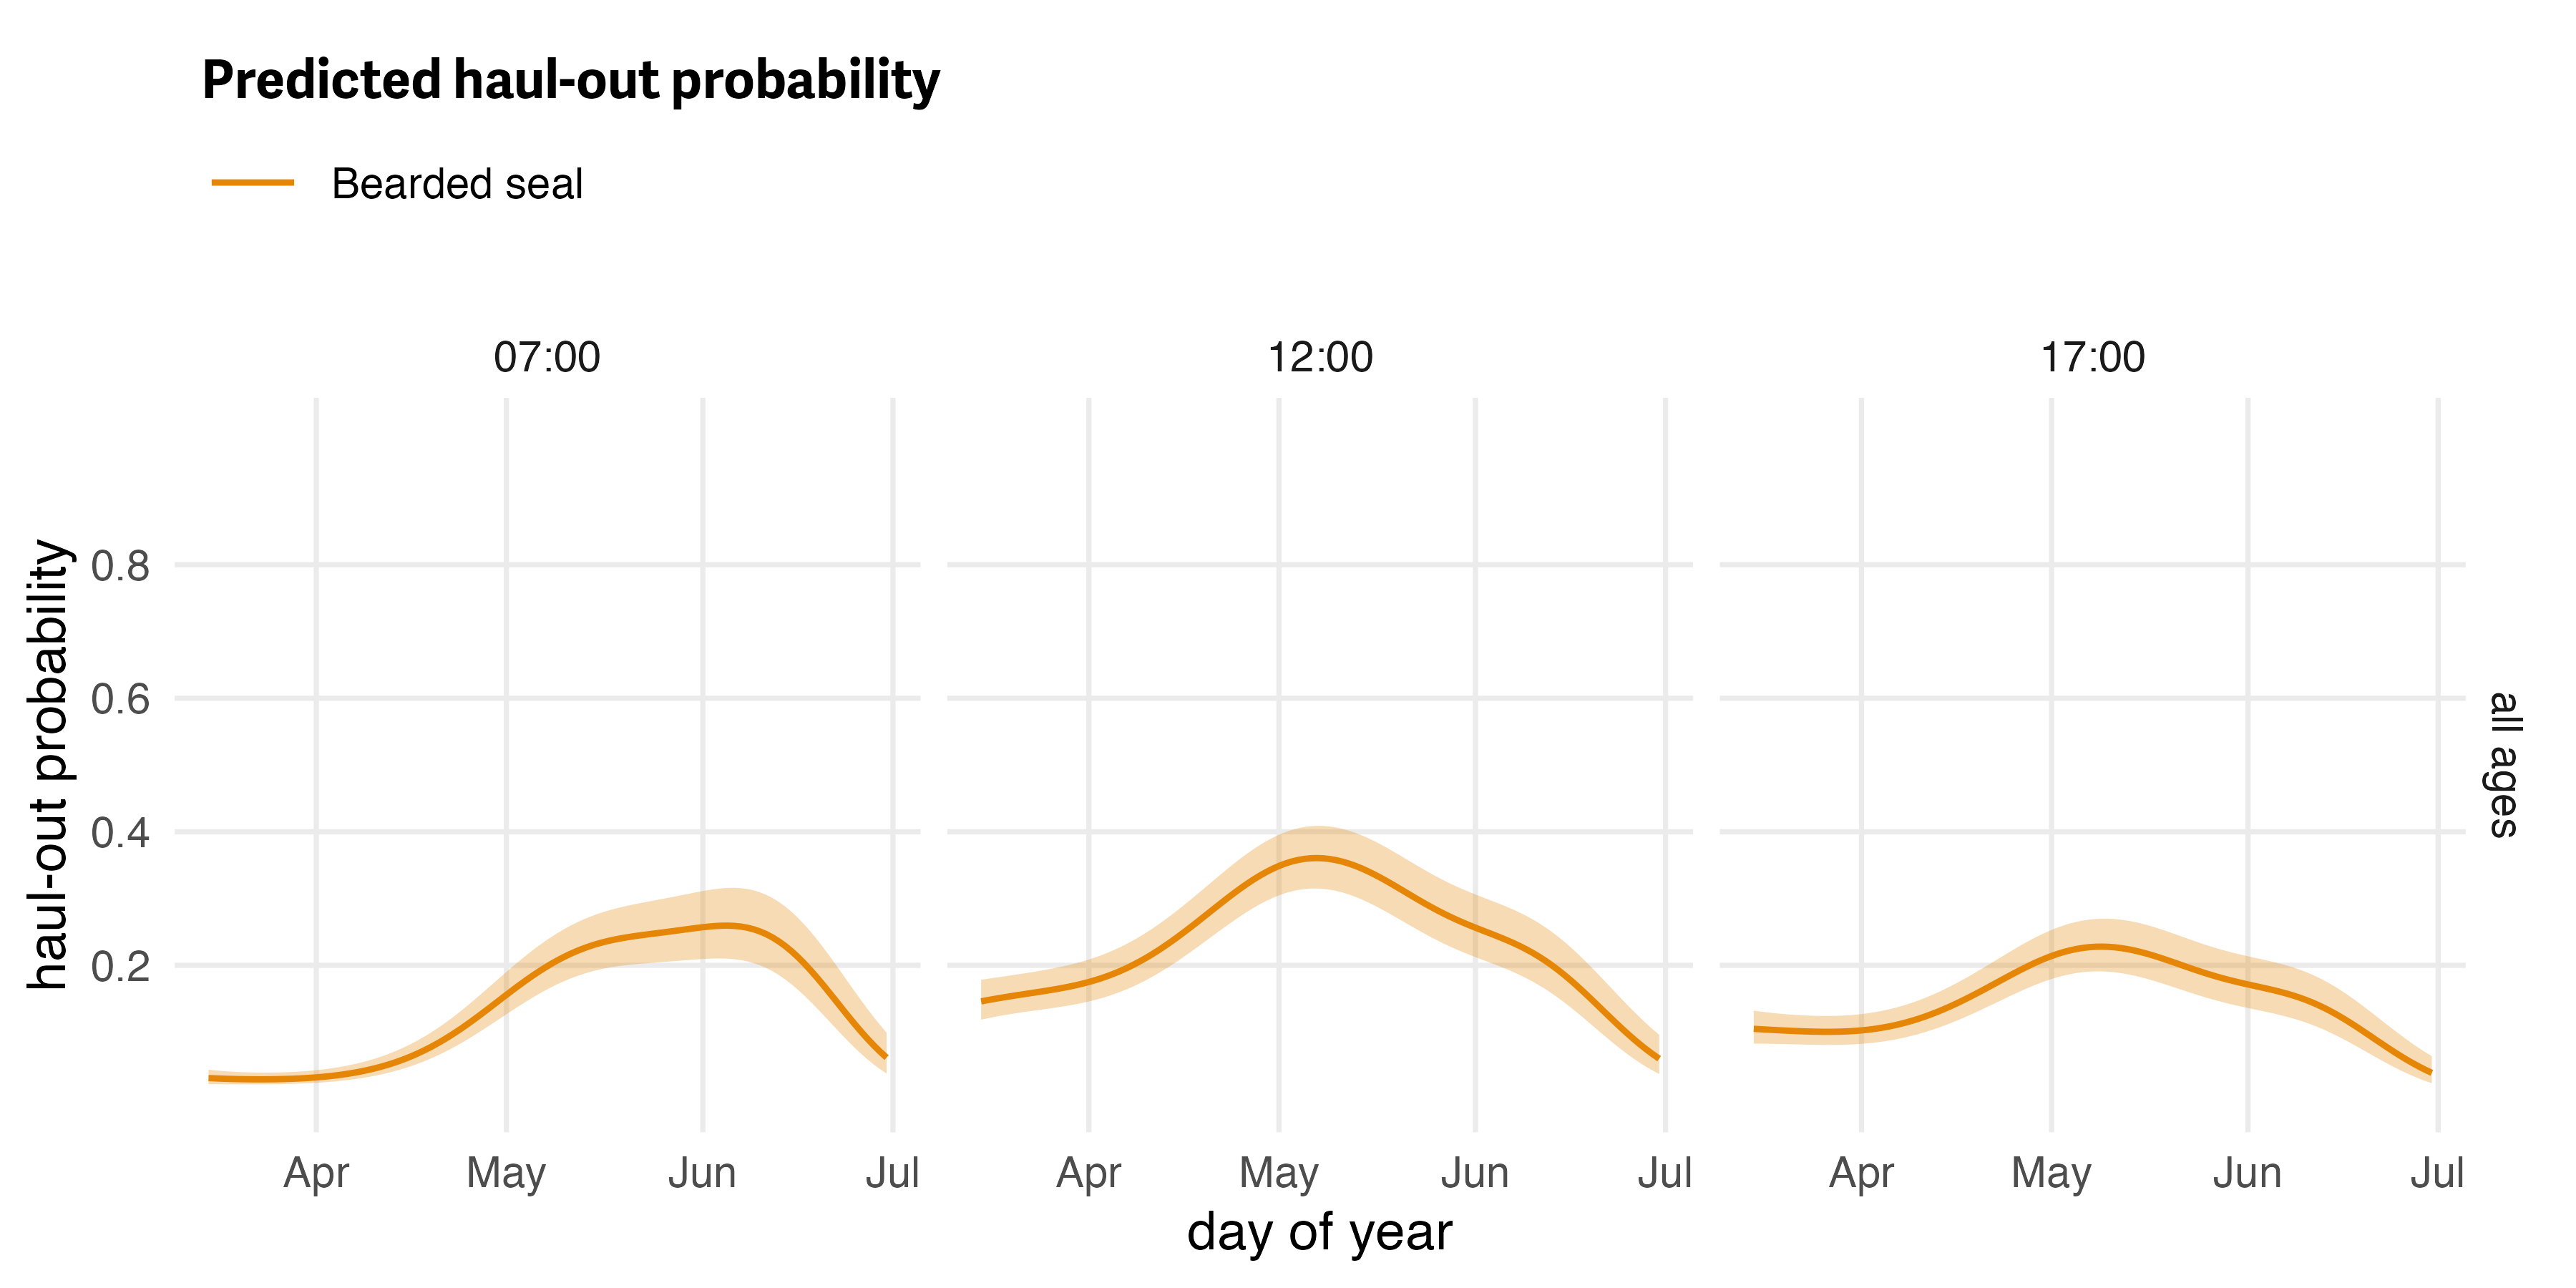
\includegraphics[width=1\linewidth]{../figures/Figure-013} \caption{\textbf{Seasonal variability in haul-out probability and the associated 95\% confidence intervals (shaded area) for bearded seals.} \linebreak Model predictions are shown for three local solar hours (07:00, 12:00, and 17:00). Weather covariate values in the prediction were based on a simple generalized additive model for each weather covariate with smooth terms for day-of-year and solar hour to account for anticipated variability within a day over the season. Age and sex classes are combined into a single `all ages' category.}\label{fig:beardedPredSE}
\end{figure}



\begin{figure}
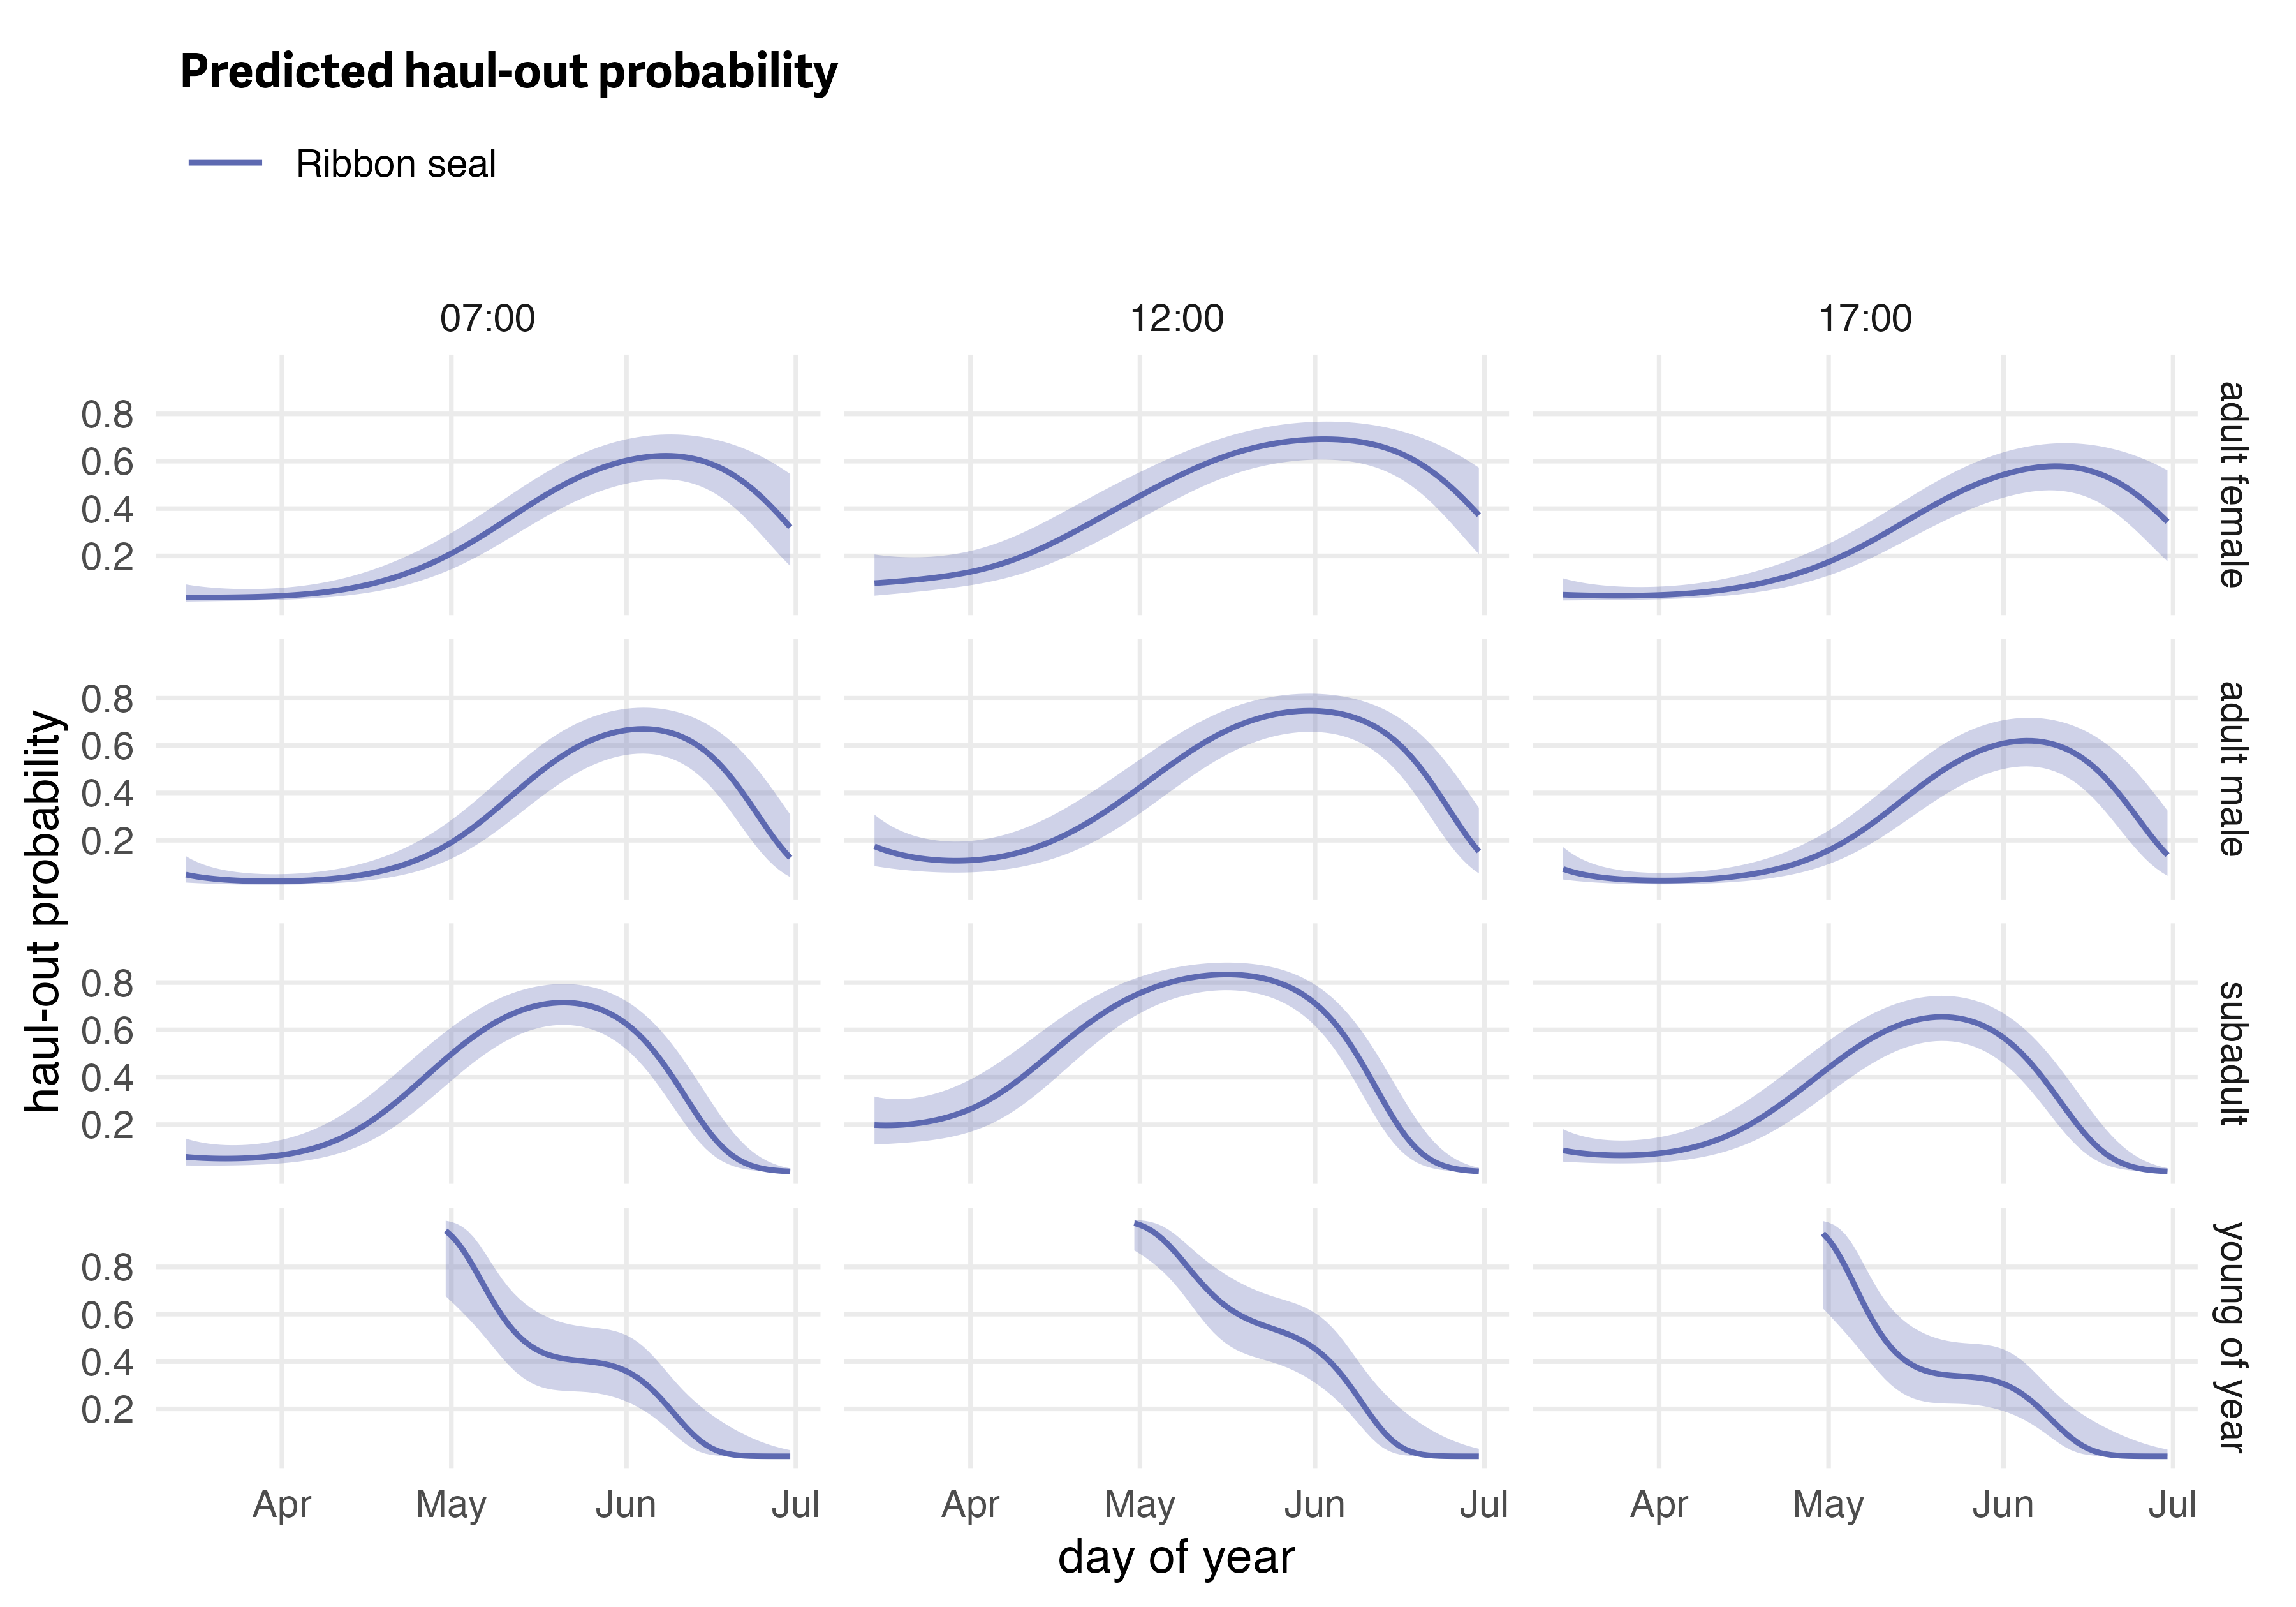
\includegraphics[width=1\linewidth]{../figures/Figure-014} \caption{\textbf{Seasonal variability in haul-out probability and the associated 95\% confidence intervals (shaded area) for ribbon seals.} \linebreak Model predictions are shown for three local solar hours (07:00, 12:00, and 17:00). Weather covariate values in the prediction were based on a simple generalized additive model for each weather covariate with smooth terms for day-of-year and solar hour to account for anticipated variability within a day over the season. Age and sex classes are separated to allow comparisons.}\label{fig:ribbonPredSE}
\end{figure}



\begin{figure}
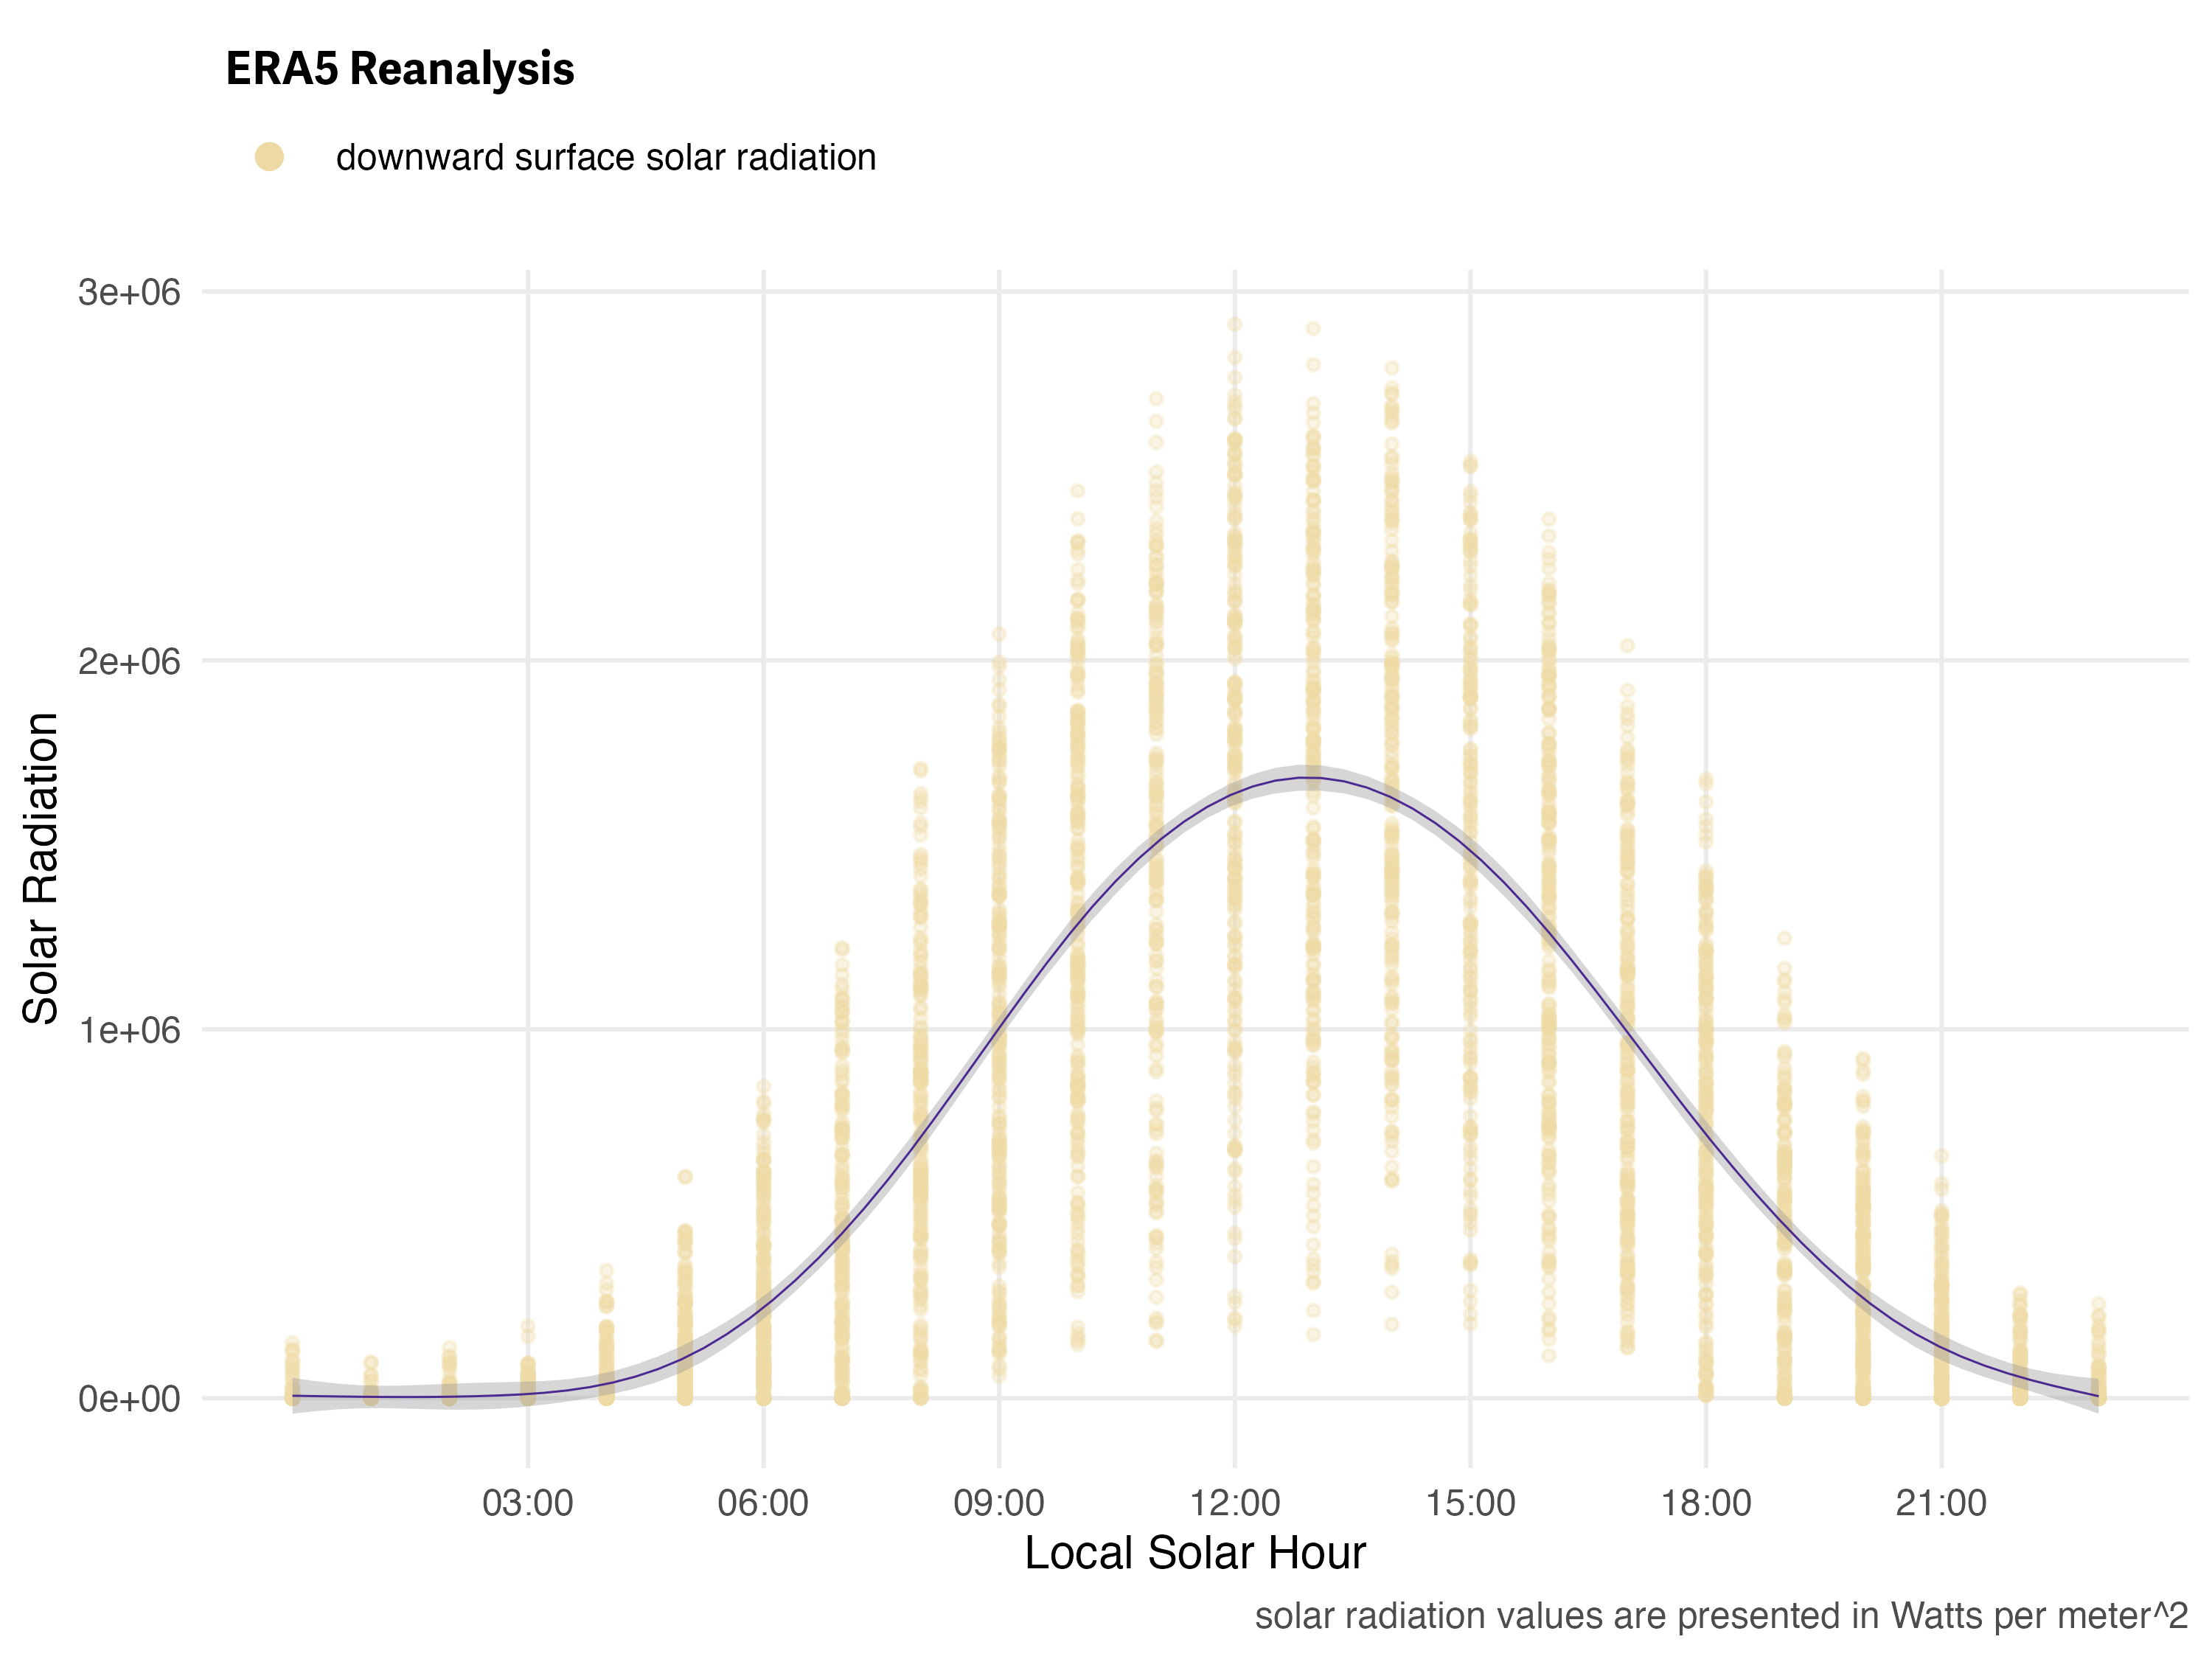
\includegraphics[width=1\linewidth]{../figures/Figure-015} \caption{\textbf{Seasonal variability in haul-out probability and the associated 95\% confidence intervals (shaded area) for spotted seals.} \linebreak Model predictions are shown for three local solar hours (07:00, 12:00, and 17:00). Weather covariate values in the prediction were based on a simple generalized additive model for each weather covariate with smooth terms for day-of-year and solar hour to account for anticipated variability within a day over the season. Age and sex classes are separated to allow comparisons.}\label{fig:spottedPredSE}
\end{figure}

\clearpage

\subsection{Exploring Insolation (Solar Radiation) as a Model Covariate}\label{exploring-insolation-solar-radiation-as-a-model-covariate}

\subsubsection{Introduction}\label{introduction-1}

During the peer review process for this manuscript, Anthony Fischbach suggested
the possibility of using predicted insolation (or solar radiation) values from
the reanalysis model as a more direct and, potentially, more informative
predictor of the daily haul-out cycle in seals compared to time of day. The
notion being that seals are, likely, directly responding to changes in solar radiation
throughout the day and not what time of day it is (i.e.~seals don't have human
watches). Additionally, given the energetic benefits of increased solar
radiation it could be more informative as we would expect seals might have a
higher haul-out probability on sunnier days and for there to be geographic
variability in haul-out behavior associated with geographical differences in
insolation. This approach has an additional benefit of being more parsimonious
compared to our use of the Fourier series or other approaches to represent
hour-of-day in the model (e.g.~24 factors for each hour).

Because of these reasons, we considered and explored this
possibility for our model and the analysis presented in this manuscript. A key
drawback to reliance on solar radiation, in our minds, is that we would lose
insight regarding potential diel patterns -- solar radiation does not
differentiate between dusk or dawn. Bi-modal patterns have been
previously observed in ringed seals and our results in this analysis show some indication of
increased haul-out probability during dawn compared to dusk periods for bearded seals
and some age and sex classes for ribbon and spotted seals.
For other phocid species, increased haul-out probability before solar noon or after
solar noon has been observed. Importantly, understanding these relationships
between haul-out probability and hour-of-day can have important ramifications
on aerial survey study design -- a key focus of this paper.\\
Another hesitation we had was that solar radiation estimates from reanalysis models have
not been previously used as a model covariate within a published study of
pinniped haul-out behavior. Thus, for this analysis, we chose to keep our
original approach and rely on the Fourier series to capture any hour-of-day
effects.

That said, we think the idea of solar radiation as a model covariate in pinniped
haul-out models is intriguing and worth further exploration. The current
availability and increased accessibility to detailed climate reanalysis
products that include solar radiation is exciting and we encourage future, more
detailed exploration of this as a component in pinniped haul-out analysis. To
provide some inspiration, we present some initial efforts and examples for
comparison.

\subsubsection{Methods}\label{methods-1}

In this manuscript, we rely on the NARR reanalysis model as the source for our
weather covariates. However, since our initiation of this analysis, the ERA5
reanalysis model (\url{https://doi.org/10.24381/cds.adbb2d47}) has become one of the
go-to standards for global climate reanalysis and provides an increased temporal
resolution to hourly (compared to the 3-hour resolution of NARR). The global
coverage of ERA5 provides additional flexibility in that the area of interest is
not limited to North America. The ERA5 model provides a number of solar
radiation parameters and it was important to evaluate and understand each of
these estimates in order to select the one that was likely most relevant to
seals. Here, we used the `surface short-wave (solar) radiation downwards'
parameter. This
parameter is described as \emph{``the amount of solar radiation (also known as shortwave radiation)
that reaches a horizontal plane at the surface of the Earth and comprises both
direct and diffuse solar radiation. To a reasonably good approximation, this
parameter is the model equivalent of what would be measured by a pyranometer (an
instrument used for measuring solar radiation) at the surface''}
(\url{https://codes.ecmwf.int/grib/param-db/?id=169}). Thus, this is the
value which most closely represents the amount of solar radiation likely
felt by a seal hauled out of the water.

ERA5 data is available via the Copernicus climate data store API which can be
queried with the CDS-API Python package
(\url{https://cds.climate.copernicus.eu/api-how-to}). The R code provided here
documents the download of the \emph{surface\_solar\_radiation\_downwards} parameter for
our study area of interest and years of interest. The \texttt{reticulate} R package
(\url{https://CRAN.R-project.org/package=reticulate}) allowed interaction with Python.
Additionally, note, extra steps are required to download data on either side
of the 180 anti-meridian.

\begin{Shaded}
\begin{Highlighting}[]
\FunctionTok{library}\NormalTok{(tidyverse)}
\FunctionTok{library}\NormalTok{(reticulate)}
\FunctionTok{library}\NormalTok{(sf)}
\FunctionTok{library}\NormalTok{(terra)}

\CommentTok{\#import python CDS{-}API}
\NormalTok{cdsapi }\OtherTok{\textless{}{-}} \FunctionTok{import}\NormalTok{(}\StringTok{\textquotesingle{}cdsapi\textquotesingle{}}\NormalTok{)}
\CommentTok{\#for this step there must exist the file .cdsapirc}
\NormalTok{server }\OtherTok{=}\NormalTok{ cdsapi}\SpecialCharTok{$}\FunctionTok{Client}\NormalTok{() }\CommentTok{\#start the connection}

\NormalTok{get\_era5 }\OtherTok{\textless{}{-}} \ControlFlowTok{function}\NormalTok{(y) \{}
  \CommentTok{\#we create the query}
\NormalTok{  query }\OtherTok{\textless{}{-}} \FunctionTok{r\_to\_py}\NormalTok{(}
    \FunctionTok{list}\NormalTok{(}
      \AttributeTok{variable =} \StringTok{"surface\_solar\_radiation\_downwards"}\NormalTok{,}
      \AttributeTok{product\_type =} \StringTok{"reanalysis"}\NormalTok{,}
      \AttributeTok{area =} \StringTok{"75/152/47/180"}\NormalTok{, }\CommentTok{\# North, West, South, East}
      \AttributeTok{year =}\NormalTok{ y,}
      \AttributeTok{month =} \FunctionTok{str\_pad}\NormalTok{(}\DecValTok{2}\SpecialCharTok{:}\DecValTok{7}\NormalTok{, }\DecValTok{2}\NormalTok{, }\StringTok{"left"}\NormalTok{, }\StringTok{"0"}\NormalTok{),}
      \AttributeTok{day =} \FunctionTok{str\_pad}\NormalTok{(}\DecValTok{1}\SpecialCharTok{:}\DecValTok{31}\NormalTok{, }\DecValTok{2}\NormalTok{, }\StringTok{"left"}\NormalTok{, }\StringTok{"0"}\NormalTok{),}
      \AttributeTok{time =} \FunctionTok{str\_c}\NormalTok{(}\DecValTok{0}\SpecialCharTok{:}\DecValTok{23}\NormalTok{, }\StringTok{"00"}\NormalTok{, }\AttributeTok{sep =} \StringTok{":"}\NormalTok{) }\SpecialCharTok{\%\textgreater{}\%} \FunctionTok{str\_pad}\NormalTok{(}\DecValTok{5}\NormalTok{, }\StringTok{"left"}\NormalTok{, }\StringTok{"0"}\NormalTok{),}
      \AttributeTok{format =} \StringTok{"netcdf"}
\NormalTok{    )}
\NormalTok{  )}
  \CommentTok{\#query to get the ncdf}
\NormalTok{  server}\SpecialCharTok{$}\FunctionTok{retrieve}\NormalTok{(}\StringTok{"reanalysis{-}era5{-}single{-}levels"}\NormalTok{,}
\NormalTok{                  query,}
                  \FunctionTok{paste0}\NormalTok{(}\StringTok{"era5\_ssrd\_"}\NormalTok{, y, }\StringTok{"\_left.nc"}\NormalTok{))}
  
\NormalTok{  query }\OtherTok{\textless{}{-}} \FunctionTok{r\_to\_py}\NormalTok{(}
    \FunctionTok{list}\NormalTok{(}
      \AttributeTok{variable =} \StringTok{"surface\_solar\_radiation\_downwards"}\NormalTok{,}
      \AttributeTok{product\_type =} \StringTok{"reanalysis"}\NormalTok{,}
      \AttributeTok{area =} \StringTok{"75/{-}180/47/{-}142"}\NormalTok{, }\CommentTok{\# North, West, South, East}
      \AttributeTok{year =}\NormalTok{ y,}
      \AttributeTok{month =} \FunctionTok{str\_pad}\NormalTok{(}\DecValTok{2}\SpecialCharTok{:}\DecValTok{7}\NormalTok{, }\DecValTok{2}\NormalTok{, }\StringTok{"left"}\NormalTok{, }\StringTok{"0"}\NormalTok{),}
      \AttributeTok{day =} \FunctionTok{str\_pad}\NormalTok{(}\DecValTok{1}\SpecialCharTok{:}\DecValTok{31}\NormalTok{, }\DecValTok{2}\NormalTok{, }\StringTok{"left"}\NormalTok{, }\StringTok{"0"}\NormalTok{),}
      \AttributeTok{time =} \FunctionTok{str\_c}\NormalTok{(}\DecValTok{0}\SpecialCharTok{:}\DecValTok{23}\NormalTok{, }\StringTok{"00"}\NormalTok{, }\AttributeTok{sep =} \StringTok{":"}\NormalTok{) }\SpecialCharTok{\%\textgreater{}\%} \FunctionTok{str\_pad}\NormalTok{(}\DecValTok{5}\NormalTok{, }\StringTok{"left"}\NormalTok{, }\StringTok{"0"}\NormalTok{),}
      \AttributeTok{format =} \StringTok{"netcdf"}
\NormalTok{    )}
\NormalTok{  )}
  \CommentTok{\#query to get the ncdf}
\NormalTok{  server}\SpecialCharTok{$}\FunctionTok{retrieve}\NormalTok{(}\StringTok{"reanalysis{-}era5{-}single{-}levels"}\NormalTok{,}
\NormalTok{                  query,}
                  \FunctionTok{paste0}\NormalTok{(}\StringTok{"era5\_ssrd\_"}\NormalTok{, y, }\StringTok{"\_right.nc"}\NormalTok{))}

\NormalTok{\}}

\NormalTok{years }\OtherTok{\textless{}{-}} \FunctionTok{as.character}\NormalTok{(}\DecValTok{2005}\SpecialCharTok{:}\DecValTok{2021}\NormalTok{)}
\ControlFlowTok{for}\NormalTok{(i }\ControlFlowTok{in} \DecValTok{1}\SpecialCharTok{:}\FunctionTok{length}\NormalTok{(years)) \{}
  \FunctionTok{get\_era5}\NormalTok{(years[i])}
\NormalTok{\}}
\end{Highlighting}
\end{Shaded}

To explore performance of our solar radiation parameter within a haul-out model
we replaced the various Fourier series parameters in our model from the manuscript
with the ERA5 \emph{surface solar radiation downwards} (\texttt{era\_ssrd\_watts}) parameter. As
with other reanalysis values (from NARR) in the manuscript, the \texttt{era-ssrd-watts}
values are matched in time and space to the seal haul-out observation data; we
use the full hourly temporal resolution from ERA5. The glmmLDTS framework used
in the paper does not allow for model comparisons with AIC because of
the reliance on pseudo-likelihood. The \texttt{bam()} function within the \texttt{mgcv} package
provides a quick model fitting option that also allowed us to do some model
comparison with AIC. This approach was sufficient for the general demonstration and
exploration purposes here
but future research should consider a range of model fitting frameworks and
approaches that might be more appropriate.

The model specification below was used to specify an \texttt{mgcv::bam()} model that
matched the formula used in the manuscript for ribbon seals. The \texttt{s(speno,\ bs\ =\ "re")}
term is the smooth term for the random effect. All other predictors were
the same.

\begin{Shaded}
\begin{Highlighting}[]
\NormalTok{m1\_ribbon }\OtherTok{\textless{}{-}}\NormalTok{ mgcv}\SpecialCharTok{::}\FunctionTok{bam}\NormalTok{(}
\NormalTok{  dry }\SpecialCharTok{\textasciitilde{}}\NormalTok{ age\_sex }\SpecialCharTok{+} \FunctionTok{s}\NormalTok{(speno, }\AttributeTok{bs =} \StringTok{"re"}\NormalTok{) }\SpecialCharTok{+} 
\NormalTok{    sin1 }\SpecialCharTok{+}\NormalTok{ cos1 }\SpecialCharTok{+}\NormalTok{ sin2 }\SpecialCharTok{+}\NormalTok{ cos2 }\SpecialCharTok{+}\NormalTok{ sin3 }\SpecialCharTok{+}\NormalTok{ cos3 }\SpecialCharTok{+} 
    \FunctionTok{poly}\NormalTok{(day, }\DecValTok{3}\NormalTok{, }\AttributeTok{raw=}\ConstantTok{TRUE}\NormalTok{) }\SpecialCharTok{+} 
\NormalTok{    sin1}\SpecialCharTok{:}\FunctionTok{poly}\NormalTok{(day, }\DecValTok{3}\NormalTok{, }\AttributeTok{raw=}\ConstantTok{TRUE}\NormalTok{) }\SpecialCharTok{+}
\NormalTok{    cos1}\SpecialCharTok{:}\FunctionTok{poly}\NormalTok{(day, }\DecValTok{3}\NormalTok{, }\AttributeTok{raw=}\ConstantTok{TRUE}\NormalTok{) }\SpecialCharTok{+}
\NormalTok{    sin2}\SpecialCharTok{:}\FunctionTok{poly}\NormalTok{(day, }\DecValTok{3}\NormalTok{, }\AttributeTok{raw=}\ConstantTok{TRUE}\NormalTok{) }\SpecialCharTok{+}
\NormalTok{    cos2}\SpecialCharTok{:}\FunctionTok{poly}\NormalTok{(day, }\DecValTok{3}\NormalTok{, }\AttributeTok{raw=}\ConstantTok{TRUE}\NormalTok{) }\SpecialCharTok{+}
\NormalTok{    sin3}\SpecialCharTok{:}\FunctionTok{poly}\NormalTok{(day, }\DecValTok{3}\NormalTok{, }\AttributeTok{raw=}\ConstantTok{TRUE}\NormalTok{) }\SpecialCharTok{+}
\NormalTok{    cos3}\SpecialCharTok{:}\FunctionTok{poly}\NormalTok{(day, }\DecValTok{3}\NormalTok{, }\AttributeTok{raw=}\ConstantTok{TRUE}\NormalTok{) }\SpecialCharTok{+}
\NormalTok{    wind}\SpecialCharTok{*}\NormalTok{temp2m }\SpecialCharTok{+}\NormalTok{ pressure }\SpecialCharTok{+}\NormalTok{ precip }\SpecialCharTok{+} 
\NormalTok{    age\_sex}\SpecialCharTok{:}\FunctionTok{poly}\NormalTok{(day, }\DecValTok{4}\NormalTok{, }\AttributeTok{raw=}\ConstantTok{TRUE}\NormalTok{),}
  \AttributeTok{data =}\NormalTok{ ribbon\_model\_data,}
  \AttributeTok{family =}\NormalTok{ binomial,}
  \AttributeTok{discrete =} \ConstantTok{TRUE}\NormalTok{)}
\end{Highlighting}
\end{Shaded}

Note, the specification for \emph{m1\_ribbon} here does not include
any AR1 structure for temporal autocorrelation. To include this, we needed to
provide a value for \(\rho\) (or \emph{rho}). We examined the autocorrelation within
the model and used the lag-1 value for \(\rho\) .The value for lag-1
autocorrelation was 0.8082 which is
rather high but not surprising. We then updated our model specification with
a value for \(\rho\) as well as the \texttt{A1.start} argument which specifies (as either
\textbf{TRUE} or \textbf{FALSE}) the start point of each block.

\begin{Shaded}
\begin{Highlighting}[]
\NormalTok{m2\_ribbon }\OtherTok{\textless{}{-}}\NormalTok{ mgcv}\SpecialCharTok{::}\FunctionTok{bam}\NormalTok{(}
\NormalTok{  dry }\SpecialCharTok{\textasciitilde{}}\NormalTok{ age\_sex }\SpecialCharTok{+} \FunctionTok{s}\NormalTok{(speno, }\AttributeTok{bs =} \StringTok{"re"}\NormalTok{) }\SpecialCharTok{+} 
\NormalTok{    sin1 }\SpecialCharTok{+}\NormalTok{ cos1 }\SpecialCharTok{+}\NormalTok{ sin2 }\SpecialCharTok{+}\NormalTok{ cos2 }\SpecialCharTok{+}\NormalTok{ sin3 }\SpecialCharTok{+}\NormalTok{ cos3 }\SpecialCharTok{+} 
    \FunctionTok{poly}\NormalTok{(day, }\DecValTok{3}\NormalTok{, }\AttributeTok{raw=}\ConstantTok{TRUE}\NormalTok{) }\SpecialCharTok{+} 
\NormalTok{    sin1}\SpecialCharTok{:}\FunctionTok{poly}\NormalTok{(day, }\DecValTok{3}\NormalTok{, }\AttributeTok{raw=}\ConstantTok{TRUE}\NormalTok{) }\SpecialCharTok{+}
\NormalTok{    cos1}\SpecialCharTok{:}\FunctionTok{poly}\NormalTok{(day, }\DecValTok{3}\NormalTok{, }\AttributeTok{raw=}\ConstantTok{TRUE}\NormalTok{) }\SpecialCharTok{+}
\NormalTok{    sin2}\SpecialCharTok{:}\FunctionTok{poly}\NormalTok{(day, }\DecValTok{3}\NormalTok{, }\AttributeTok{raw=}\ConstantTok{TRUE}\NormalTok{) }\SpecialCharTok{+}
\NormalTok{    cos2}\SpecialCharTok{:}\FunctionTok{poly}\NormalTok{(day, }\DecValTok{3}\NormalTok{, }\AttributeTok{raw=}\ConstantTok{TRUE}\NormalTok{) }\SpecialCharTok{+}
\NormalTok{    sin3}\SpecialCharTok{:}\FunctionTok{poly}\NormalTok{(day, }\DecValTok{3}\NormalTok{, }\AttributeTok{raw=}\ConstantTok{TRUE}\NormalTok{) }\SpecialCharTok{+}
\NormalTok{    cos3}\SpecialCharTok{:}\FunctionTok{poly}\NormalTok{(day, }\DecValTok{3}\NormalTok{, }\AttributeTok{raw=}\ConstantTok{TRUE}\NormalTok{) }\SpecialCharTok{+}
\NormalTok{    wind}\SpecialCharTok{*}\NormalTok{temp2m }\SpecialCharTok{+}\NormalTok{ pressure }\SpecialCharTok{+}\NormalTok{ precip }\SpecialCharTok{+} 
\NormalTok{    age\_sex}\SpecialCharTok{:}\FunctionTok{poly}\NormalTok{(day, }\DecValTok{3}\NormalTok{, }\AttributeTok{raw=}\ConstantTok{TRUE}\NormalTok{),}
  \AttributeTok{data =}\NormalTok{ ribbon\_model\_data,}
  \AttributeTok{family =}\NormalTok{ binomial,}
  \AttributeTok{AR.start =}\NormalTok{ ar1\_start,}
  \AttributeTok{rho =}\NormalTok{ lag1\_ribbon,}
  \AttributeTok{discrete =} \ConstantTok{TRUE}\NormalTok{)}
\end{Highlighting}
\end{Shaded}

The model specification for exploring the use of solar radiation was
specified similarly but without all of the Fourier series parameters and
interactions.

\begin{Shaded}
\begin{Highlighting}[]
\NormalTok{m2\_ssrd\_ribbon }\OtherTok{\textless{}{-}}\NormalTok{ mgcv}\SpecialCharTok{::}\FunctionTok{bam}\NormalTok{(}
\NormalTok{  dry }\SpecialCharTok{\textasciitilde{}}\NormalTok{ age\_sex }\SpecialCharTok{+} \FunctionTok{s}\NormalTok{(speno, }\AttributeTok{bs =} \StringTok{"re"}\NormalTok{) }\SpecialCharTok{+} 
\NormalTok{    era5\_ssrd\_watts }\SpecialCharTok{+}
    \FunctionTok{poly}\NormalTok{(day, }\DecValTok{3}\NormalTok{, }\AttributeTok{raw=}\ConstantTok{TRUE}\NormalTok{) }\SpecialCharTok{+} 
\NormalTok{    era5\_ssrd\_watts}\SpecialCharTok{:}\FunctionTok{poly}\NormalTok{(day, }\DecValTok{3}\NormalTok{, }\AttributeTok{raw=}\ConstantTok{TRUE}\NormalTok{) }\SpecialCharTok{+}
\NormalTok{    wind}\SpecialCharTok{*}\NormalTok{temp2m }\SpecialCharTok{+}\NormalTok{ pressure }\SpecialCharTok{+}\NormalTok{ precip }\SpecialCharTok{+} 
\NormalTok{    age\_sex}\SpecialCharTok{:}\FunctionTok{poly}\NormalTok{(day, }\DecValTok{3}\NormalTok{, }\AttributeTok{raw=}\ConstantTok{TRUE}\NormalTok{),}
  \AttributeTok{data =}\NormalTok{ ribbon\_model\_data,}
  \AttributeTok{family =}\NormalTok{ binomial,}
  \AttributeTok{AR.start =}\NormalTok{ ar1\_start,}
  \AttributeTok{rho =}\NormalTok{ lag1\_ribbon,}
  \AttributeTok{discrete =} \ConstantTok{TRUE}\NormalTok{)}
\end{Highlighting}
\end{Shaded}

The two models were compared with AIC to evaluate whether the
reduction in degrees of freedom with fewer terms in the solar radiation
model was matched with improved explanatory power in the model fit. While the
model and code specified above is for ribbon seals, the same approach was
repeated for bearded and spotted seals.

A similar approach to that presented in this manuscript for prediction was
employed with solar radiation values in lieu of hour of day. For prediction
values, quantiles (5\% increments) of the observed range of ERA5 solar radiation values were
used with 100\% representing the maximum observed solar radiation value. This
allowed similar data visualizations and easier comparisons to those
predictions in the manuscript that include hour of day.

\subsubsection{Results}\label{results-1}

To evaluate whether the solar radiation parameter matched our expectations and
compared well with hour of the day, we visualized the variability of the
\texttt{era5\_ssrd} values within
our study area as they relate to hour of the day (\ref{fig:era5-ssrd-plot}).
The unimodal distribution
is centered around the middle of the solar day with peak solar radiation
coinciding with 13:00 local solar. This suggests solar radiation could be an
informative covariate for capturing unimodal diel patterns in haul-out
behavior.



\begin{figure}
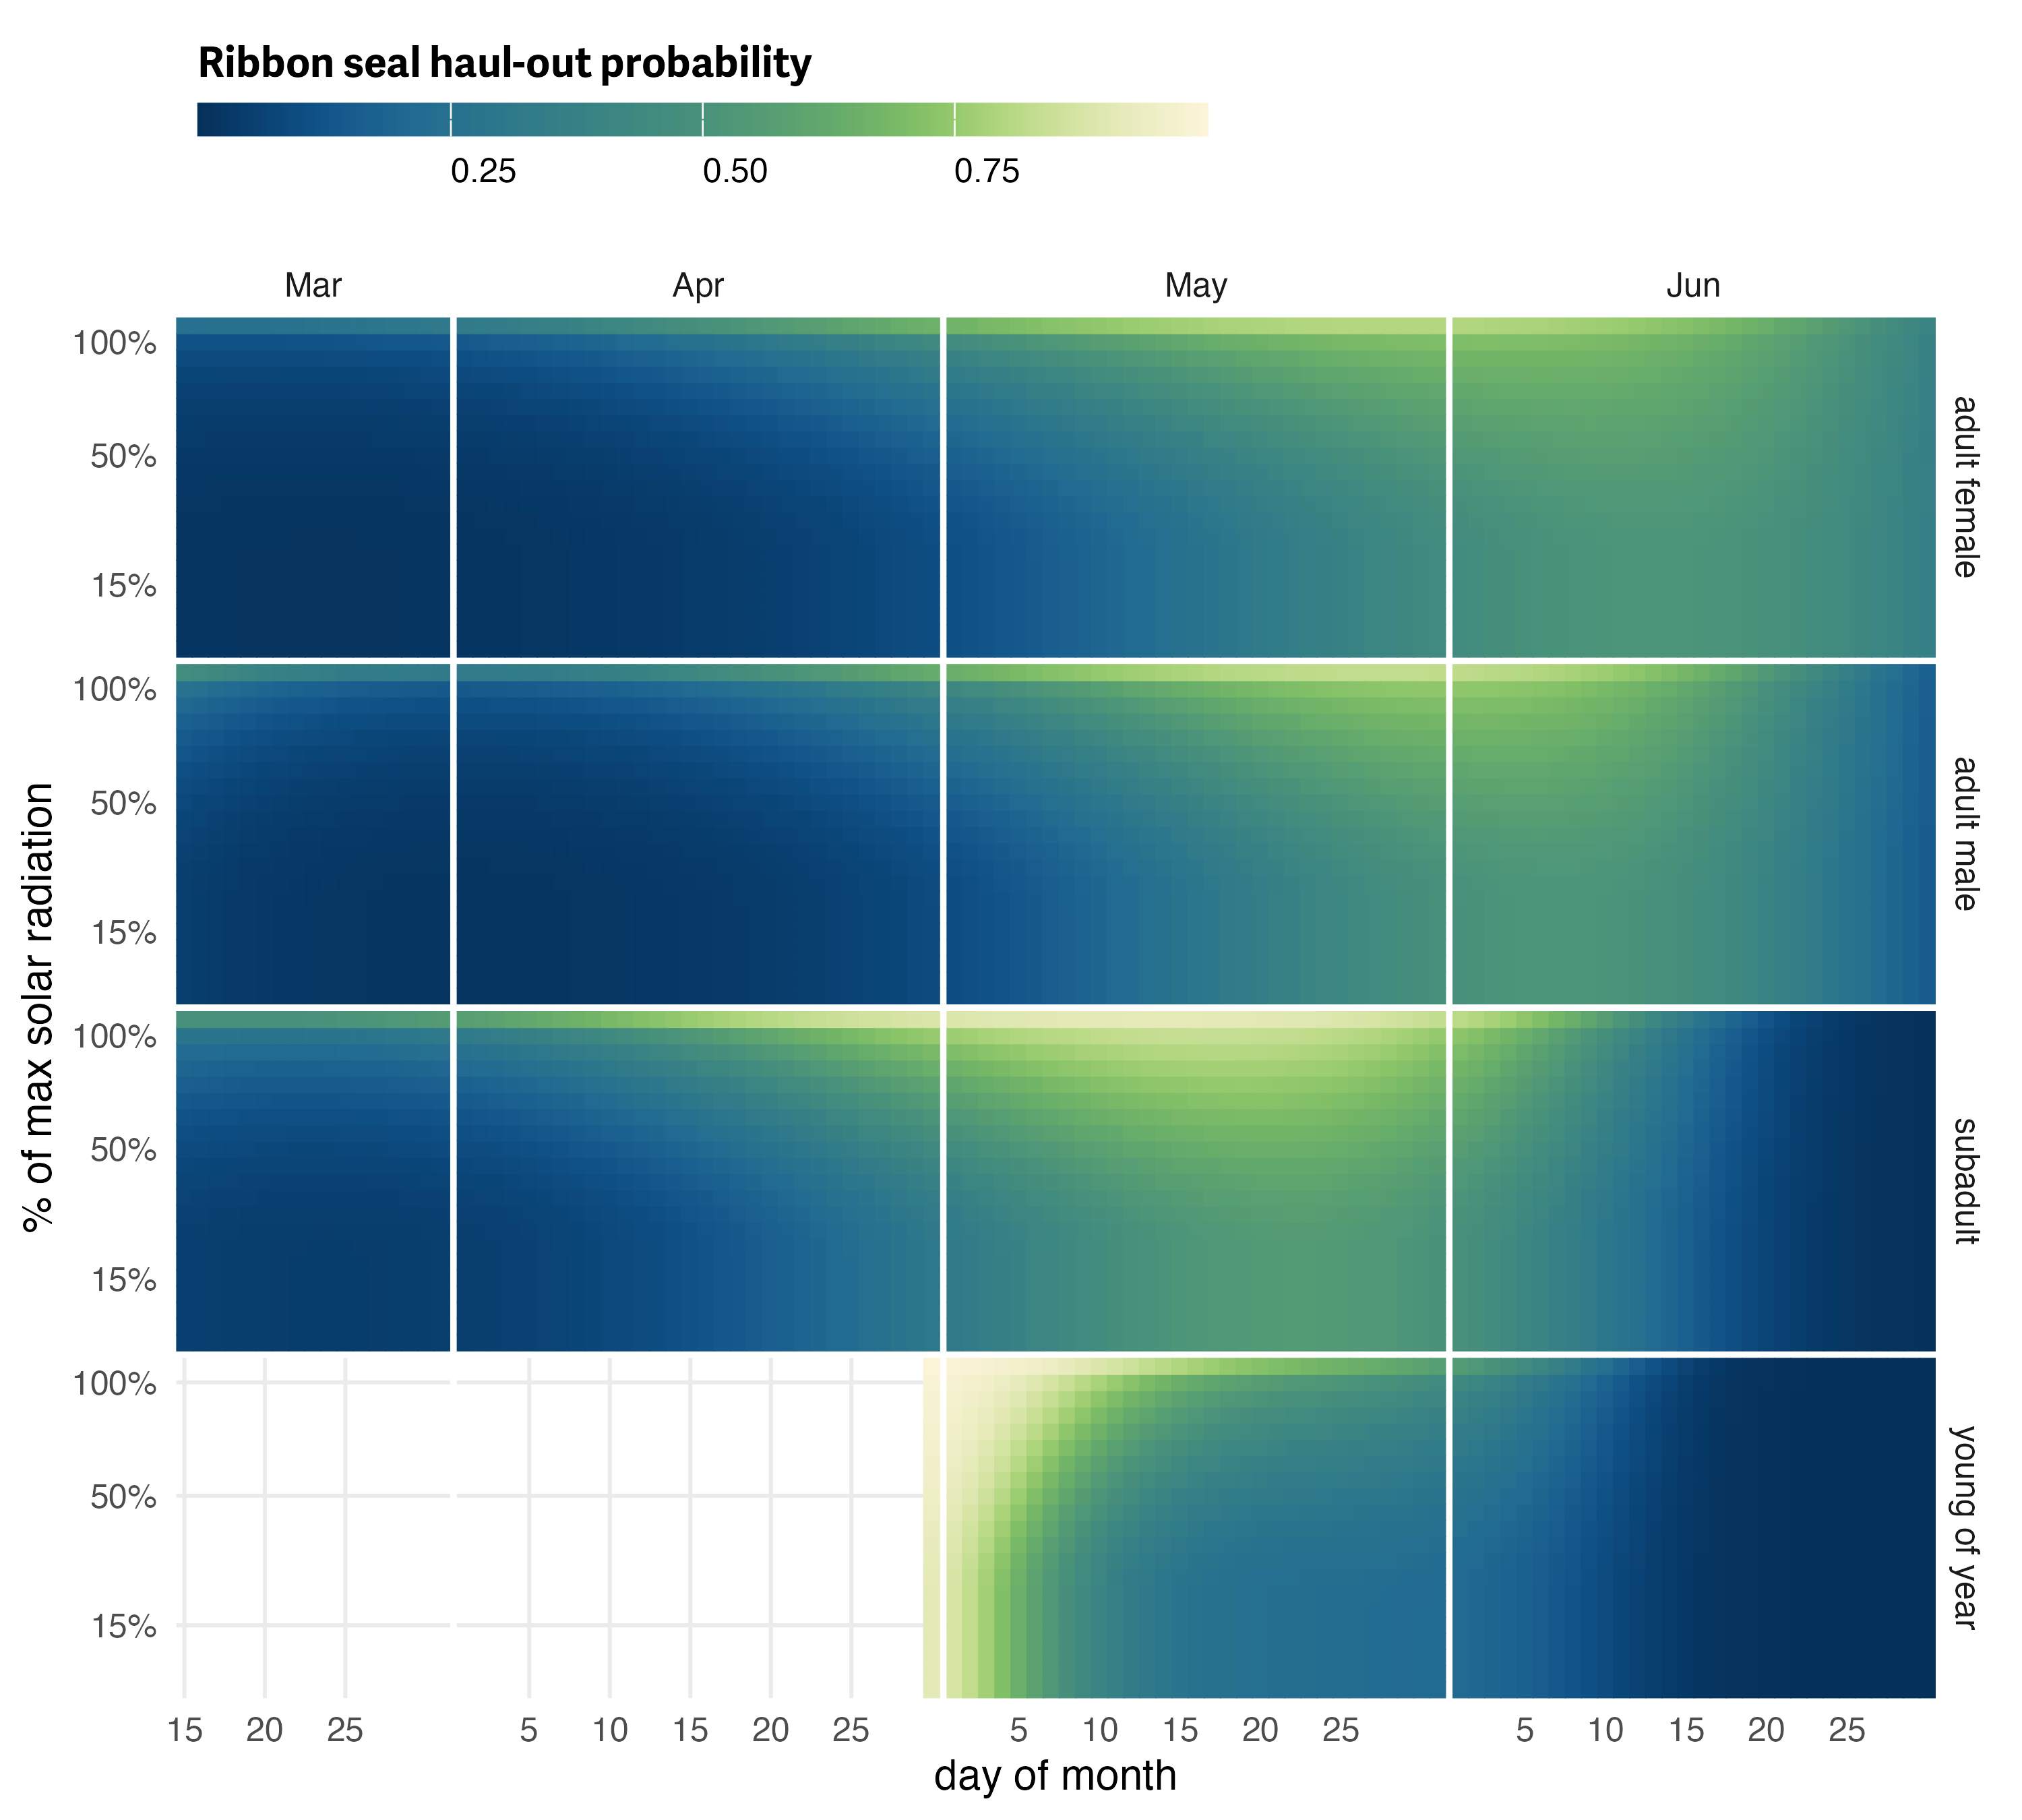
\includegraphics[width=1\linewidth]{../figures/Figure-016} \caption{\textbf{Diel Pattern of Solar Radiation Values from ERA5 Reanalysis.} \linebreak Downward surface solar radiation estimates from the ERA5 climate reanalysis for 5000 random points within the study area between 2005 and 2021. Solar radiation values are presented in Watts per square-meter and the smoothed line highlights the strong diel pattern.}\label{fig:era5-ssrd-plot}
\end{figure}

The bearded seal model matching the specification from the manuscript resulted in
126.13 degrees of freedom and an AIC value of
-7428.929. The model with solar radiation resulted in
39.619 degrees of freedom and an AIC value of
-6797.378. The ribbon seal model matching the specification from the manuscript resulted in
131.478 degrees of freedom and an AIC value of
-16372.29. The model with solar radiation resulted in
115.126 degrees of freedom and an AIC value of
-16038.175. The spotted seal model matching the specification from the manuscript resulted in
125.506 degrees of freedom and an AIC value of
-23584.373. The model with solar radiation resulted in
109.163 degrees of freedom and an AIC value of
-23302.772. Despite the additional terms, the
models with the Fourier series representation of hour of day resulted in a
lower AIC value and were still preferred models for each of the species.

Predictions from the model fits and visualization of those predictions were
produced for each species but, here, we only present visualizations from
ribbon seals as an example (Figure \ref{fig:ssrd-prediction-heatmap} and Figure
\ref{fig:ssrd-ribbonPredSE}). Similar seasonal patterns previously observed were
still apparent with subadults hauling out earlier in the season followed by
adult males and, then, adult females. The observed relationship with hour of
day and the centering of peak haul-out probability around solar noon was
reflected in these predictions as a one-sided distribution with maximum solar
radiation having the highest haul-out probability and minimal solar radiation
the least. The seasonal distribution of haul-out probability along with 95\%
confidence intervals also provided comparable insights (see figures
\ref{fig:ribbonPredSE} and \ref{fig:ssrd-ribbonPredSE}). That said, subtle
differences in the shape and extent of confidence limits were present.



\begin{figure}
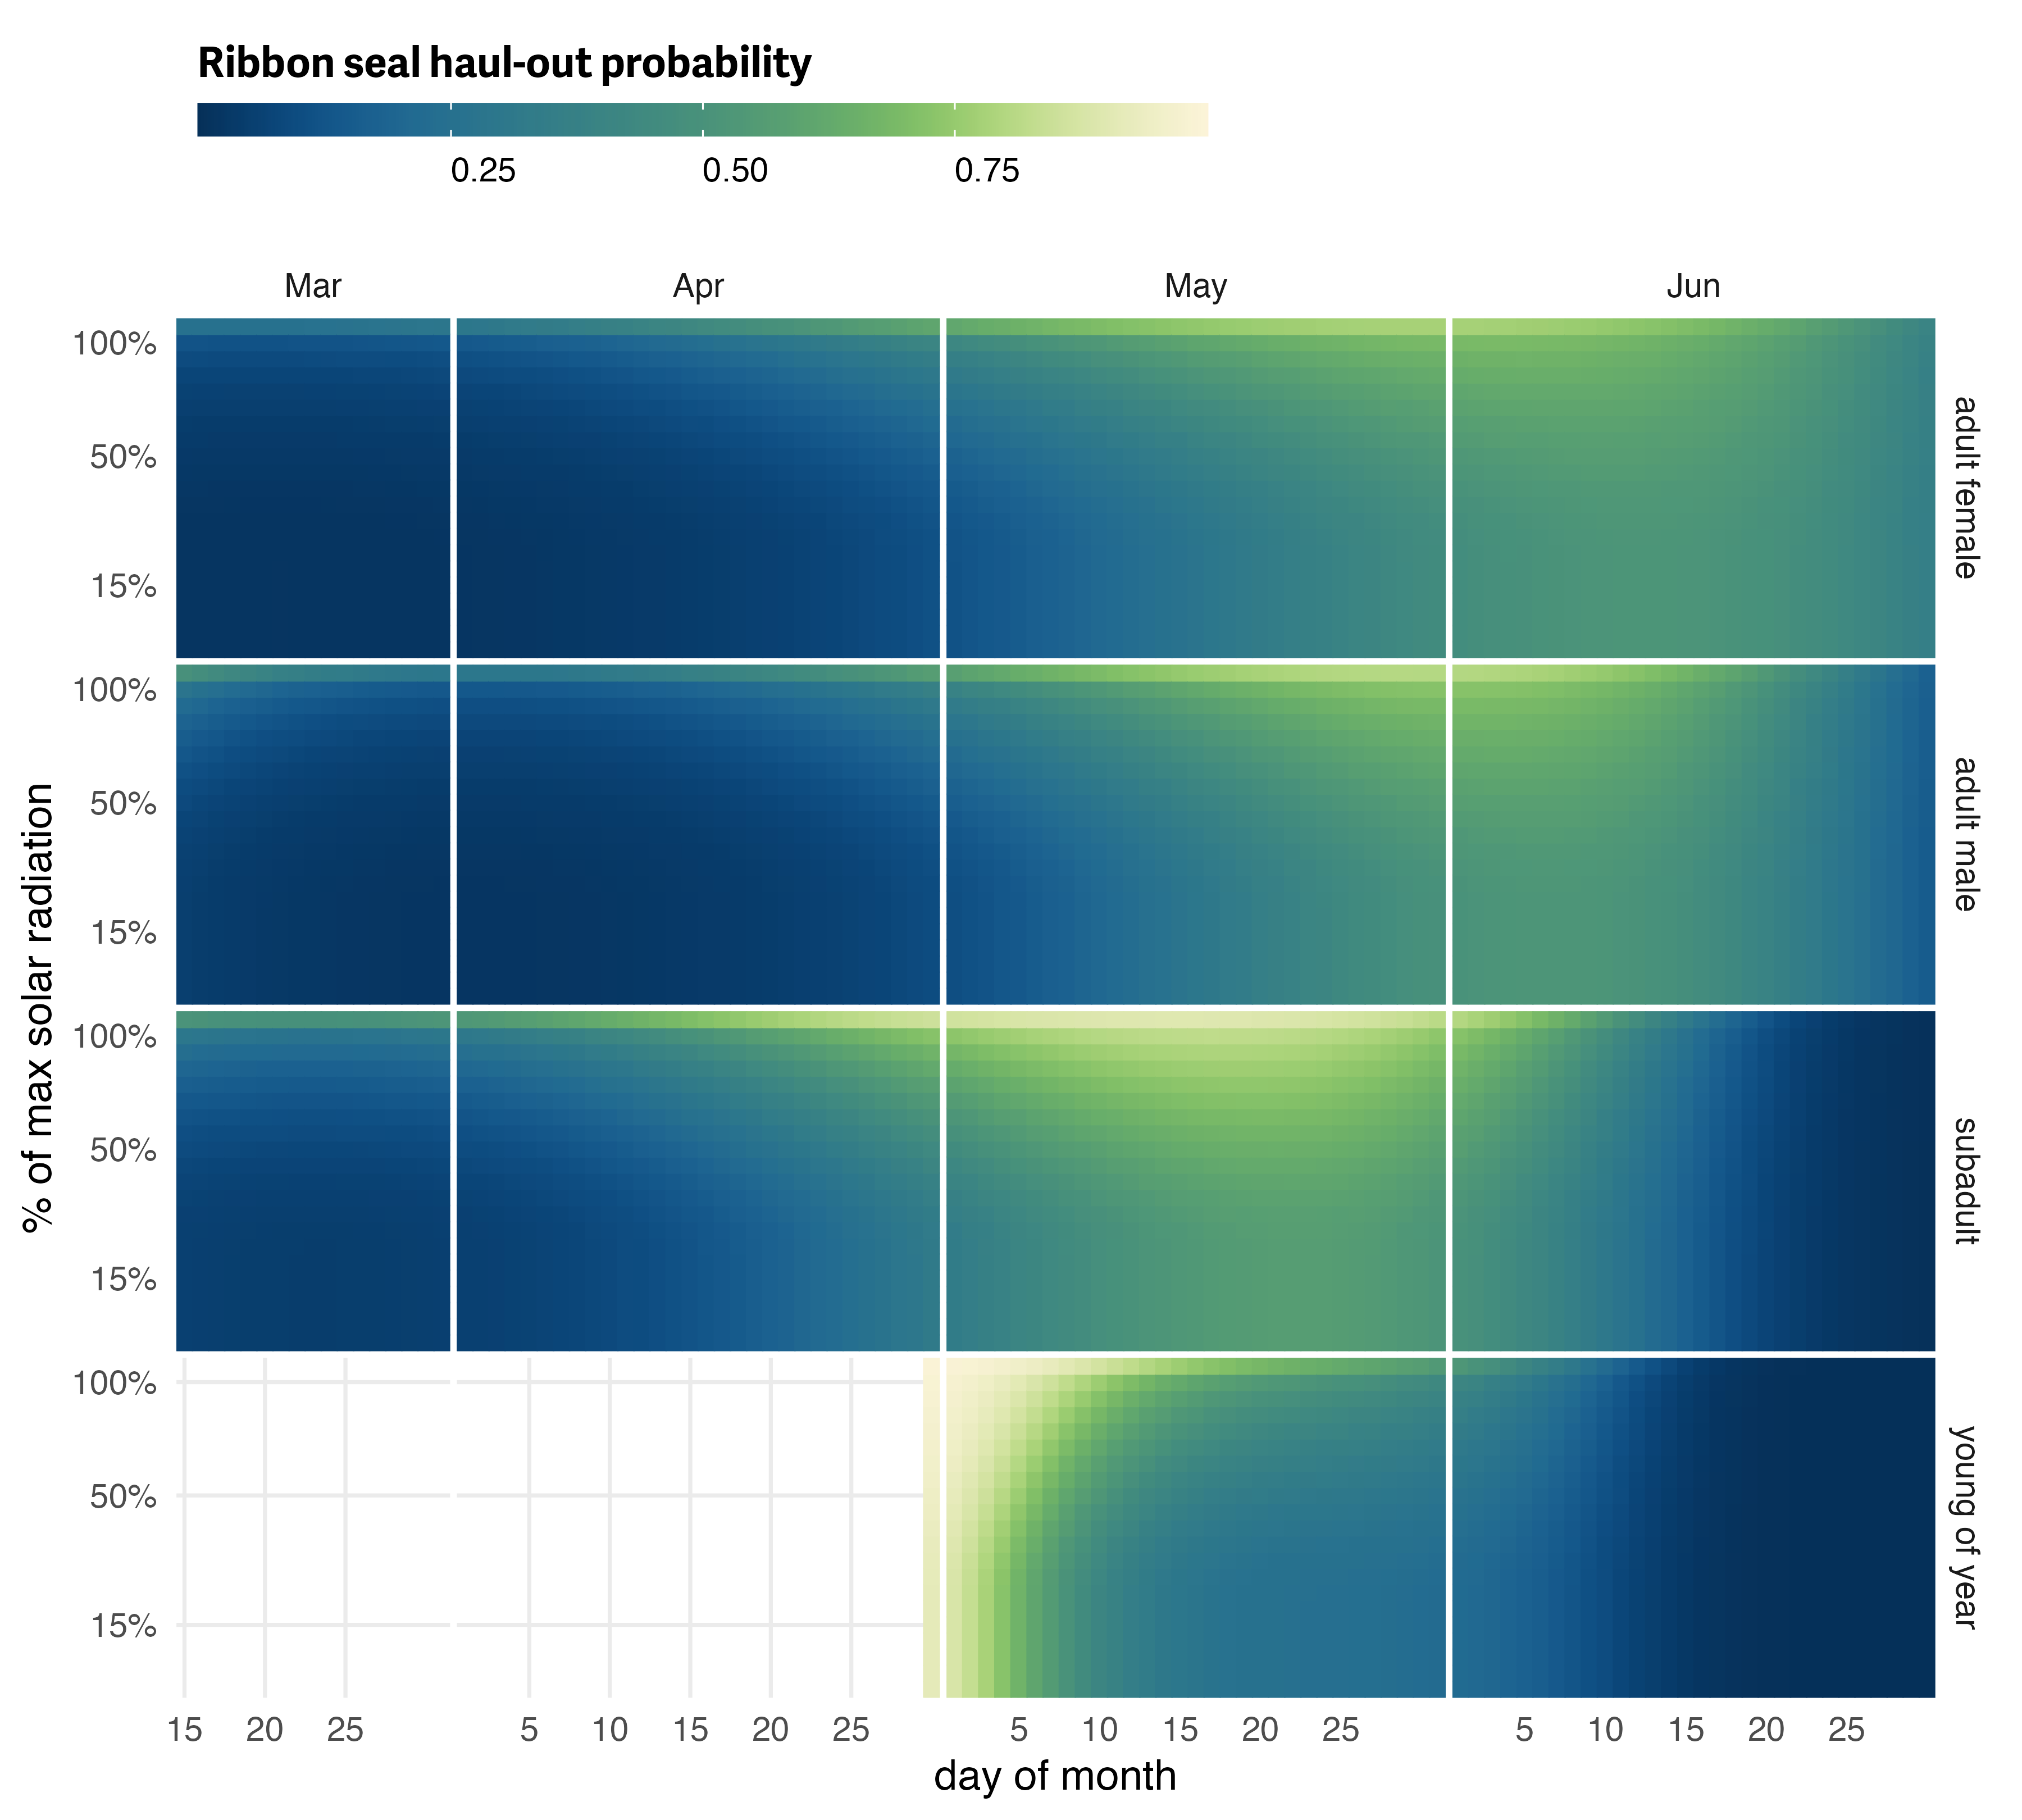
\includegraphics[width=1\linewidth]{../figures/Figure-017} \caption{\textbf{Solar radiation as a predictor of ribbon seal haul-out probability.} \linebreak Predicted haul-out probability of ribbon seals from 15 March to 30 June for each age and sex class used in the model. In this model, solar radiation was used in lieu of hour of day. The apparent seasonal progression with subadults hauling out earlier in the season followed by adult males and, then, adult females is still notable although maybe not as clear. Predictions for young of the year still show their transition from newly weaned pups resting on the ice to more in-water activities. The overall pattern is in agreement with a one-sided view of Figure 7 where maximum solar radiation is equivalent to local solar noon.}\label{fig:ssrd-prediction-heatmap}
\end{figure}



\begin{figure}
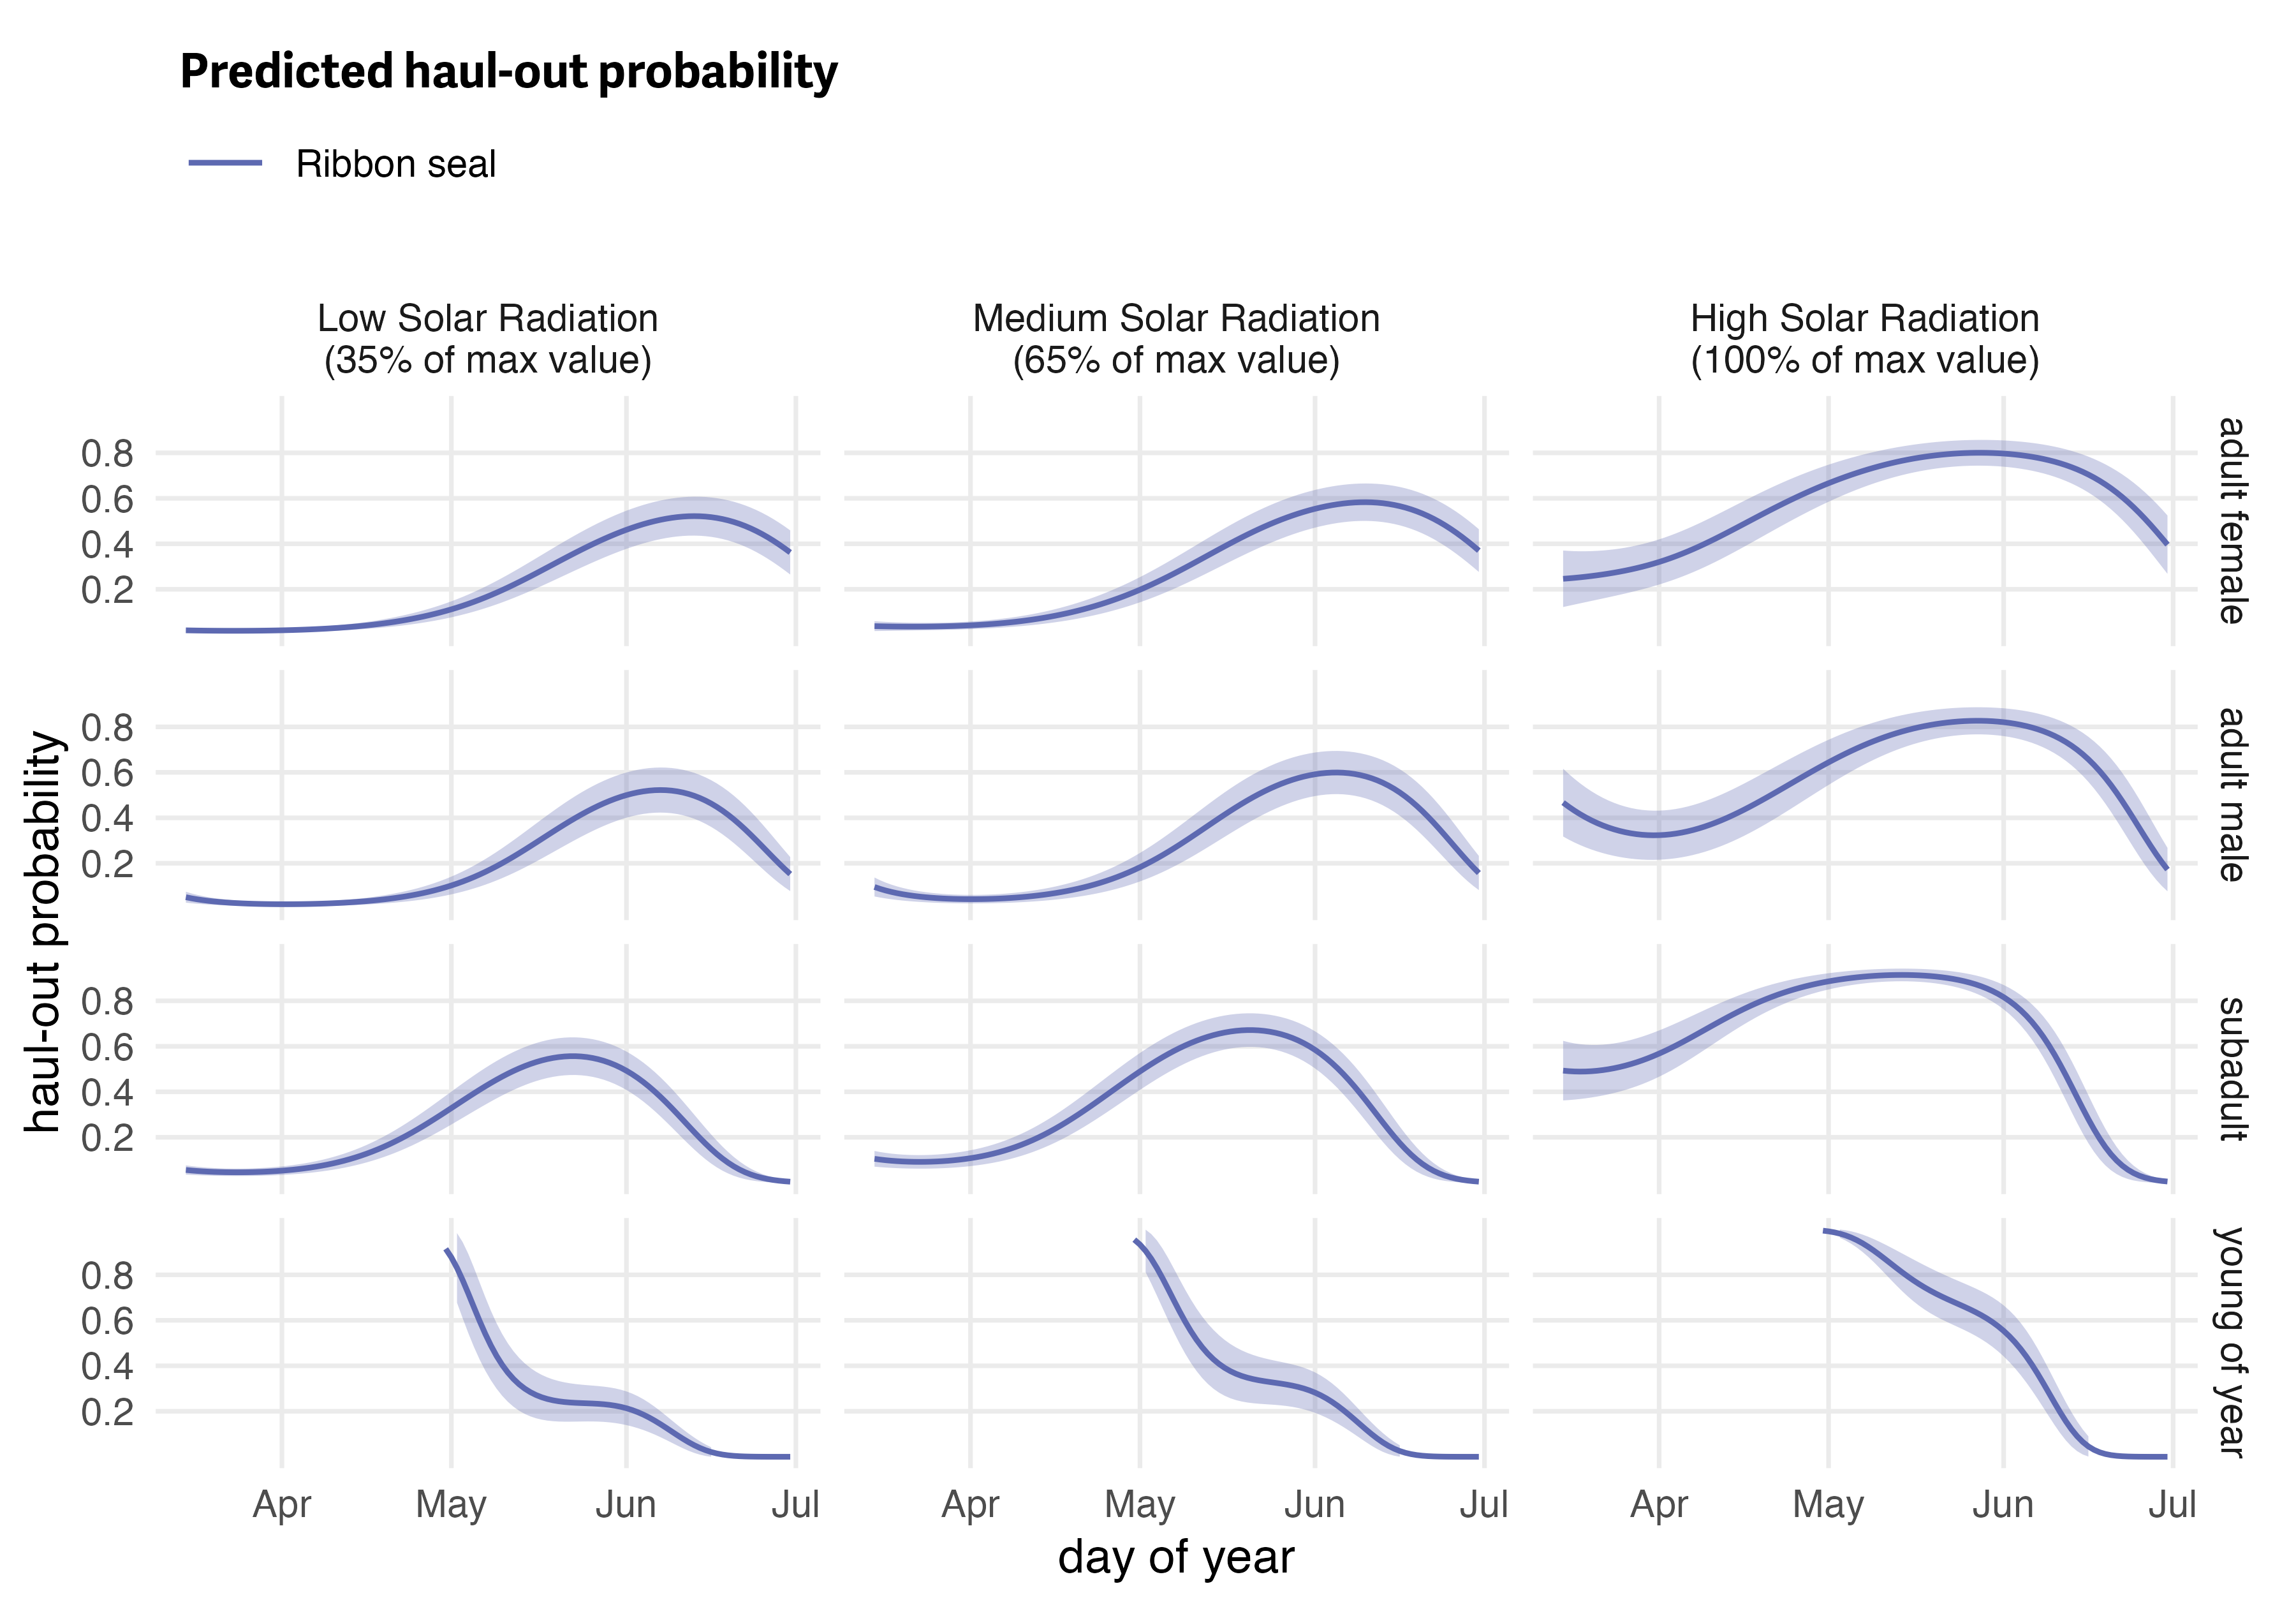
\includegraphics[width=1\linewidth]{../figures/Figure-018} \caption{\textbf{Solar radiation as a predictor of ribbon seal haul-out probability (with uncertainty).} \linebreak Seasonal variability in haul-out probability and the associated 95\% confidence intervals (shaded area) for ribbon seals. In this model predictions are shown for low, medium, and high values of solar radiation (as percentages of the maximum value observed) in lieu of local solar hour. There's general agreement in the overall seasonal patterns between the two approaches but sublte differences in shape and extent of the confidence limits were present (see Figure S2 for comparisons).}\label{fig:ssrd-ribbonPredSE}
\end{figure}

\subsubsection{Discussion}\label{discussion-1}

Solar radiation has potential as an informative covariate in pinniped haul-out
models that can be directly linked to seal physiology and expected behavioral
changes. The ERA5's \emph{surface solar radiation downwards} values aligned with hour
of day and maximum values occurred at or just after local solar noon. This
highlighted the informative potential for this approach. However, despite an
overall reduction in the total number of parameters and degrees of freedom, AIC
comparison still favored the models for each species that included hour of day
as a Fourier series.

This analysis was not intended to be a full comparison --
we simply want to demonstrate the potential and inspire further investigation --
but, there are three possibilities that might explain the preference for hour of
day. First, there are a broad range of solar radiation values represented for each
hour of the day. Cloud cover, fog, and precipitation all reduce downward solar
radiation at the surface and we might expect this to impact haul-out
probability. However, the photoperiod and the timing of sunrise and sunset are
not impacted by weather and seals may be responding to these signals more than
the amount of solar radiation. Additionally, this study spans a range of
physiological cycles and energetic needs and higher solar radiation may not be a
consistent driving influence on seals. Increased energy from the sun may be
important during molt but less so during pupping and breeding periods. Second,
the timing and duration of haul-out behavior may also be influenced by diel
patterns in weather (e.g.~lower winds in the morning) or ecosystem dynamics
(e.g.~prey availability) that lead to a skewness in the distribution of haul-out
behavior that wouldn't be reliably captured by solar radiation values. Third,
this effort is only an initial effort to explore the use of solar radiation in
pinniped haul-out models. A more in depth and rigorous exploration of this topic
might discover an approach that results in a more parsimonious and preferred
model formulation.

Again, we want to acknowledge Anthony Fischbach for the suggestion during the
peer review process. We think this is an excellent example of the peer review
process working to improve the quality of our manuscript and advance the
scientific process. We hope others will take our example and expand on it
within future analyses.



\end{document}
